\chapter{Literature Review}
\label{ch:2}

The aim of the current study is to investigate which phonetic patterns in non-native (L2) English speech are judged to be foreign accented by native (L1) listeners of American English. This chapter provides an overview of research on phonetic and phonological characteristics of foreign accent, after which the focus shifts to relevant theories of speech perception and lexical identification. Based on the findings and theories in previous literature, the rationale for the hypothesis of the current study is further discussed. 

\section{Segmental Correlates of Foreign Accent}

Previous literature often suggests that consonant variations are associated with perceived accentedness (e.g., \citealt{Flege_1994, Magen_1998}). \citet{Major_1987} found that L2 English speakers’ production of English Voice Onset Time (VOT) correlates with perceived accentedness. He found that the closer the L2 VOT conforms to the American English norm (i.e., mean L1 VOT), the higher the accentedness score (i.e., the more native-like a speaker is perceived).  \citet{Gonzalez-Bueno_1997} similarly showed that VOT affects the degree of perceived accentedness. In her study, the Spanish /k/s produced by English speakers with a VOT outside of an L1 Spanish speaker’s range, which is between 15 to 35 milliseconds (ms), were rated as very accented by monolingual Spanish speakers. This suggests that L1 Spanish speakers are also sensitive to the temporal boundaries of plosive consonants. 

L2 liquid consonant variations (e.g., using [r, ɾ] instead of [l, ɹ]) might also be associated with foreign accent. For example, the substitution of the Japanese flap (i.e., [ɾ]) for the English liquids [l] and [ɹ] was found to be indicative of foreign accent by L1 English speakers \citep{Riney_2000}. \citet{Solon_2015} studied English speakers’ L2 pronunciation of the Spanish [l].  When English speakers pronounced a Spanish [l] as a velarized English [lˠ], the sound was rated as very foreign accented by L1 Spanish speakers. \citet{Solon_2015} further showed that the degree of foreign accentedness of the non-Spanish-like [lˠ] depends on the degree of velarization, as measured by the frequency of the second formant (F2) and the duration of the L2 [lˠ]. The lower the F2, the shorter the non-native [lˠ] and the more foreign-accented the L2 [lˠ] sounds to native Spanish speakers. Although previous research did show that consonant variations (e.g., VOT-shortening, [ɹ, l] to [ɾ]) could affect accentedness judgments, the types of consonant variations discussed in previous literature were limited, with most of the research focusing on plosives and liquids. To further validate the effect of consonant variations on foreign accent perception, evidence is needed for whether other types of consonant variations (e.g., feature changes in fricatives) lead to similar accentedness judgments.

\citet{Major_1987} focused on vowel perceptions. He showed that foreign accentedness might be associated with some vowels, but not with others. In his study, L1 American English listeners first provided accentedness ratings of L2 productions of the English word “\textit{bet}” ([bɛt]) and “\textit{sat}” ([sæt]). The initial consonants were then edited out, leaving only the vowels and the codas (i.e., [ɛt] and [æt]). Another group of L1 English listeners were presented with these stimuli (i.e., [ɛt]s and [æt]s) in an identification test. The task was to determine whether the stimulus they heard was [ɛt] or [æt]. Accuracy ratings were calculated based on how often a stimulus was correctly identified (e.g., how often an L2 [ɛt] was identified as [ɛt] rather than [æt]).  

The study showed that the accentedness ratings of [sæt] negatively correlated with the accuracy ratings of its rime (e.g., [æt]).  That is, the more accurately the L2 [æt] was identified by L1 English listeners as [æt], the less accented [sæt] sounded. However, the accentedness of [bɛt] positively correlated with the accuracy of its rime [ɛt], suggesting that [bɛt] was rated as being more accented when its rime [ɛt] was more accurately identified as [ɛt]. \citet{Major_1987} thus concluded that whether the pronunciations of vowels have any impact on perceived accentedness depends on the specific vowel in question. 

Similar findings were reported by \citet{Chan_2016}, who used synthesized English phonemes /a/, /æ/ and /ʌ/ as stimuli. In their study, the frequencies of the first (F1) and second formants (F2) and durations of the three vowels were manipulated. L1 English speakers were recruited to provide accentedness judgments on the synthesized stimuli. The results show that the deviations of F1 and F2 from mean L1 frequency values might increase the perceived accentedness for some vowels but decrease the perceived accentedness for other vowels. For example, as F1 and F2 center frequency values became lower than L1 formant frequency values (i.e., mean center frequencies), /a/ and /æ/ were rated as more accented. Surprisingly, when F1 and F2 values of /ʌ/ became lower than mean center formant frequencies of L1 speakers, /ʌ/ became less accented. In other words, the deviation of vowel formant frequencies may either increase or decrease accentedness depending on the specific vowel in question. 

The reason for this phenomenon was attributed to the overlap of vowel space. As the F1 and F2 of /a/ and /æ/ became lower with respect to L1 formant frequency values, /a/ and /æ/ started to overlap with L1 formant frequencies of /ʌ/ and /a/, respectively. In other words, the lowering of F1 and F2 for /a/ and /æ/ made them sound like other vowels to L1 speakers. However, when F1 and F2 values of /ʌ/ became lower, /ʌ/ actually moved away from L1 formant frequencies of /a/ and /æ/. As a result, the degree of overlapping decreased, which in turn decreased the perceptual accentedness. Contrary to findings in \citet{Chan_2016, Major_1987}, \citet{McCullough_2013} found that greater formant deviation from L1 speaker norms leads to higher degrees of accentedness, no matter which vowel is considered. This finding is consistent with several other studies, which also showed independent effects of both static F1 and dynamic/static F2 values on perceived accentedness \citep{Munro_1993, Wayland_1997}. 

Previous research on L2 vowel perception has shown conflicting findings. It could be the case that the L1 speaker norm, from which vowel deviation is usually measured, is not a representative indicator \citep{Chan_2016}. Perhaps vowel perception depends on the spectral overlapping of vowel categories. Since there is no agreement on which acoustic characteristics are responsible for perceived “vowel errors,” problems might emerge when one tries to synthesize “vowel errors.”

To avoid the complexity of the relationship between acoustic signals and phonemic categories, the current study opts to focus directly on perception data, rather than acoustic signals in L2 speech. Phonetically trained personnel were recruited to transcribe L2 English speech using the International Phonetic Alphabet (IPA). The IPA transcriptions represent transcribers’ perceptions. For example, once an L2 production of “\textit{thick}” is transcribed as [θik], one can assume that the vowel is perceptually tense, without concerning about which acoustic cues are responsible for the difference between tense vowels and lax ones. L1 English speakers’ accentedness judgments on the L2  production [θik] could subsequently uncover whether vowel-tensing (e.g., using /i/ instad of /ɪ/) is perceptually foreign accented. Since the purpose of the current study was to investigate which phonetic patterns in L2 speech are perceptually foreign accented rather than how acoustic deviations affect perceived foreign-accentedness, we chose to utilize IPA transcriptions as a more efficient way of achieving our goal, rather than to investigate acoustic characteristics of the data 

\section{Prosodic Correlates of Foreign Accent}

While research on segmental influences tends to disagree on which segmental cues are important, prosodic cues have also been found to be of vital importance in identifying foreign accent (e.g., \citealp{Hahn_2004, Kang_2010, Munro_2001, Zielinski_2008}). For example, prosodic cues such as intonation \citep{AndersonHsieh_1992, Jilka_2000}, speaking rate \citep{Munro_2001}, lexical and phrasal stress \citep{Kang_2010}, and speech rhythm \citep{White_2007} were often shown to affect foreign accent perception. The current study does not focus on the prosodic characteristics of L2 speech. However, it should be noted that some studies claimed that prosodic cues could outweigh segmental cues in accentedness perception (e.g., \citealp{Magen_1998, Munro_1995}).

For example, \citet{Magen_1998} found that L2 English lexical and phrasal stress variations were perceived as more foreign-accented than L2 English segmental variations (e.g., vowel reduction, stop voicing, tense-lax alternation, using [ʃ] instead of [tʃ], and using [z] instead of [s]). Similar results were reported by \citet{Munro_1995}, who first asked linguists to determine the amount of L2 segmental and intonational variations contained in L2 English speech samples. L1 English listeners were then recruited to rate the foreign-accentedness of the L2 English speech samples. Their results show that L2 intonation correlated more with accentedness than did L2 segmental variations. 

Since prosodic aspects of L2 speech potentially play a role in foreign-accentedness perception, it is, therefore, necessary for the current study to control for prosodic information while investigating the role of segmental effects on foreign-accentedness perception. The specific method employed in the current study is discussed in Chapter \ref{ch:4}.

\section{Syllable Structure Correlates of Foreign Accent}

As we have seen, most research on foreign accent perception has focused on the impact of vowels, consonants and prosody. Fewer studies have investigated the impact of changes in syllable structure on accentedness perception. L2 syllable production often involves some form of a simplification strategy, namely, segment epenthesis or segment deletion \citep{Sato_1984, Hansen_2004}. The substitution of a segment preserves the original syllable structure, while the addition or deletion of a segment changes the original syllable structure. The current study, therefore, considers segmental epenthesis and segment deletion as syllable structure variations rather than as segmental variations (Chapter \ref{ch:3}). 

\citet{Magen_1998} suggested that segment epenthesis is more salient than consonant variations in signaling foreign accentedness. Her study showed that epenthetic schwa was perceived as more accented than consonant feature changes (e.g., [tʃ] to [ʃ]). However, evidence is lacking as to whether segment deletion could also be indicative of foreign-accentedness. After all, a strategy such as obstruent coda deletion is also a prominent feature in L1 speech \citep{Labov_1997, Demuth_2006}. Take t/d-deletion in English as an example. L1 English speakers are more likely to delete /t/ or /d/ when they are past tense morphemes (e.g., /d/ in “called,” /t/ in “\textit{packed}”) than when they are part of the stem of a word (e.g., /d/ in “hold,” /t/ in “\textit{pact}”) \citep{Guy_1991}. By contrast, L2 speakers’ t/d-deletion strategy does not seem to concern whether the /t/ or the /d/ is part of the stem of a word \citep{Hansen_2004, Edwards_2011}. Although there are indeed differences between deletion strategies in L1 and L2 speech productions, there is a paucity of evidence as to whether the differences affect foreign accent perception. 

\section{Accentedness Rankings of L2 Variations}

While most studies have investigated only a few phonetic patterns in L2 speech, Magen (1998) and van den Doel (2006) compiled a list of L2 phonetic variants and directly compared their perceptual accentedness or “severity.” In Magen (1998), two Spanish speakers each recorded 96 sentences in English, from which 56 phrases were selected for acoustic manipulation. For each phrase, Magen (1998) acoustically edited out one L2 variant (e.g., removed epenthetic schwa, lengthened VOT on [pʰ], shortened vowel duration to create reduced vowels, removed a burst to change [tʃ] to [ʃ], resynthesized intonation contours to manipulate lexical and phrasal stress etc.), which would ideally make the altered phrases less accented than the original ones. Ten L1 English speakers provided their accentedness judgments on the synthesized phrases and their unaltered counterparts. By comparing judgment ratings of the altered and unaltered phrases, Magen (1998) found that lexical stress shifts, epenthetic schwas, vowel quality changes (e.g., [ʃɪp] becomes [ʃip]\footnote[1]{According to Magen (1998), Spanish speakers’ production of English lax vowel /ɪ/ contains a /i/ portion at the beginning of the vowel and a /ə/-like portion near the end. To make the L2 /ɪ/ more native-like, Magen removed the /i/ portion entirely, and then lengthened the /ə/-like portion}), and consonant manner of articulation changes (e.g., [tʃ] becomes [ʃ]) significantly affected accentedness perception, whereas plosive de-aspiration (i.e., VOT-shortening) did not. 

While Magen (1998) mainly focused on Spanish speakers’ L2 English productions, van den Doel (2006) focused on Dutch speakers’ L2 English productions. To provide natural sounding stimuli, van den Doel (2006) asked L1 English speakers to mimic L2 phonetic variants that are common among Dutch speakers (e.g., [bɛd] becomes [bɛt]). He then placed these stimuli in carrier phrases (e.g., “\textit{she lay in bed/bet for most of the day}”) produced by the same L1 English speakers. He then asked L1 English listeners to first identify the L2 variants presented in each phrase, and then provide a severity rating on each L2 variant. The results showed that lexical stress shift and the uvularization of English /ɹ/ were judged to be the most severe among all variants (e.g., lexical stress shift, substitutions of /θ,ð/ by /t,d/, epenthetic [ə] in /lm/, de-aspiration of /t/, substitutions of /v/ by /w/, substitutions of /e/ for /æ/, yod-insertion in the word ``\textit{new},"etc.). Although various consonant variants (e.g., VOT-shortening) and vowel variants (e.g., using /e/ instad of /æ/) were considered severe to L1 English listeners, consonant and vowel variants in general did not show any apparent difference in severity.

Magen (1998) and van den Doel (2006) both studied a specific group of L2 English speakers, and both provided an accentedness or “severity” ranking for different types of phonetic patterns in L2 speech. They both found that lexical stress shift and vowel epenthesis are indicative of accentedness, but they seemed to disagree on whether plosive de-aspiration (i.e., VOT-shortening) affects accentedness perception. The two studies also applied different approaches to achieve experimental control. Magen (1998) resorted to acoustic manipulations, while van den Doel (2006) had L1 English speakers mimic L2 English variations. Both strategies have advantages and shortcomings. Acoustic manipulation can be quite precise in altering specific signals, but one might question the “naturalness” of the altered sound. L1 speakers’ mimicry of L2 English variants might indeed achieve a certain degree of naturalness; however, it is debatable whether the mimicry is truly representative of L2 speech or not. Both Magen (1998) and van den Doel (2006) placed stimuli in carrier phrases. However, the phonological context of each target stimulus was not well controlled, raising question about whether phonological context affected accentedness judgments.

The current study aims to address potential problems in the previous literature by using unaltered L2 speech samples as stimuli and controlling for phonological contexts. Based on findings in the previous literature, the current study hypothesizes that various phonetic patterns in L2 speech do not carry equal weight in accentedness perception. Specifically, consonants are more important than vowels in accentedness perception. The rationale for this hypothesis could be discussed via theories of speech perception and lexical identification. The following section provides an overview of relevant theories and empirical findings.


\section{Speech Perception Models}

Speech perception is generally considered a process of mapping variable acoustic signals to linguistic representations \citep{Holt_2010}. The Native Language Magnet Model (NLM: \citealp{Kuhl_1991}), for example, claims that infants gradually learn the perceptual prototypes for each L1 sound category by observing the distributional frequencies of speech sounds. The prototypes then function as a magnet to attract similar sounds, and together they form a sound category. This cluster of sounds will not be easily discriminated from the prototype. Therefore, when one hears a sound that is near one of the L1 prototypes, the sound will be perceived as native-like. 

The Perceptual Assimilation Model (PAM: \citealp{Best_1995}) similarly suggests that there is a set of L1 sound categories to which L2 sounds may or may not be assimilated. PAM predicts that the accuracy of perceiving L2 sounds depends on how closely the sounds can be assimilated into existing L1 sound categories. Two predictions under the PAM framework might be relevant to the perception of foreign accent. 

The first one is called Two-Category Assimilation (TC), which predicts that listeners can easily discriminate two sounds that belong to two separate L1 sound categories (e.g., /m/ vs. /n/); The second is called Category-Goodness Difference (CG) that predicts that when both sounds fit into the same L1 sound category but one is a better fit than the other (e.g., [t] vs. [t̪]), listeners are moderately good at discriminating the two sounds. In terms of foreign accent perception, TC can be used to predict phonemic alternations, while CG might explain sub-phonemic alternations. 

Both NLM and PAM emphasize how the categorization of sounds affects speech sound discrimination. Plosive consonants, for example, are perceived categorically. Allophones of the same plosive consonant phoneme are, therefore, not easily discriminable. Consonant discrimination can thus be accurately predicted by consonant categorization \citep{Liberman_1957, Pisoni_1973}. However, discrimination does not always depend on categorization \citep{Mirman_2004, Repp_1984}. Vowel perception, for example, is often observed to be more continuous \citep{Pisoni_1973}. Vowel discrimination (especially in steady-state vowels) is often easier than vowel categorization \citep{Mirman_2004}. In other words, listeners might be able to detect the idiosyncratic differences between allophones of the same vowel phoneme but might not be able to tell whether the allophones belong to the same phoneme \citep{Mirman_2004}. Such evidence can be found in \citet{Kronrod_2012}, who show that consonant discrimination relies more on category means in L1 speech (e.g., mean VOT for plosives, mean friction frequencies for fricatives). Vowel discrimination, on the other hand, does not solely rely on category means (e.g., mean formant frequencies). Studies using fMRI showed that the perceptions of consonants and vowels are indeed governed by two different neural mechanisms. The processing of consonants is more left-lateralized than the processing of vowels \citep{Altmann_2014}. 

Due to the difference in perceptual strategies, vowel categorization is considered to be harder than consonant categorization. \citet{Altmann_2014}, for example, show that between-category consonants (e.g., /d/ vs. /b/) are more frequently categorized as separate phonemes than between-category vowels (e.g., /o/ vs. /a/). This finding, however, does not mean that between-category vowels are the same as within-category vowels. Between-category vowels are still more likely to be categorized into separate phonemes than within-category vowels \citep{Altmann_2014}.

The aforementioned findings might explain why research on foreign accentedness often shows relatively consistent results for consonants, but conflicting results for vowels. The perception of consonants is categorical, and thus largely depends on L1 speaker norms. Listeners can detect the differences between between-category consonants (i.e., phonemes), while within-category consonants (i.e., allophones) are perceptually indistinguishable. The perception of vowels, on the other hand, is less categorical. L1 speakers might be able to detect differences between an L2 vowel and the target vowel regardless of whether the L2 vowel is categorically different from its L1 target. 

Given the categorical perception of consonants, phonemic alternations of consonants (e.g., /b/ becomes /p/ in English) would lead to a higher degree of discrimination between the substituted (e.g., /p/) and the original sound (e.g., /b/) as a result of perceptual categorization. The phonemic alternations of vowels (e.g., /æ/ becomes /ɑ/) will similarly lead to a certain degree of discrimination. However, as discussed above, vowel discrimination does not necessarily entail vowel categorization. Differences between vowels are likely to be detectable even when the vowels are allophones of the same phoneme. Since L1 English listeners can detect the differences between vowel allophones, they could possibly consider differences between some L2 vowels and the L2 vowels’ L1 counterparts as an allophonic difference.    .

In addition to the relatively continuous perception of vowels, L1 English vowel phonemes exhibit considerable within-speaker and between-speaker variations \citep{Hillenbrand_1995, Peterson_1952}. \citet{Peterson_1952} investigated 78 L1 American English speakers’ productions of ten English vowel phonemes. Results show that the ten vowel phonemes overlap considerably in the F1-F2 space. 

The data demonstrated in \ref{fig:nativeVowel} are from Peterson and Barney (1952). F1 and F2 values of the vowels were converted to semitones relative to 100 Hertz (Hz). The gray phonetic symbols represent individual vowel productions by 78 L1 American English speakers. The ten black phonetic symbols represent mean F1 and F2 values. Male and female participants were drawn separately. Following Peterson and Barney (1952)’s practice, a closed loop for each vowel was drawn to enclose 90\% of the observations.

\begin{figure}
    \centering
    % Created by tikzDevice version 0.12.3 on 2019-11-30 21:13:50
% !TEX encoding = UTF-8 Unicode
\begin{tikzpicture}[x=1pt,y=1pt]
\definecolor{fillColor}{RGB}{255,255,255}
\path[use as bounding box,fill=fillColor,fill opacity=0.00] (0,0) rectangle (289.08,252.94);
\begin{scope}
\path[clip] (  0.00,  0.00) rectangle (289.08,252.94);
\definecolor{drawColor}{RGB}{255,255,255}
\definecolor{fillColor}{RGB}{255,255,255}

\path[draw=drawColor,line width= 0.6pt,line join=round,line cap=round,fill=fillColor] (  0.00,  0.00) rectangle (289.08,252.94);
\end{scope}
\begin{scope}
\path[clip] ( 31.71, 30.69) rectangle (154.90,230.87);
\definecolor{fillColor}{RGB}{255,255,255}

\path[fill=fillColor] ( 31.71, 30.69) rectangle (154.90,230.87);
\definecolor{drawColor}{gray}{0.92}

\path[draw=drawColor,line width= 0.3pt,line join=round] ( 31.71,200.52) --
	(154.90,200.52);

\path[draw=drawColor,line width= 0.3pt,line join=round] ( 31.71,145.86) --
	(154.90,145.86);

\path[draw=drawColor,line width= 0.3pt,line join=round] ( 31.71, 91.20) --
	(154.90, 91.20);

\path[draw=drawColor,line width= 0.3pt,line join=round] ( 31.71, 36.53) --
	(154.90, 36.53);

\path[draw=drawColor,line width= 0.3pt,line join=round] (131.33, 30.69) --
	(131.33,230.87);

\path[draw=drawColor,line width= 0.3pt,line join=round] ( 96.62, 30.69) --
	( 96.62,230.87);

\path[draw=drawColor,line width= 0.3pt,line join=round] ( 61.91, 30.69) --
	( 61.91,230.87);

\path[draw=drawColor,line width= 0.6pt,line join=round] ( 31.71,227.85) --
	(154.90,227.85);

\path[draw=drawColor,line width= 0.6pt,line join=round] ( 31.71,173.19) --
	(154.90,173.19);

\path[draw=drawColor,line width= 0.6pt,line join=round] ( 31.71,118.53) --
	(154.90,118.53);

\path[draw=drawColor,line width= 0.6pt,line join=round] ( 31.71, 63.87) --
	(154.90, 63.87);

\path[draw=drawColor,line width= 0.6pt,line join=round] (148.69, 30.69) --
	(148.69,230.87);

\path[draw=drawColor,line width= 0.6pt,line join=round] (113.98, 30.69) --
	(113.98,230.87);

\path[draw=drawColor,line width= 0.6pt,line join=round] ( 79.27, 30.69) --
	( 79.27,230.87);

\path[draw=drawColor,line width= 0.6pt,line join=round] ( 44.56, 30.69) --
	( 44.56,230.87);
\definecolor{drawColor}{RGB}{0,0,0}

\node[text=drawColor,text opacity=0.30,anchor=base,inner sep=0pt, outer sep=0pt, scale=  1] at ( 55.44,154.90) {ɪ};

\node[text=drawColor,text opacity=0.30,anchor=base,inner sep=0pt, outer sep=0pt, scale=  1] at ( 53.45,149.92) {ɪ};

\node[text=drawColor,text opacity=0.30,anchor=base,inner sep=0pt, outer sep=0pt, scale=  1] at ( 63.62,132.67) {ɪ};

\node[text=drawColor,text opacity=0.30,anchor=base,inner sep=0pt, outer sep=0pt, scale=  1] at ( 62.35,145.19) {ɪ};

\node[text=drawColor,text opacity=0.30,anchor=base,inner sep=0pt, outer sep=0pt, scale=  1] at ( 67.07,117.39) {ɛ};

\node[text=drawColor,text opacity=0.30,anchor=base,inner sep=0pt, outer sep=0pt, scale=  1] at ( 69.87,114.01) {ɛ};

\node[text=drawColor,text opacity=0.30,anchor=base,inner sep=0pt, outer sep=0pt, scale=  1] at ( 73.40, 81.93) {æ};

\node[text=drawColor,text opacity=0.30,anchor=base,inner sep=0pt, outer sep=0pt, scale=  1] at ( 75.25, 75.08) {æ};

\node[text=drawColor,text opacity=0.30,anchor=base,inner sep=0pt, outer sep=0pt, scale=  1] at (103.50,103.79) {ʌ};

\node[text=drawColor,text opacity=0.30,anchor=base,inner sep=0pt, outer sep=0pt, scale=  1] at (103.50, 94.57) {ʌ};

\node[text=drawColor,text opacity=0.30,anchor=base,inner sep=0pt, outer sep=0pt, scale=  1] at (101.53, 72.91) {ɑ};

\node[text=drawColor,text opacity=0.30,anchor=base,inner sep=0pt, outer sep=0pt, scale=  1] at (103.50, 78.44) {ɑ};

\node[text=drawColor,text opacity=0.30,anchor=base,inner sep=0pt, outer sep=0pt, scale=  1] at (125.65,114.01) {ɔ};

\node[text=drawColor,text opacity=0.30,anchor=base,inner sep=0pt, outer sep=0pt, scale=  1] at (114.45, 94.57) {ɔ};

\node[text=drawColor,text opacity=0.30,anchor=base,inner sep=0pt, outer sep=0pt, scale=  1] at (118.17,145.19) {ʊ};

\node[text=drawColor,text opacity=0.30,anchor=base,inner sep=0pt, outer sep=0pt, scale=  1] at (116.28,136.38) {ʊ};

\node[text=drawColor,text opacity=0.30,anchor=base,inner sep=0pt, outer sep=0pt, scale=  1] at (117.22,130.27) {u};

\node[text=drawColor,text opacity=0.30,anchor=base,inner sep=0pt, outer sep=0pt, scale=  1] at (127.12,148.71) {u};

\node[text=drawColor,text opacity=0.30,anchor=base,inner sep=0pt, outer sep=0pt, scale=  1] at ( 77.49,126.41) {ɚ};

\node[text=drawColor,text opacity=0.30,anchor=base,inner sep=0pt, outer sep=0pt, scale=  1] at ( 80.82,115.68) {ɚ};

\node[text=drawColor,text opacity=0.30,anchor=base,inner sep=0pt, outer sep=0pt, scale=  1] at ( 53.45,184.72) {ɪ};

\node[text=drawColor,text opacity=0.30,anchor=base,inner sep=0pt, outer sep=0pt, scale=  1] at ( 54.77,177.96) {ɪ};

\node[text=drawColor,text opacity=0.30,anchor=base,inner sep=0pt, outer sep=0pt, scale=  1] at ( 59.39,134.30) {ɪ};

\node[text=drawColor,text opacity=0.30,anchor=base,inner sep=0pt, outer sep=0pt, scale=  1] at ( 61.84,145.19) {ɪ};

\node[text=drawColor,text opacity=0.30,anchor=base,inner sep=0pt, outer sep=0pt, scale=  1] at ( 64.40,106.05) {ɛ};

\node[text=drawColor,text opacity=0.30,anchor=base,inner sep=0pt, outer sep=0pt, scale=  1] at ( 64.40,104.54) {ɛ};

\node[text=drawColor,text opacity=0.30,anchor=base,inner sep=0pt, outer sep=0pt, scale=  1] at ( 67.62, 79.59) {æ};

\node[text=drawColor,text opacity=0.30,anchor=base,inner sep=0pt, outer sep=0pt, scale=  1] at ( 69.30, 89.31) {æ};

\node[text=drawColor,text opacity=0.30,anchor=base,inner sep=0pt, outer sep=0pt, scale=  1] at ( 98.69, 81.93) {ʌ};

\node[text=drawColor,text opacity=0.30,anchor=base,inner sep=0pt, outer sep=0pt, scale=  1] at ( 94.23, 86.78) {ʌ};

\node[text=drawColor,text opacity=0.30,anchor=base,inner sep=0pt, outer sep=0pt, scale=  1] at (107.64, 76.19) {ɑ};

\node[text=drawColor,text opacity=0.30,anchor=base,inner sep=0pt, outer sep=0pt, scale=  1] at (102.50, 72.91) {ɑ};

\node[text=drawColor,text opacity=0.30,anchor=base,inner sep=0pt, outer sep=0pt, scale=  1] at (120.79,134.30) {ɔ};

\node[text=drawColor,text opacity=0.30,anchor=base,inner sep=0pt, outer sep=0pt, scale=  1] at (122.14,138.50) {ɔ};

\node[text=drawColor,text opacity=0.30,anchor=base,inner sep=0pt, outer sep=0pt, scale=  1] at (112.10,126.41) {ʊ};

\node[text=drawColor,text opacity=0.30,anchor=base,inner sep=0pt, outer sep=0pt, scale=  1] at (114.45,128.32) {ʊ};

\node[text=drawColor,text opacity=0.30,anchor=base,inner sep=0pt, outer sep=0pt, scale=  1] at (118.17,147.52) {u};

\node[text=drawColor,text opacity=0.30,anchor=base,inner sep=0pt, outer sep=0pt, scale=  1] at (123.52,145.19) {u};

\node[text=drawColor,text opacity=0.30,anchor=base,inner sep=0pt, outer sep=0pt, scale=  1] at ( 87.73,138.50) {ɚ};

\node[text=drawColor,text opacity=0.30,anchor=base,inner sep=0pt, outer sep=0pt, scale=  1] at ( 86.21,142.91) {ɚ};

\node[text=drawColor,text opacity=0.30,anchor=base,inner sep=0pt, outer sep=0pt, scale=  1] at ( 54.77,177.96) {ɪ};

\node[text=drawColor,text opacity=0.30,anchor=base,inner sep=0pt, outer sep=0pt, scale=  1] at ( 56.34,181.28) {ɪ};

\node[text=drawColor,text opacity=0.30,anchor=base,inner sep=0pt, outer sep=0pt, scale=  1] at ( 64.40,142.91) {ɪ};

\node[text=drawColor,text opacity=0.30,anchor=base,inner sep=0pt, outer sep=0pt, scale=  1] at ( 66.53,142.91) {ɪ};

\node[text=drawColor,text opacity=0.30,anchor=base,inner sep=0pt, outer sep=0pt, scale=  1] at ( 69.30,103.05) {ɛ};

\node[text=drawColor,text opacity=0.30,anchor=base,inner sep=0pt, outer sep=0pt, scale=  1] at ( 72.80, 94.57) {ɛ};

\node[text=drawColor,text opacity=0.30,anchor=base,inner sep=0pt, outer sep=0pt, scale=  1] at ( 78.14, 60.81) {æ};

\node[text=drawColor,text opacity=0.30,anchor=base,inner sep=0pt, outer sep=0pt, scale=  1] at ( 79.13, 62.72) {æ};

\node[text=drawColor,text opacity=0.30,anchor=base,inner sep=0pt, outer sep=0pt, scale=  1] at ( 93.81, 84.32) {ʌ};

\node[text=drawColor,text opacity=0.30,anchor=base,inner sep=0pt, outer sep=0pt, scale=  1] at ( 92.13, 93.22) {ʌ};

\node[text=drawColor,text opacity=0.30,anchor=base,inner sep=0pt, outer sep=0pt, scale=  1] at ( 99.62, 65.67) {ɑ};

\node[text=drawColor,text opacity=0.30,anchor=base,inner sep=0pt, outer sep=0pt, scale=  1] at (100.57, 73.99) {ɑ};

\node[text=drawColor,text opacity=0.30,anchor=base,inner sep=0pt, outer sep=0pt, scale=  1] at (120.79,107.59) {ɔ};

\node[text=drawColor,text opacity=0.30,anchor=base,inner sep=0pt, outer sep=0pt, scale=  1] at (124.93,104.54) {ɔ};

\node[text=drawColor,text opacity=0.30,anchor=base,inner sep=0pt, outer sep=0pt, scale=  1] at (111.52,138.50) {ʊ};

\node[text=drawColor,text opacity=0.30,anchor=base,inner sep=0pt, outer sep=0pt, scale=  1] at (111.52,142.91) {ʊ};

\node[text=drawColor,text opacity=0.30,anchor=base,inner sep=0pt, outer sep=0pt, scale=  1] at (123.52,152.38) {u};

\node[text=drawColor,text opacity=0.30,anchor=base,inner sep=0pt, outer sep=0pt, scale=  1] at (131.74,165.73) {u};

\node[text=drawColor,text opacity=0.30,anchor=base,inner sep=0pt, outer sep=0pt, scale=  1] at ( 92.13,112.36) {ɚ};

\node[text=drawColor,text opacity=0.30,anchor=base,inner sep=0pt, outer sep=0pt, scale=  1] at ( 87.73,119.12) {ɚ};

\node[text=drawColor,text opacity=0.30,anchor=base,inner sep=0pt, outer sep=0pt, scale=  1] at ( 52.58,176.66) {ɪ};

\node[text=drawColor,text opacity=0.30,anchor=base,inner sep=0pt, outer sep=0pt, scale=  1] at ( 50.89,184.72) {ɪ};

\node[text=drawColor,text opacity=0.30,anchor=base,inner sep=0pt, outer sep=0pt, scale=  1] at ( 61.10,142.91) {ɪ};

\node[text=drawColor,text opacity=0.30,anchor=base,inner sep=0pt, outer sep=0pt, scale=  1] at ( 62.60,142.91) {ɪ};

\node[text=drawColor,text opacity=0.30,anchor=base,inner sep=0pt, outer sep=0pt, scale=  1] at ( 67.62,112.36) {ɛ};

\node[text=drawColor,text opacity=0.30,anchor=base,inner sep=0pt, outer sep=0pt, scale=  1] at ( 68.18,119.12) {ɛ};

\node[text=drawColor,text opacity=0.30,anchor=base,inner sep=0pt, outer sep=0pt, scale=  1] at ( 73.71, 79.59) {æ};

\node[text=drawColor,text opacity=0.30,anchor=base,inner sep=0pt, outer sep=0pt, scale=  1] at ( 72.80, 77.31) {æ};

\node[text=drawColor,text opacity=0.30,anchor=base,inner sep=0pt, outer sep=0pt, scale=  1] at (103.50, 95.93) {ʌ};

\node[text=drawColor,text opacity=0.30,anchor=base,inner sep=0pt, outer sep=0pt, scale=  1] at (103.20, 99.28) {ʌ};

\node[text=drawColor,text opacity=0.30,anchor=base,inner sep=0pt, outer sep=0pt, scale=  1] at (103.50, 81.93) {ɑ};

\node[text=drawColor,text opacity=0.30,anchor=base,inner sep=0pt, outer sep=0pt, scale=  1] at (106.58, 86.78) {ɑ};

\node[text=drawColor,text opacity=0.30,anchor=base,inner sep=0pt, outer sep=0pt, scale=  1] at (130.95,115.68) {ɔ};

\node[text=drawColor,text opacity=0.30,anchor=base,inner sep=0pt, outer sep=0pt, scale=  1] at (130.16,115.68) {ɔ};

\node[text=drawColor,text opacity=0.30,anchor=base,inner sep=0pt, outer sep=0pt, scale=  1] at (110.11,140.68) {ʊ};

\node[text=drawColor,text opacity=0.30,anchor=base,inner sep=0pt, outer sep=0pt, scale=  1] at (114.45,140.68) {ʊ};

\node[text=drawColor,text opacity=0.30,anchor=base,inner sep=0pt, outer sep=0pt, scale=  1] at (124.93,165.73) {u};

\node[text=drawColor,text opacity=0.30,anchor=base,inner sep=0pt, outer sep=0pt, scale=  1] at (124.22,181.28) {u};

\node[text=drawColor,text opacity=0.30,anchor=base,inner sep=0pt, outer sep=0pt, scale=  1] at ( 79.13,140.68) {ɚ};

\node[text=drawColor,text opacity=0.30,anchor=base,inner sep=0pt, outer sep=0pt, scale=  1] at ( 81.17,142.91) {ɚ};

\node[text=drawColor,text opacity=0.30,anchor=base,inner sep=0pt, outer sep=0pt, scale=  1] at ( 52.58,160.16) {ɪ};

\node[text=drawColor,text opacity=0.30,anchor=base,inner sep=0pt, outer sep=0pt, scale=  1] at ( 51.10,163.46) {ɪ};

\node[text=drawColor,text opacity=0.30,anchor=base,inner sep=0pt, outer sep=0pt, scale=  1] at ( 58.44,147.52) {ɪ};

\node[text=drawColor,text opacity=0.30,anchor=base,inner sep=0pt, outer sep=0pt, scale=  1] at ( 55.21,142.91) {ɪ};

\node[text=drawColor,text opacity=0.30,anchor=base,inner sep=0pt, outer sep=0pt, scale=  1] at ( 60.12,123.06) {ɛ};

\node[text=drawColor,text opacity=0.30,anchor=base,inner sep=0pt, outer sep=0pt, scale=  1] at ( 61.84,109.15) {ɛ};

\node[text=drawColor,text opacity=0.30,anchor=base,inner sep=0pt, outer sep=0pt, scale=  1] at ( 72.80, 85.18) {æ};

\node[text=drawColor,text opacity=0.30,anchor=base,inner sep=0pt, outer sep=0pt, scale=  1] at ( 69.87, 73.45) {æ};

\node[text=drawColor,text opacity=0.30,anchor=base,inner sep=0pt, outer sep=0pt, scale=  1] at ( 91.38, 90.21) {ʌ};

\node[text=drawColor,text opacity=0.30,anchor=base,inner sep=0pt, outer sep=0pt, scale=  1] at ( 99.62, 89.31) {ʌ};

\node[text=drawColor,text opacity=0.30,anchor=base,inner sep=0pt, outer sep=0pt, scale=  1] at (103.00, 90.59) {ɑ};

\node[text=drawColor,text opacity=0.30,anchor=base,inner sep=0pt, outer sep=0pt, scale=  1] at (102.50, 89.95) {ɑ};

\node[text=drawColor,text opacity=0.30,anchor=base,inner sep=0pt, outer sep=0pt, scale=  1] at (116.91,115.68) {ɔ};

\node[text=drawColor,text opacity=0.30,anchor=base,inner sep=0pt, outer sep=0pt, scale=  1] at (124.22,119.83) {ɔ};

\node[text=drawColor,text opacity=0.30,anchor=base,inner sep=0pt, outer sep=0pt, scale=  1] at (112.10,142.01) {ʊ};

\node[text=drawColor,text opacity=0.30,anchor=base,inner sep=0pt, outer sep=0pt, scale=  1] at (110.95,122.70) {ʊ};

\node[text=drawColor,text opacity=0.30,anchor=base,inner sep=0pt, outer sep=0pt, scale=  1] at (130.16,152.38) {u};

\node[text=drawColor,text opacity=0.30,anchor=base,inner sep=0pt, outer sep=0pt, scale=  1] at (131.74,162.90) {u};

\node[text=drawColor,text opacity=0.30,anchor=base,inner sep=0pt, outer sep=0pt, scale=  1] at ( 69.30,128.32) {ɚ};

\node[text=drawColor,text opacity=0.30,anchor=base,inner sep=0pt, outer sep=0pt, scale=  1] at ( 74.94,127.74) {ɚ};

\node[text=drawColor,text opacity=0.30,anchor=base,inner sep=0pt, outer sep=0pt, scale=  1] at ( 54.77,167.17) {ɪ};

\node[text=drawColor,text opacity=0.30,anchor=base,inner sep=0pt, outer sep=0pt, scale=  1] at ( 53.66,171.64) {ɪ};

\node[text=drawColor,text opacity=0.30,anchor=base,inner sep=0pt, outer sep=0pt, scale=  1] at ( 57.50,160.16) {ɪ};

\node[text=drawColor,text opacity=0.30,anchor=base,inner sep=0pt, outer sep=0pt, scale=  1] at ( 54.77,149.92) {ɪ};

\node[text=drawColor,text opacity=0.30,anchor=base,inner sep=0pt, outer sep=0pt, scale=  1] at ( 63.62,115.68) {ɛ};

\node[text=drawColor,text opacity=0.30,anchor=base,inner sep=0pt, outer sep=0pt, scale=  1] at ( 59.39,122.70) {ɛ};

\node[text=drawColor,text opacity=0.30,anchor=base,inner sep=0pt, outer sep=0pt, scale=  1] at ( 73.71, 81.22) {æ};

\node[text=drawColor,text opacity=0.30,anchor=base,inner sep=0pt, outer sep=0pt, scale=  1] at ( 77.16, 79.02) {æ};

\node[text=drawColor,text opacity=0.30,anchor=base,inner sep=0pt, outer sep=0pt, scale=  1] at ( 90.69, 93.49) {ʌ};

\node[text=drawColor,text opacity=0.30,anchor=base,inner sep=0pt, outer sep=0pt, scale=  1] at ( 90.09, 97.87) {ʌ};

\node[text=drawColor,text opacity=0.30,anchor=base,inner sep=0pt, outer sep=0pt, scale=  1] at (103.50, 81.93) {ɑ};

\node[text=drawColor,text opacity=0.30,anchor=base,inner sep=0pt, outer sep=0pt, scale=  1] at (105.85, 92.69) {ɑ};

\node[text=drawColor,text opacity=0.30,anchor=base,inner sep=0pt, outer sep=0pt, scale=  1] at (127.86,120.89) {ɔ};

\node[text=drawColor,text opacity=0.30,anchor=base,inner sep=0pt, outer sep=0pt, scale=  1] at (127.12,129.29) {ɔ};

\node[text=drawColor,text opacity=0.30,anchor=base,inner sep=0pt, outer sep=0pt, scale=  1] at ( 91.71,136.38) {ʊ};

\node[text=drawColor,text opacity=0.30,anchor=base,inner sep=0pt, outer sep=0pt, scale=  1] at ( 94.23,132.87) {ʊ};

\node[text=drawColor,text opacity=0.30,anchor=base,inner sep=0pt, outer sep=0pt, scale=  1] at (109.83,136.38) {u};

\node[text=drawColor,text opacity=0.30,anchor=base,inner sep=0pt, outer sep=0pt, scale=  1] at (114.45,147.52) {u};

\node[text=drawColor,text opacity=0.30,anchor=base,inner sep=0pt, outer sep=0pt, scale=  1] at ( 82.57,121.97) {ɚ};

\node[text=drawColor,text opacity=0.30,anchor=base,inner sep=0pt, outer sep=0pt, scale=  1] at ( 79.13,125.09) {ɚ};

\node[text=drawColor,text opacity=0.30,anchor=base,inner sep=0pt, outer sep=0pt, scale=  1] at ( 46.46,174.75) {ɪ};

\node[text=drawColor,text opacity=0.30,anchor=base,inner sep=0pt, outer sep=0pt, scale=  1] at ( 46.46,174.75) {ɪ};

\node[text=drawColor,text opacity=0.30,anchor=base,inner sep=0pt, outer sep=0pt, scale=  1] at ( 57.73,141.12) {ɪ};

\node[text=drawColor,text opacity=0.30,anchor=base,inner sep=0pt, outer sep=0pt, scale=  1] at ( 56.12,138.50) {ɪ};

\node[text=drawColor,text opacity=0.30,anchor=base,inner sep=0pt, outer sep=0pt, scale=  1] at ( 58.44,121.25) {ɛ};

\node[text=drawColor,text opacity=0.30,anchor=base,inner sep=0pt, outer sep=0pt, scale=  1] at ( 58.91,125.65) {ɛ};

\node[text=drawColor,text opacity=0.30,anchor=base,inner sep=0pt, outer sep=0pt, scale=  1] at ( 65.72, 66.67) {æ};

\node[text=drawColor,text opacity=0.30,anchor=base,inner sep=0pt, outer sep=0pt, scale=  1] at ( 67.07, 79.59) {æ};

\node[text=drawColor,text opacity=0.30,anchor=base,inner sep=0pt, outer sep=0pt, scale=  1] at ( 92.13, 80.05) {ʌ};

\node[text=drawColor,text opacity=0.30,anchor=base,inner sep=0pt, outer sep=0pt, scale=  1] at ( 90.09, 75.31) {ʌ};

\node[text=drawColor,text opacity=0.30,anchor=base,inner sep=0pt, outer sep=0pt, scale=  1] at ( 99.62, 64.68) {ɑ};

\node[text=drawColor,text opacity=0.30,anchor=base,inner sep=0pt, outer sep=0pt, scale=  1] at ( 98.69, 57.10) {ɑ};

\node[text=drawColor,text opacity=0.30,anchor=base,inner sep=0pt, outer sep=0pt, scale=  1] at (122.14,122.70) {ɔ};

\node[text=drawColor,text opacity=0.30,anchor=base,inner sep=0pt, outer sep=0pt, scale=  1] at (121.46,113.35) {ɔ};

\node[text=drawColor,text opacity=0.30,anchor=base,inner sep=0pt, outer sep=0pt, scale=  1] at ( 97.32,133.07) {ʊ};

\node[text=drawColor,text opacity=0.30,anchor=base,inner sep=0pt, outer sep=0pt, scale=  1] at (105.28,133.07) {ʊ};

\node[text=drawColor,text opacity=0.30,anchor=base,inner sep=0pt, outer sep=0pt, scale=  1] at (124.22,174.75) {u};

\node[text=drawColor,text opacity=0.30,anchor=base,inner sep=0pt, outer sep=0pt, scale=  1] at (124.93,160.16) {u};

\node[text=drawColor,text opacity=0.30,anchor=base,inner sep=0pt, outer sep=0pt, scale=  1] at ( 79.47,140.24) {ɚ};

\node[text=drawColor,text opacity=0.30,anchor=base,inner sep=0pt, outer sep=0pt, scale=  1] at ( 75.88,157.49) {ɚ};

\node[text=drawColor,text opacity=0.30,anchor=base,inner sep=0pt, outer sep=0pt, scale=  1] at ( 54.77,163.74) {ɪ};

\node[text=drawColor,text opacity=0.30,anchor=base,inner sep=0pt, outer sep=0pt, scale=  1] at ( 54.32,162.90) {ɪ};

\node[text=drawColor,text opacity=0.30,anchor=base,inner sep=0pt, outer sep=0pt, scale=  1] at ( 62.60,131.46) {ɪ};

\node[text=drawColor,text opacity=0.30,anchor=base,inner sep=0pt, outer sep=0pt, scale=  1] at ( 61.84,131.26) {ɪ};

\node[text=drawColor,text opacity=0.30,anchor=base,inner sep=0pt, outer sep=0pt, scale=  1] at ( 62.85,121.61) {ɛ};

\node[text=drawColor,text opacity=0.30,anchor=base,inner sep=0pt, outer sep=0pt, scale=  1] at ( 62.85,112.36) {ɛ};

\node[text=drawColor,text opacity=0.30,anchor=base,inner sep=0pt, outer sep=0pt, scale=  1] at ( 67.48, 95.93) {æ};

\node[text=drawColor,text opacity=0.30,anchor=base,inner sep=0pt, outer sep=0pt, scale=  1] at ( 67.07,100.13) {æ};

\node[text=drawColor,text opacity=0.30,anchor=base,inner sep=0pt, outer sep=0pt, scale=  1] at ( 88.08, 98.01) {ʌ};

\node[text=drawColor,text opacity=0.30,anchor=base,inner sep=0pt, outer sep=0pt, scale=  1] at ( 85.09, 95.93) {ʌ};

\node[text=drawColor,text opacity=0.30,anchor=base,inner sep=0pt, outer sep=0pt, scale=  1] at ( 97.14, 76.75) {ɑ};

\node[text=drawColor,text opacity=0.30,anchor=base,inner sep=0pt, outer sep=0pt, scale=  1] at ( 99.15, 72.05) {ɑ};

\node[text=drawColor,text opacity=0.30,anchor=base,inner sep=0pt, outer sep=0pt, scale=  1] at (119.27,104.39) {ɔ};

\node[text=drawColor,text opacity=0.30,anchor=base,inner sep=0pt, outer sep=0pt, scale=  1] at (115.67,118.60) {ɔ};

\node[text=drawColor,text opacity=0.30,anchor=base,inner sep=0pt, outer sep=0pt, scale=  1] at ( 95.98,119.65) {ʊ};

\node[text=drawColor,text opacity=0.30,anchor=base,inner sep=0pt, outer sep=0pt, scale=  1] at ( 96.64,130.27) {ʊ};

\node[text=drawColor,text opacity=0.30,anchor=base,inner sep=0pt, outer sep=0pt, scale=  1] at (104.51,147.52) {u};

\node[text=drawColor,text opacity=0.30,anchor=base,inner sep=0pt, outer sep=0pt, scale=  1] at (107.64,148.47) {u};

\node[text=drawColor,text opacity=0.30,anchor=base,inner sep=0pt, outer sep=0pt, scale=  1] at ( 84.73,136.38) {ɚ};

\node[text=drawColor,text opacity=0.30,anchor=base,inner sep=0pt, outer sep=0pt, scale=  1] at ( 85.09,128.51) {ɚ};

\node[text=drawColor,text opacity=0.30,anchor=base,inner sep=0pt, outer sep=0pt, scale=  1] at ( 53.45,201.97) {ɪ};

\node[text=drawColor,text opacity=0.30,anchor=base,inner sep=0pt, outer sep=0pt, scale=  1] at ( 51.52,199.89) {ɪ};

\node[text=drawColor,text opacity=0.30,anchor=base,inner sep=0pt, outer sep=0pt, scale=  1] at ( 57.97,140.90) {ɪ};

\node[text=drawColor,text opacity=0.30,anchor=base,inner sep=0pt, outer sep=0pt, scale=  1] at ( 57.61,140.68) {ɪ};

\node[text=drawColor,text opacity=0.30,anchor=base,inner sep=0pt, outer sep=0pt, scale=  1] at ( 57.73,112.52) {ɛ};

\node[text=drawColor,text opacity=0.30,anchor=base,inner sep=0pt, outer sep=0pt, scale=  1] at ( 57.73,119.83) {ɛ};

\node[text=drawColor,text opacity=0.30,anchor=base,inner sep=0pt, outer sep=0pt, scale=  1] at ( 66.53, 79.25) {æ};

\node[text=drawColor,text opacity=0.30,anchor=base,inner sep=0pt, outer sep=0pt, scale=  1] at ( 69.87, 81.93) {æ};

\node[text=drawColor,text opacity=0.30,anchor=base,inner sep=0pt, outer sep=0pt, scale=  1] at ( 90.09, 88.04) {ʌ};

\node[text=drawColor,text opacity=0.30,anchor=base,inner sep=0pt, outer sep=0pt, scale=  1] at ( 98.69, 89.56) {ʌ};

\node[text=drawColor,text opacity=0.30,anchor=base,inner sep=0pt, outer sep=0pt, scale=  1] at ( 98.69, 77.31) {ɑ};

\node[text=drawColor,text opacity=0.30,anchor=base,inner sep=0pt, outer sep=0pt, scale=  1] at ( 96.87, 61.76) {ɑ};

\node[text=drawColor,text opacity=0.30,anchor=base,inner sep=0pt, outer sep=0pt, scale=  1] at (123.80,112.52) {ɔ};

\node[text=drawColor,text opacity=0.30,anchor=base,inner sep=0pt, outer sep=0pt, scale=  1] at (120.45,118.25) {ɔ};

\node[text=drawColor,text opacity=0.30,anchor=base,inner sep=0pt, outer sep=0pt, scale=  1] at (102.50,128.32) {ʊ};

\node[text=drawColor,text opacity=0.30,anchor=base,inner sep=0pt, outer sep=0pt, scale=  1] at ( 90.09,123.98) {ʊ};

\node[text=drawColor,text opacity=0.30,anchor=base,inner sep=0pt, outer sep=0pt, scale=  1] at (101.04,147.52) {u};

\node[text=drawColor,text opacity=0.30,anchor=base,inner sep=0pt, outer sep=0pt, scale=  1] at (109.83,146.35) {u};

\node[text=drawColor,text opacity=0.30,anchor=base,inner sep=0pt, outer sep=0pt, scale=  1] at ( 77.16,133.07) {ɚ};

\node[text=drawColor,text opacity=0.30,anchor=base,inner sep=0pt, outer sep=0pt, scale=  1] at ( 79.80,119.12) {ɚ};

\node[text=drawColor,text opacity=0.30,anchor=base,inner sep=0pt, outer sep=0pt, scale=  1] at ( 48.43,177.96) {ɪ};

\node[text=drawColor,text opacity=0.30,anchor=base,inner sep=0pt, outer sep=0pt, scale=  1] at ( 50.47,167.17) {ɪ};

\node[text=drawColor,text opacity=0.30,anchor=base,inner sep=0pt, outer sep=0pt, scale=  1] at ( 62.60,126.41) {ɪ};

\node[text=drawColor,text opacity=0.30,anchor=base,inner sep=0pt, outer sep=0pt, scale=  1] at ( 62.35,131.06) {ɪ};

\node[text=drawColor,text opacity=0.30,anchor=base,inner sep=0pt, outer sep=0pt, scale=  1] at ( 62.35, 86.78) {ɛ};

\node[text=drawColor,text opacity=0.30,anchor=base,inner sep=0pt, outer sep=0pt, scale=  1] at ( 64.66, 88.54) {ɛ};

\node[text=drawColor,text opacity=0.30,anchor=base,inner sep=0pt, outer sep=0pt, scale=  1] at ( 73.10, 60.06) {æ};

\node[text=drawColor,text opacity=0.30,anchor=base,inner sep=0pt, outer sep=0pt, scale=  1] at ( 72.80, 57.10) {æ};

\node[text=drawColor,text opacity=0.30,anchor=base,inner sep=0pt, outer sep=0pt, scale=  1] at ( 88.51, 78.44) {ʌ};

\node[text=drawColor,text opacity=0.30,anchor=base,inner sep=0pt, outer sep=0pt, scale=  1] at ( 89.69, 70.78) {ʌ};

\node[text=drawColor,text opacity=0.30,anchor=base,inner sep=0pt, outer sep=0pt, scale=  1] at ( 96.73, 63.69) {ɑ};

\node[text=drawColor,text opacity=0.30,anchor=base,inner sep=0pt, outer sep=0pt, scale=  1] at (102.01,110.42) {ɑ};

\node[text=drawColor,text opacity=0.30,anchor=base,inner sep=0pt, outer sep=0pt, scale=  1] at (120.79,101.58) {ɔ};

\node[text=drawColor,text opacity=0.30,anchor=base,inner sep=0pt, outer sep=0pt, scale=  1] at (110.95, 96.34) {ɔ};

\node[text=drawColor,text opacity=0.30,anchor=base,inner sep=0pt, outer sep=0pt, scale=  1] at (102.95,124.16) {ʊ};

\node[text=drawColor,text opacity=0.30,anchor=base,inner sep=0pt, outer sep=0pt, scale=  1] at (105.17,132.87) {ʊ};

\node[text=drawColor,text opacity=0.30,anchor=base,inner sep=0pt, outer sep=0pt, scale=  1] at (122.48,136.38) {u};

\node[text=drawColor,text opacity=0.30,anchor=base,inner sep=0pt, outer sep=0pt, scale=  1] at (118.49,142.91) {u};

\node[text=drawColor,text opacity=0.30,anchor=base,inner sep=0pt, outer sep=0pt, scale=  1] at ( 80.82,105.75) {ɚ};

\node[text=drawColor,text opacity=0.30,anchor=base,inner sep=0pt, outer sep=0pt, scale=  1] at ( 82.21,101.29) {ɚ};

\node[text=drawColor,text opacity=0.30,anchor=base,inner sep=0pt, outer sep=0pt, scale=  1] at ( 52.58,182.98) {ɪ};

\node[text=drawColor,text opacity=0.30,anchor=base,inner sep=0pt, outer sep=0pt, scale=  1] at ( 52.58,193.91) {ɪ};

\node[text=drawColor,text opacity=0.30,anchor=base,inner sep=0pt, outer sep=0pt, scale=  1] at ( 59.39,120.18) {ɪ};

\node[text=drawColor,text opacity=0.30,anchor=base,inner sep=0pt, outer sep=0pt, scale=  1] at ( 56.12,121.25) {ɪ};

\node[text=drawColor,text opacity=0.30,anchor=base,inner sep=0pt, outer sep=0pt, scale=  1] at ( 62.35, 94.57) {ɛ};

\node[text=drawColor,text opacity=0.30,anchor=base,inner sep=0pt, outer sep=0pt, scale=  1] at ( 59.87, 88.04) {ɛ};

\node[text=drawColor,text opacity=0.30,anchor=base,inner sep=0pt, outer sep=0pt, scale=  1] at ( 75.88, 58.94) {æ};

\node[text=drawColor,text opacity=0.30,anchor=base,inner sep=0pt, outer sep=0pt, scale=  1] at ( 71.32, 60.34) {æ};

\node[text=drawColor,text opacity=0.30,anchor=base,inner sep=0pt, outer sep=0pt, scale=  1] at ( 90.09, 88.04) {ʌ};

\node[text=drawColor,text opacity=0.30,anchor=base,inner sep=0pt, outer sep=0pt, scale=  1] at ( 94.23, 76.19) {ʌ};

\node[text=drawColor,text opacity=0.30,anchor=base,inner sep=0pt, outer sep=0pt, scale=  1] at ( 99.15, 62.92) {ɑ};

\node[text=drawColor,text opacity=0.30,anchor=base,inner sep=0pt, outer sep=0pt, scale=  1] at (102.01, 67.17) {ɑ};

\node[text=drawColor,text opacity=0.30,anchor=base,inner sep=0pt, outer sep=0pt, scale=  1] at (131.74,126.41) {ɔ};

\node[text=drawColor,text opacity=0.30,anchor=base,inner sep=0pt, outer sep=0pt, scale=  1] at (124.22,104.24) {ɔ};

\node[text=drawColor,text opacity=0.30,anchor=base,inner sep=0pt, outer sep=0pt, scale=  1] at (105.02,160.16) {ʊ};

\node[text=drawColor,text opacity=0.30,anchor=base,inner sep=0pt, outer sep=0pt, scale=  1] at (114.45,136.38) {ʊ};

\node[text=drawColor,text opacity=0.30,anchor=base,inner sep=0pt, outer sep=0pt, scale=  1] at (141.27,158.02) {u};

\node[text=drawColor,text opacity=0.30,anchor=base,inner sep=0pt, outer sep=0pt, scale=  1] at (131.74,174.75) {u};

\node[text=drawColor,text opacity=0.30,anchor=base,inner sep=0pt, outer sep=0pt, scale=  1] at ( 87.73,122.70) {ɚ};

\node[text=drawColor,text opacity=0.30,anchor=base,inner sep=0pt, outer sep=0pt, scale=  1] at ( 90.09,126.41) {ɚ};

\node[text=drawColor,text opacity=0.30,anchor=base,inner sep=0pt, outer sep=0pt, scale=  1] at ( 52.80,197.46) {ɪ};

\node[text=drawColor,text opacity=0.30,anchor=base,inner sep=0pt, outer sep=0pt, scale=  1] at ( 53.23,195.08) {ɪ};

\node[text=drawColor,text opacity=0.30,anchor=base,inner sep=0pt, outer sep=0pt, scale=  1] at ( 58.08,137.65) {ɪ};

\node[text=drawColor,text opacity=0.30,anchor=base,inner sep=0pt, outer sep=0pt, scale=  1] at ( 54.77,142.91) {ɪ};

\node[text=drawColor,text opacity=0.30,anchor=base,inner sep=0pt, outer sep=0pt, scale=  1] at ( 63.75,103.94) {ɛ};

\node[text=drawColor,text opacity=0.30,anchor=base,inner sep=0pt, outer sep=0pt, scale=  1] at ( 59.99,107.90) {ɛ};

\node[text=drawColor,text opacity=0.30,anchor=base,inner sep=0pt, outer sep=0pt, scale=  1] at ( 71.02, 59.87) {æ};

\node[text=drawColor,text opacity=0.30,anchor=base,inner sep=0pt, outer sep=0pt, scale=  1] at ( 68.18, 62.72) {æ};

\node[text=drawColor,text opacity=0.30,anchor=base,inner sep=0pt, outer sep=0pt, scale=  1] at ( 92.13, 79.82) {ʌ};

\node[text=drawColor,text opacity=0.30,anchor=base,inner sep=0pt, outer sep=0pt, scale=  1] at ( 99.62, 88.04) {ʌ};

\node[text=drawColor,text opacity=0.30,anchor=base,inner sep=0pt, outer sep=0pt, scale=  1] at (103.50, 79.59) {ɑ};

\node[text=drawColor,text opacity=0.30,anchor=base,inner sep=0pt, outer sep=0pt, scale=  1] at (107.64, 70.78) {ɑ};

\node[text=drawColor,text opacity=0.30,anchor=base,inner sep=0pt, outer sep=0pt, scale=  1] at (131.82,138.50) {ɔ};

\node[text=drawColor,text opacity=0.30,anchor=base,inner sep=0pt, outer sep=0pt, scale=  1] at (131.58,114.51) {ɔ};

\node[text=drawColor,text opacity=0.30,anchor=base,inner sep=0pt, outer sep=0pt, scale=  1] at (111.81,134.30) {ʊ};

\node[text=drawColor,text opacity=0.30,anchor=base,inner sep=0pt, outer sep=0pt, scale=  1] at (108.45,130.27) {ʊ};

\node[text=drawColor,text opacity=0.30,anchor=base,inner sep=0pt, outer sep=0pt, scale=  1] at (114.45,142.91) {u};

\node[text=drawColor,text opacity=0.30,anchor=base,inner sep=0pt, outer sep=0pt, scale=  1] at (108.73,160.16) {u};

\node[text=drawColor,text opacity=0.30,anchor=base,inner sep=0pt, outer sep=0pt, scale=  1] at ( 90.09,128.90) {ɚ};

\node[text=drawColor,text opacity=0.30,anchor=base,inner sep=0pt, outer sep=0pt, scale=  1] at ( 93.38,132.87) {ɚ};

\node[text=drawColor,text opacity=0.30,anchor=base,inner sep=0pt, outer sep=0pt, scale=  1] at ( 50.06,157.49) {ɪ};

\node[text=drawColor,text opacity=0.30,anchor=base,inner sep=0pt, outer sep=0pt, scale=  1] at ( 51.73,162.90) {ɪ};

\node[text=drawColor,text opacity=0.30,anchor=base,inner sep=0pt, outer sep=0pt, scale=  1] at ( 57.73,123.79) {ɪ};

\node[text=drawColor,text opacity=0.30,anchor=base,inner sep=0pt, outer sep=0pt, scale=  1] at ( 55.21,126.41) {ɪ};

\node[text=drawColor,text opacity=0.30,anchor=base,inner sep=0pt, outer sep=0pt, scale=  1] at ( 59.51,101.58) {ɛ};

\node[text=drawColor,text opacity=0.30,anchor=base,inner sep=0pt, outer sep=0pt, scale=  1] at ( 62.35,101.58) {ɛ};

\node[text=drawColor,text opacity=0.30,anchor=base,inner sep=0pt, outer sep=0pt, scale=  1] at ( 71.91, 58.94) {æ};

\node[text=drawColor,text opacity=0.30,anchor=base,inner sep=0pt, outer sep=0pt, scale=  1] at ( 67.07, 60.81) {æ};

\node[text=drawColor,text opacity=0.30,anchor=base,inner sep=0pt, outer sep=0pt, scale=  1] at ( 91.63, 83.36) {ʌ};

\node[text=drawColor,text opacity=0.30,anchor=base,inner sep=0pt, outer sep=0pt, scale=  1] at ( 90.09, 89.82) {ʌ};

\node[text=drawColor,text opacity=0.30,anchor=base,inner sep=0pt, outer sep=0pt, scale=  1] at ( 97.32, 62.05) {ɑ};

\node[text=drawColor,text opacity=0.30,anchor=base,inner sep=0pt, outer sep=0pt, scale=  1] at ( 93.59, 59.96) {ɑ};

\node[text=drawColor,text opacity=0.30,anchor=base,inner sep=0pt, outer sep=0pt, scale=  1] at (109.61, 98.43) {ɔ};

\node[text=drawColor,text opacity=0.30,anchor=base,inner sep=0pt, outer sep=0pt, scale=  1] at (111.81,104.99) {ɔ};

\node[text=drawColor,text opacity=0.30,anchor=base,inner sep=0pt, outer sep=0pt, scale=  1] at (103.50,126.41) {ʊ};

\node[text=drawColor,text opacity=0.30,anchor=base,inner sep=0pt, outer sep=0pt, scale=  1] at (106.05,134.30) {ʊ};

\node[text=drawColor,text opacity=0.30,anchor=base,inner sep=0pt, outer sep=0pt, scale=  1] at (115.06,142.91) {u};

\node[text=drawColor,text opacity=0.30,anchor=base,inner sep=0pt, outer sep=0pt, scale=  1] at (121.25,152.38) {u};

\node[text=drawColor,text opacity=0.30,anchor=base,inner sep=0pt, outer sep=0pt, scale=  1] at ( 85.09,107.59) {ɚ};

\node[text=drawColor,text opacity=0.30,anchor=base,inner sep=0pt, outer sep=0pt, scale=  1] at ( 82.57,111.55) {ɚ};

\node[text=drawColor,text opacity=0.30,anchor=base,inner sep=0pt, outer sep=0pt, scale=  1] at ( 50.47,179.60) {ɪ};

\node[text=drawColor,text opacity=0.30,anchor=base,inner sep=0pt, outer sep=0pt, scale=  1] at ( 50.47,171.64) {ɪ};

\node[text=drawColor,text opacity=0.30,anchor=base,inner sep=0pt, outer sep=0pt, scale=  1] at ( 55.44,130.27) {ɪ};

\node[text=drawColor,text opacity=0.30,anchor=base,inner sep=0pt, outer sep=0pt, scale=  1] at ( 56.57,138.50) {ɪ};

\node[text=drawColor,text opacity=0.30,anchor=base,inner sep=0pt, outer sep=0pt, scale=  1] at ( 62.60,117.39) {ɛ};

\node[text=drawColor,text opacity=0.30,anchor=base,inner sep=0pt, outer sep=0pt, scale=  1] at ( 63.37,122.70) {ɛ};

\node[text=drawColor,text opacity=0.30,anchor=base,inner sep=0pt, outer sep=0pt, scale=  1] at ( 67.62, 83.12) {æ};

\node[text=drawColor,text opacity=0.30,anchor=base,inner sep=0pt, outer sep=0pt, scale=  1] at ( 68.18, 77.31) {æ};

\node[text=drawColor,text opacity=0.30,anchor=base,inner sep=0pt, outer sep=0pt, scale=  1] at ( 94.23, 77.31) {ʌ};

\node[text=drawColor,text opacity=0.30,anchor=base,inner sep=0pt, outer sep=0pt, scale=  1] at ( 97.32, 86.78) {ʌ};

\node[text=drawColor,text opacity=0.30,anchor=base,inner sep=0pt, outer sep=0pt, scale=  1] at ( 99.15, 70.78) {ɑ};

\node[text=drawColor,text opacity=0.30,anchor=base,inner sep=0pt, outer sep=0pt, scale=  1] at (101.53, 70.78) {ɑ};

\node[text=drawColor,text opacity=0.30,anchor=base,inner sep=0pt, outer sep=0pt, scale=  1] at (111.52, 94.57) {ɔ};

\node[text=drawColor,text opacity=0.30,anchor=base,inner sep=0pt, outer sep=0pt, scale=  1] at (109.83, 91.90) {ɔ};

\node[text=drawColor,text opacity=0.30,anchor=base,inner sep=0pt, outer sep=0pt, scale=  1] at (103.50,119.12) {ʊ};

\node[text=drawColor,text opacity=0.30,anchor=base,inner sep=0pt, outer sep=0pt, scale=  1] at (103.50,114.01) {ʊ};

\node[text=drawColor,text opacity=0.30,anchor=base,inner sep=0pt, outer sep=0pt, scale=  1] at (115.67,147.52) {u};

\node[text=drawColor,text opacity=0.30,anchor=base,inner sep=0pt, outer sep=0pt, scale=  1] at (115.06,138.50) {u};

\node[text=drawColor,text opacity=0.30,anchor=base,inner sep=0pt, outer sep=0pt, scale=  1] at ( 72.80,114.01) {ɚ};

\node[text=drawColor,text opacity=0.30,anchor=base,inner sep=0pt, outer sep=0pt, scale=  1] at ( 77.49,124.53) {ɚ};

\node[text=drawColor,text opacity=0.30,anchor=base,inner sep=0pt, outer sep=0pt, scale=  1] at ( 53.66,162.90) {ɪ};

\node[text=drawColor,text opacity=0.30,anchor=base,inner sep=0pt, outer sep=0pt, scale=  1] at ( 53.45,157.49) {ɪ};

\node[text=drawColor,text opacity=0.30,anchor=base,inner sep=0pt, outer sep=0pt, scale=  1] at ( 62.09,130.27) {ɪ};

\node[text=drawColor,text opacity=0.30,anchor=base,inner sep=0pt, outer sep=0pt, scale=  1] at ( 60.60,122.70) {ɪ};

\node[text=drawColor,text opacity=0.30,anchor=base,inner sep=0pt, outer sep=0pt, scale=  1] at ( 58.91,106.05) {ɛ};

\node[text=drawColor,text opacity=0.30,anchor=base,inner sep=0pt, outer sep=0pt, scale=  1] at ( 60.85,106.05) {ɛ};

\node[text=drawColor,text opacity=0.30,anchor=base,inner sep=0pt, outer sep=0pt, scale=  1] at ( 68.18, 50.94) {æ};

\node[text=drawColor,text opacity=0.30,anchor=base,inner sep=0pt, outer sep=0pt, scale=  1] at ( 74.01, 54.41) {æ};

\node[text=drawColor,text opacity=0.30,anchor=base,inner sep=0pt, outer sep=0pt, scale=  1] at (101.53, 79.59) {ʌ};

\node[text=drawColor,text opacity=0.30,anchor=base,inner sep=0pt, outer sep=0pt, scale=  1] at ( 98.69, 75.08) {ʌ};

\node[text=drawColor,text opacity=0.30,anchor=base,inner sep=0pt, outer sep=0pt, scale=  1] at (108.18, 77.31) {ɑ};

\node[text=drawColor,text opacity=0.30,anchor=base,inner sep=0pt, outer sep=0pt, scale=  1] at (107.64, 76.19) {ɑ};

\node[text=drawColor,text opacity=0.30,anchor=base,inner sep=0pt, outer sep=0pt, scale=  1] at (135.89,126.41) {ɔ};

\node[text=drawColor,text opacity=0.30,anchor=base,inner sep=0pt, outer sep=0pt, scale=  1] at (134.19,152.38) {ɔ};

\node[text=drawColor,text opacity=0.30,anchor=base,inner sep=0pt, outer sep=0pt, scale=  1] at (118.17,147.52) {ʊ};

\node[text=drawColor,text opacity=0.30,anchor=base,inner sep=0pt, outer sep=0pt, scale=  1] at (123.52,152.38) {ʊ};

\node[text=drawColor,text opacity=0.30,anchor=base,inner sep=0pt, outer sep=0pt, scale=  1] at (130.95,165.73) {u};

\node[text=drawColor,text opacity=0.30,anchor=base,inner sep=0pt, outer sep=0pt, scale=  1] at (135.04,160.16) {u};

\node[text=drawColor,text opacity=0.30,anchor=base,inner sep=0pt, outer sep=0pt, scale=  1] at ( 79.80,117.39) {ɚ};

\node[text=drawColor,text opacity=0.30,anchor=base,inner sep=0pt, outer sep=0pt, scale=  1] at ( 80.82,109.15) {ɚ};

\node[text=drawColor,text opacity=0.30,anchor=base,inner sep=0pt, outer sep=0pt, scale=  1] at ( 62.85,168.64) {ɪ};

\node[text=drawColor,text opacity=0.30,anchor=base,inner sep=0pt, outer sep=0pt, scale=  1] at ( 62.35,173.49) {ɪ};

\node[text=drawColor,text opacity=0.30,anchor=base,inner sep=0pt, outer sep=0pt, scale=  1] at ( 66.53,137.65) {ɪ};

\node[text=drawColor,text opacity=0.30,anchor=base,inner sep=0pt, outer sep=0pt, scale=  1] at ( 70.16,142.91) {ɪ};

\node[text=drawColor,text opacity=0.30,anchor=base,inner sep=0pt, outer sep=0pt, scale=  1] at ( 63.11,126.41) {ɛ};

\node[text=drawColor,text opacity=0.30,anchor=base,inner sep=0pt, outer sep=0pt, scale=  1] at ( 67.07,109.15) {ɛ};

\node[text=drawColor,text opacity=0.30,anchor=base,inner sep=0pt, outer sep=0pt, scale=  1] at ( 82.57, 76.75) {æ};

\node[text=drawColor,text opacity=0.30,anchor=base,inner sep=0pt, outer sep=0pt, scale=  1] at ( 81.72, 75.08) {æ};

\node[text=drawColor,text opacity=0.30,anchor=base,inner sep=0pt, outer sep=0pt, scale=  1] at ( 92.54, 91.90) {ʌ};

\node[text=drawColor,text opacity=0.30,anchor=base,inner sep=0pt, outer sep=0pt, scale=  1] at ( 91.30, 93.62) {ʌ};

\node[text=drawColor,text opacity=0.30,anchor=base,inner sep=0pt, outer sep=0pt, scale=  1] at (109.83, 94.57) {ɑ};

\node[text=drawColor,text opacity=0.30,anchor=base,inner sep=0pt, outer sep=0pt, scale=  1] at (106.05, 85.92) {ɑ};

\node[text=drawColor,text opacity=0.30,anchor=base,inner sep=0pt, outer sep=0pt, scale=  1] at (123.52,109.15) {ɔ};

\node[text=drawColor,text opacity=0.30,anchor=base,inner sep=0pt, outer sep=0pt, scale=  1] at (120.79,109.15) {ɔ};

\node[text=drawColor,text opacity=0.30,anchor=base,inner sep=0pt, outer sep=0pt, scale=  1] at (109.27,118.08) {ʊ};

\node[text=drawColor,text opacity=0.30,anchor=base,inner sep=0pt, outer sep=0pt, scale=  1] at (101.53,133.89) {ʊ};

\node[text=drawColor,text opacity=0.30,anchor=base,inner sep=0pt, outer sep=0pt, scale=  1] at (118.81,157.49) {u};

\node[text=drawColor,text opacity=0.30,anchor=base,inner sep=0pt, outer sep=0pt, scale=  1] at (108.73,138.50) {u};

\node[text=drawColor,text opacity=0.30,anchor=base,inner sep=0pt, outer sep=0pt, scale=  1] at ( 94.23,119.12) {ɚ};

\node[text=drawColor,text opacity=0.30,anchor=base,inner sep=0pt, outer sep=0pt, scale=  1] at ( 96.42,134.30) {ɚ};

\node[text=drawColor,text opacity=0.30,anchor=base,inner sep=0pt, outer sep=0pt, scale=  1] at ( 57.03,146.11) {ɪ};

\node[text=drawColor,text opacity=0.30,anchor=base,inner sep=0pt, outer sep=0pt, scale=  1] at ( 57.03,147.52) {ɪ};

\node[text=drawColor,text opacity=0.30,anchor=base,inner sep=0pt, outer sep=0pt, scale=  1] at ( 64.40,134.30) {ɪ};

\node[text=drawColor,text opacity=0.30,anchor=base,inner sep=0pt, outer sep=0pt, scale=  1] at ( 64.27,142.91) {ɪ};

\node[text=drawColor,text opacity=0.30,anchor=base,inner sep=0pt, outer sep=0pt, scale=  1] at ( 69.87,114.01) {ɛ};

\node[text=drawColor,text opacity=0.30,anchor=base,inner sep=0pt, outer sep=0pt, scale=  1] at ( 67.76,119.47) {ɛ};

\node[text=drawColor,text opacity=0.30,anchor=base,inner sep=0pt, outer sep=0pt, scale=  1] at ( 77.39, 76.19) {æ};

\node[text=drawColor,text opacity=0.30,anchor=base,inner sep=0pt, outer sep=0pt, scale=  1] at ( 79.13, 78.44) {æ};

\node[text=drawColor,text opacity=0.30,anchor=base,inner sep=0pt, outer sep=0pt, scale=  1] at ( 90.09, 91.90) {ʌ};

\node[text=drawColor,text opacity=0.30,anchor=base,inner sep=0pt, outer sep=0pt, scale=  1] at ( 94.23, 81.93) {ʌ};

\node[text=drawColor,text opacity=0.30,anchor=base,inner sep=0pt, outer sep=0pt, scale=  1] at ( 99.62, 69.22) {ɑ};

\node[text=drawColor,text opacity=0.30,anchor=base,inner sep=0pt, outer sep=0pt, scale=  1] at (103.70, 91.51) {ɑ};

\node[text=drawColor,text opacity=0.30,anchor=base,inner sep=0pt, outer sep=0pt, scale=  1] at (110.22,113.18) {ɔ};

\node[text=drawColor,text opacity=0.30,anchor=base,inner sep=0pt, outer sep=0pt, scale=  1] at (108.73,109.15) {ɔ};

\node[text=drawColor,text opacity=0.30,anchor=base,inner sep=0pt, outer sep=0pt, scale=  1] at (103.00,122.70) {ʊ};

\node[text=drawColor,text opacity=0.30,anchor=base,inner sep=0pt, outer sep=0pt, scale=  1] at ( 99.85,132.67) {ʊ};

\node[text=drawColor,text opacity=0.30,anchor=base,inner sep=0pt, outer sep=0pt, scale=  1] at (114.45,154.90) {u};

\node[text=drawColor,text opacity=0.30,anchor=base,inner sep=0pt, outer sep=0pt, scale=  1] at (116.28,165.73) {u};

\node[text=drawColor,text opacity=0.30,anchor=base,inner sep=0pt, outer sep=0pt, scale=  1] at ( 86.21,115.68) {ɚ};

\node[text=drawColor,text opacity=0.30,anchor=base,inner sep=0pt, outer sep=0pt, scale=  1] at ( 88.51,123.79) {ɚ};

\node[text=drawColor,text opacity=0.30,anchor=base,inner sep=0pt, outer sep=0pt, scale=  1] at ( 50.89,152.38) {ɪ};

\node[text=drawColor,text opacity=0.30,anchor=base,inner sep=0pt, outer sep=0pt, scale=  1] at ( 52.15,152.38) {ɪ};

\node[text=drawColor,text opacity=0.30,anchor=base,inner sep=0pt, outer sep=0pt, scale=  1] at ( 57.03,123.79) {ɪ};

\node[text=drawColor,text opacity=0.30,anchor=base,inner sep=0pt, outer sep=0pt, scale=  1] at ( 55.66,131.66) {ɪ};

\node[text=drawColor,text opacity=0.30,anchor=base,inner sep=0pt, outer sep=0pt, scale=  1] at ( 60.36,114.51) {ɛ};

\node[text=drawColor,text opacity=0.30,anchor=base,inner sep=0pt, outer sep=0pt, scale=  1] at ( 60.36,122.51) {ɛ};

\node[text=drawColor,text opacity=0.30,anchor=base,inner sep=0pt, outer sep=0pt, scale=  1] at ( 70.73, 80.99) {æ};

\node[text=drawColor,text opacity=0.30,anchor=base,inner sep=0pt, outer sep=0pt, scale=  1] at ( 61.35, 97.59) {æ};

\node[text=drawColor,text opacity=0.30,anchor=base,inner sep=0pt, outer sep=0pt, scale=  1] at ( 96.87, 81.93) {ʌ};

\node[text=drawColor,text opacity=0.30,anchor=base,inner sep=0pt, outer sep=0pt, scale=  1] at ( 99.62, 85.30) {ʌ};

\node[text=drawColor,text opacity=0.30,anchor=base,inner sep=0pt, outer sep=0pt, scale=  1] at (104.00, 76.97) {ɑ};

\node[text=drawColor,text opacity=0.30,anchor=base,inner sep=0pt, outer sep=0pt, scale=  1] at (105.53, 89.31) {ɑ};

\node[text=drawColor,text opacity=0.30,anchor=base,inner sep=0pt, outer sep=0pt, scale=  1] at (113.15,105.59) {ɔ};

\node[text=drawColor,text opacity=0.30,anchor=base,inner sep=0pt, outer sep=0pt, scale=  1] at (115.06,110.10) {ɔ};

\node[text=drawColor,text opacity=0.30,anchor=base,inner sep=0pt, outer sep=0pt, scale=  1] at (116.91,130.27) {ʊ};

\node[text=drawColor,text opacity=0.30,anchor=base,inner sep=0pt, outer sep=0pt, scale=  1] at (120.79,129.48) {ʊ};

\node[text=drawColor,text opacity=0.30,anchor=base,inner sep=0pt, outer sep=0pt, scale=  1] at (118.62,154.90) {u};

\node[text=drawColor,text opacity=0.30,anchor=base,inner sep=0pt, outer sep=0pt, scale=  1] at (131.74,167.17) {u};

\node[text=drawColor,text opacity=0.30,anchor=base,inner sep=0pt, outer sep=0pt, scale=  1] at ( 83.28,136.38) {ɚ};

\node[text=drawColor,text opacity=0.30,anchor=base,inner sep=0pt, outer sep=0pt, scale=  1] at ( 85.09,133.07) {ɚ};

\node[text=drawColor,text opacity=0.30,anchor=base,inner sep=0pt, outer sep=0pt, scale=  1] at ( 53.66,168.64) {ɪ};

\node[text=drawColor,text opacity=0.30,anchor=base,inner sep=0pt, outer sep=0pt, scale=  1] at ( 53.55,158.55) {ɪ};

\node[text=drawColor,text opacity=0.30,anchor=base,inner sep=0pt, outer sep=0pt, scale=  1] at ( 56.53,150.41) {ɪ};

\node[text=drawColor,text opacity=0.30,anchor=base,inner sep=0pt, outer sep=0pt, scale=  1] at ( 60.36,141.56) {ɪ};

\node[text=drawColor,text opacity=0.30,anchor=base,inner sep=0pt, outer sep=0pt, scale=  1] at ( 65.94,110.42) {ɛ};

\node[text=drawColor,text opacity=0.30,anchor=base,inner sep=0pt, outer sep=0pt, scale=  1] at ( 64.66,120.00) {ɛ};

\node[text=drawColor,text opacity=0.30,anchor=base,inner sep=0pt, outer sep=0pt, scale=  1] at ( 71.02, 88.04) {æ};

\node[text=drawColor,text opacity=0.30,anchor=base,inner sep=0pt, outer sep=0pt, scale=  1] at ( 69.58,101.58) {æ};

\node[text=drawColor,text opacity=0.30,anchor=base,inner sep=0pt, outer sep=0pt, scale=  1] at ( 89.37,106.36) {ʌ};

\node[text=drawColor,text opacity=0.30,anchor=base,inner sep=0pt, outer sep=0pt, scale=  1] at ( 92.96,105.44) {ʌ};

\node[text=drawColor,text opacity=0.30,anchor=base,inner sep=0pt, outer sep=0pt, scale=  1] at (104.51, 86.04) {ɑ};

\node[text=drawColor,text opacity=0.30,anchor=base,inner sep=0pt, outer sep=0pt, scale=  1] at (110.67, 88.04) {ɑ};

\node[text=drawColor,text opacity=0.30,anchor=base,inner sep=0pt, outer sep=0pt, scale=  1] at (119.60,109.94) {ɔ};

\node[text=drawColor,text opacity=0.30,anchor=base,inner sep=0pt, outer sep=0pt, scale=  1] at (115.36,104.54) {ɔ};

\node[text=drawColor,text opacity=0.30,anchor=base,inner sep=0pt, outer sep=0pt, scale=  1] at (103.50,142.91) {ʊ};

\node[text=drawColor,text opacity=0.30,anchor=base,inner sep=0pt, outer sep=0pt, scale=  1] at (100.57,134.30) {ʊ};

\node[text=drawColor,text opacity=0.30,anchor=base,inner sep=0pt, outer sep=0pt, scale=  1] at (107.43,153.63) {u};

\node[text=drawColor,text opacity=0.30,anchor=base,inner sep=0pt, outer sep=0pt, scale=  1] at (106.42,153.63) {u};

\node[text=drawColor,text opacity=0.30,anchor=base,inner sep=0pt, outer sep=0pt, scale=  1] at ( 87.54,125.65) {ɚ};

\node[text=drawColor,text opacity=0.30,anchor=base,inner sep=0pt, outer sep=0pt, scale=  1] at ( 87.04,123.98) {ɚ};

\node[text=drawColor,text opacity=0.30,anchor=base,inner sep=0pt, outer sep=0pt, scale=  1] at ( 52.58,158.29) {ɪ};

\node[text=drawColor,text opacity=0.30,anchor=base,inner sep=0pt, outer sep=0pt, scale=  1] at ( 51.31,162.90) {ɪ};

\node[text=drawColor,text opacity=0.30,anchor=base,inner sep=0pt, outer sep=0pt, scale=  1] at ( 57.03,130.27) {ɪ};

\node[text=drawColor,text opacity=0.30,anchor=base,inner sep=0pt, outer sep=0pt, scale=  1] at ( 57.08,133.27) {ɪ};

\node[text=drawColor,text opacity=0.30,anchor=base,inner sep=0pt, outer sep=0pt, scale=  1] at ( 63.11, 94.57) {ɛ};

\node[text=drawColor,text opacity=0.30,anchor=base,inner sep=0pt, outer sep=0pt, scale=  1] at ( 63.75, 89.69) {ɛ};

\node[text=drawColor,text opacity=0.30,anchor=base,inner sep=0pt, outer sep=0pt, scale=  1] at ( 69.87, 64.68) {æ};

\node[text=drawColor,text opacity=0.30,anchor=base,inner sep=0pt, outer sep=0pt, scale=  1] at ( 67.07, 58.01) {æ};

\node[text=drawColor,text opacity=0.30,anchor=base,inner sep=0pt, outer sep=0pt, scale=  1] at ( 89.61, 68.70) {ʌ};

\node[text=drawColor,text opacity=0.30,anchor=base,inner sep=0pt, outer sep=0pt, scale=  1] at ( 82.99, 69.74) {ʌ};

\node[text=drawColor,text opacity=0.30,anchor=base,inner sep=0pt, outer sep=0pt, scale=  1] at (101.67, 61.76) {ɑ};

\node[text=drawColor,text opacity=0.30,anchor=base,inner sep=0pt, outer sep=0pt, scale=  1] at (104.92, 62.05) {ɑ};

\node[text=drawColor,text opacity=0.30,anchor=base,inner sep=0pt, outer sep=0pt, scale=  1] at (110.50,111.23) {ɔ};

\node[text=drawColor,text opacity=0.30,anchor=base,inner sep=0pt, outer sep=0pt, scale=  1] at (115.06,115.68) {ɔ};

\node[text=drawColor,text opacity=0.30,anchor=base,inner sep=0pt, outer sep=0pt, scale=  1] at ( 96.42,122.70) {ʊ};

\node[text=drawColor,text opacity=0.30,anchor=base,inner sep=0pt, outer sep=0pt, scale=  1] at ( 93.59,124.53) {ʊ};

\node[text=drawColor,text opacity=0.30,anchor=base,inner sep=0pt, outer sep=0pt, scale=  1] at (111.81,142.91) {u};

\node[text=drawColor,text opacity=0.30,anchor=base,inner sep=0pt, outer sep=0pt, scale=  1] at (116.91,149.92) {u};

\node[text=drawColor,text opacity=0.30,anchor=base,inner sep=0pt, outer sep=0pt, scale=  1] at ( 77.16,134.30) {ɚ};

\node[text=drawColor,text opacity=0.30,anchor=base,inner sep=0pt, outer sep=0pt, scale=  1] at ( 78.47,125.65) {ɚ};

\node[text=drawColor,text opacity=0.30,anchor=base,inner sep=0pt, outer sep=0pt, scale=  1] at ( 53.45,195.86) {ɪ};

\node[text=drawColor,text opacity=0.30,anchor=base,inner sep=0pt, outer sep=0pt, scale=  1] at ( 51.52,204.10) {ɪ};

\node[text=drawColor,text opacity=0.30,anchor=base,inner sep=0pt, outer sep=0pt, scale=  1] at ( 59.39,168.94) {ɪ};

\node[text=drawColor,text opacity=0.30,anchor=base,inner sep=0pt, outer sep=0pt, scale=  1] at ( 59.39,167.46) {ɪ};

\node[text=drawColor,text opacity=0.30,anchor=base,inner sep=0pt, outer sep=0pt, scale=  1] at ( 62.35,106.66) {ɛ};

\node[text=drawColor,text opacity=0.30,anchor=base,inner sep=0pt, outer sep=0pt, scale=  1] at ( 64.40,106.82) {ɛ};

\node[text=drawColor,text opacity=0.30,anchor=base,inner sep=0pt, outer sep=0pt, scale=  1] at ( 69.30, 93.22) {æ};

\node[text=drawColor,text opacity=0.30,anchor=base,inner sep=0pt, outer sep=0pt, scale=  1] at ( 65.72, 95.93) {æ};

\node[text=drawColor,text opacity=0.30,anchor=base,inner sep=0pt, outer sep=0pt, scale=  1] at ( 89.29, 81.93) {ʌ};

\node[text=drawColor,text opacity=0.30,anchor=base,inner sep=0pt, outer sep=0pt, scale=  1] at ( 91.30, 84.32) {ʌ};

\node[text=drawColor,text opacity=0.30,anchor=base,inner sep=0pt, outer sep=0pt, scale=  1] at ( 94.58, 61.29) {ɑ};

\node[text=drawColor,text opacity=0.30,anchor=base,inner sep=0pt, outer sep=0pt, scale=  1] at ( 94.23, 60.81) {ɑ};

\node[text=drawColor,text opacity=0.30,anchor=base,inner sep=0pt, outer sep=0pt, scale=  1] at (117.92,100.71) {ɔ};

\node[text=drawColor,text opacity=0.30,anchor=base,inner sep=0pt, outer sep=0pt, scale=  1] at (116.91, 91.90) {ɔ};

\node[text=drawColor,text opacity=0.30,anchor=base,inner sep=0pt, outer sep=0pt, scale=  1] at (111.58,164.31) {ʊ};

\node[text=drawColor,text opacity=0.30,anchor=base,inner sep=0pt, outer sep=0pt, scale=  1] at (113.92,142.91) {ʊ};

\node[text=drawColor,text opacity=0.30,anchor=base,inner sep=0pt, outer sep=0pt, scale=  1] at (122.34,166.02) {u};

\node[text=drawColor,text opacity=0.30,anchor=base,inner sep=0pt, outer sep=0pt, scale=  1] at (120.79,162.90) {u};

\node[text=drawColor,text opacity=0.30,anchor=base,inner sep=0pt, outer sep=0pt, scale=  1] at ( 95.10,147.52) {ɚ};

\node[text=drawColor,text opacity=0.30,anchor=base,inner sep=0pt, outer sep=0pt, scale=  1] at (101.53,147.52) {ɚ};

\node[text=drawColor,text opacity=0.30,anchor=base,inner sep=0pt, outer sep=0pt, scale=  1] at ( 52.58,179.27) {ɪ};

\node[text=drawColor,text opacity=0.30,anchor=base,inner sep=0pt, outer sep=0pt, scale=  1] at ( 52.58,178.28) {ɪ};

\node[text=drawColor,text opacity=0.30,anchor=base,inner sep=0pt, outer sep=0pt, scale=  1] at ( 61.35,151.63) {ɪ};

\node[text=drawColor,text opacity=0.30,anchor=base,inner sep=0pt, outer sep=0pt, scale=  1] at ( 61.84,151.39) {ɪ};

\node[text=drawColor,text opacity=0.30,anchor=base,inner sep=0pt, outer sep=0pt, scale=  1] at ( 61.10,143.36) {ɛ};

\node[text=drawColor,text opacity=0.30,anchor=base,inner sep=0pt, outer sep=0pt, scale=  1] at ( 64.40,134.30) {ɛ};

\node[text=drawColor,text opacity=0.30,anchor=base,inner sep=0pt, outer sep=0pt, scale=  1] at ( 69.87, 74.97) {æ};

\node[text=drawColor,text opacity=0.30,anchor=base,inner sep=0pt, outer sep=0pt, scale=  1] at ( 71.61, 71.20) {æ};

\node[text=drawColor,text opacity=0.30,anchor=base,inner sep=0pt, outer sep=0pt, scale=  1] at (105.53,101.00) {ʌ};

\node[text=drawColor,text opacity=0.30,anchor=base,inner sep=0pt, outer sep=0pt, scale=  1] at (103.75, 95.93) {ʌ};

\node[text=drawColor,text opacity=0.30,anchor=base,inner sep=0pt, outer sep=0pt, scale=  1] at (108.56, 75.08) {ɑ};

\node[text=drawColor,text opacity=0.30,anchor=base,inner sep=0pt, outer sep=0pt, scale=  1] at (110.95, 81.22) {ɑ};

\node[text=drawColor,text opacity=0.30,anchor=base,inner sep=0pt, outer sep=0pt, scale=  1] at (120.12,108.21) {ɔ};

\node[text=drawColor,text opacity=0.30,anchor=base,inner sep=0pt, outer sep=0pt, scale=  1] at (123.52,111.87) {ɔ};

\node[text=drawColor,text opacity=0.30,anchor=base,inner sep=0pt, outer sep=0pt, scale=  1] at (120.79,162.90) {ʊ};

\node[text=drawColor,text opacity=0.30,anchor=base,inner sep=0pt, outer sep=0pt, scale=  1] at (108.73,132.26) {ʊ};

\node[text=drawColor,text opacity=0.30,anchor=base,inner sep=0pt, outer sep=0pt, scale=  1] at (112.97,172.26) {u};

\node[text=drawColor,text opacity=0.30,anchor=base,inner sep=0pt, outer sep=0pt, scale=  1] at (106.00,166.02) {u};

\node[text=drawColor,text opacity=0.30,anchor=base,inner sep=0pt, outer sep=0pt, scale=  1] at ( 93.17,120.36) {ɚ};

\node[text=drawColor,text opacity=0.30,anchor=base,inner sep=0pt, outer sep=0pt, scale=  1] at ( 93.72,120.00) {ɚ};

\node[text=drawColor,text opacity=0.30,anchor=base,inner sep=0pt, outer sep=0pt, scale=  1] at ( 55.44,172.57) {ɪ};

\node[text=drawColor,text opacity=0.30,anchor=base,inner sep=0pt, outer sep=0pt, scale=  1] at ( 54.77,162.90) {ɪ};

\node[text=drawColor,text opacity=0.30,anchor=base,inner sep=0pt, outer sep=0pt, scale=  1] at ( 64.40,143.58) {ɪ};

\node[text=drawColor,text opacity=0.30,anchor=base,inner sep=0pt, outer sep=0pt, scale=  1] at ( 67.07,145.19) {ɪ};

\node[text=drawColor,text opacity=0.30,anchor=base,inner sep=0pt, outer sep=0pt, scale=  1] at ( 65.72,102.46) {ɛ};

\node[text=drawColor,text opacity=0.30,anchor=base,inner sep=0pt, outer sep=0pt, scale=  1] at ( 64.40, 98.71) {ɛ};

\node[text=drawColor,text opacity=0.30,anchor=base,inner sep=0pt, outer sep=0pt, scale=  1] at ( 79.13, 83.84) {æ};

\node[text=drawColor,text opacity=0.30,anchor=base,inner sep=0pt, outer sep=0pt, scale=  1] at ( 80.82, 79.59) {æ};

\node[text=drawColor,text opacity=0.30,anchor=base,inner sep=0pt, outer sep=0pt, scale=  1] at ( 98.69, 86.16) {ʌ};

\node[text=drawColor,text opacity=0.30,anchor=base,inner sep=0pt, outer sep=0pt, scale=  1] at ( 94.66, 90.59) {ʌ};

\node[text=drawColor,text opacity=0.30,anchor=base,inner sep=0pt, outer sep=0pt, scale=  1] at ( 99.53, 77.99) {ɑ};

\node[text=drawColor,text opacity=0.30,anchor=base,inner sep=0pt, outer sep=0pt, scale=  1] at (100.09, 76.19) {ɑ};

\node[text=drawColor,text opacity=0.30,anchor=base,inner sep=0pt, outer sep=0pt, scale=  1] at (112.74, 96.20) {ɔ};

\node[text=drawColor,text opacity=0.30,anchor=base,inner sep=0pt, outer sep=0pt, scale=  1] at (112.10, 98.71) {ɔ};

\node[text=drawColor,text opacity=0.30,anchor=base,inner sep=0pt, outer sep=0pt, scale=  1] at ( 89.85,141.34) {ʊ};

\node[text=drawColor,text opacity=0.30,anchor=base,inner sep=0pt, outer sep=0pt, scale=  1] at ( 95.54,134.30) {ʊ};

\node[text=drawColor,text opacity=0.30,anchor=base,inner sep=0pt, outer sep=0pt, scale=  1] at ( 93.55,152.88) {u};

\node[text=drawColor,text opacity=0.30,anchor=base,inner sep=0pt, outer sep=0pt, scale=  1] at ( 92.96,152.38) {u};

\node[text=drawColor,text opacity=0.30,anchor=base,inner sep=0pt, outer sep=0pt, scale=  1] at (103.50,134.30) {ɚ};

\node[text=drawColor,text opacity=0.30,anchor=base,inner sep=0pt, outer sep=0pt, scale=  1] at ( 86.97,145.19) {ɚ};

\node[text=drawColor,text opacity=0.30,anchor=base,inner sep=0pt, outer sep=0pt, scale=  1] at ( 51.31,151.39) {ɪ};

\node[text=drawColor,text opacity=0.30,anchor=base,inner sep=0pt, outer sep=0pt, scale=  1] at ( 48.43,153.63) {ɪ};

\node[text=drawColor,text opacity=0.30,anchor=base,inner sep=0pt, outer sep=0pt, scale=  1] at ( 55.55,134.30) {ɪ};

\node[text=drawColor,text opacity=0.30,anchor=base,inner sep=0pt, outer sep=0pt, scale=  1] at ( 55.21,132.87) {ɪ};

\node[text=drawColor,text opacity=0.30,anchor=base,inner sep=0pt, outer sep=0pt, scale=  1] at ( 61.84,103.05) {ɛ};

\node[text=drawColor,text opacity=0.30,anchor=base,inner sep=0pt, outer sep=0pt, scale=  1] at ( 58.67,104.54) {ɛ};

\node[text=drawColor,text opacity=0.30,anchor=base,inner sep=0pt, outer sep=0pt, scale=  1] at ( 57.97, 94.57) {æ};

\node[text=drawColor,text opacity=0.30,anchor=base,inner sep=0pt, outer sep=0pt, scale=  1] at ( 59.15, 98.01) {æ};

\node[text=drawColor,text opacity=0.30,anchor=base,inner sep=0pt, outer sep=0pt, scale=  1] at ( 92.54, 85.79) {ʌ};

\node[text=drawColor,text opacity=0.30,anchor=base,inner sep=0pt, outer sep=0pt, scale=  1] at ( 92.25, 82.64) {ʌ};

\node[text=drawColor,text opacity=0.30,anchor=base,inner sep=0pt, outer sep=0pt, scale=  1] at ( 95.89, 62.92) {ɑ};

\node[text=drawColor,text opacity=0.30,anchor=base,inner sep=0pt, outer sep=0pt, scale=  1] at ( 96.42, 67.37) {ɑ};

\node[text=drawColor,text opacity=0.30,anchor=base,inner sep=0pt, outer sep=0pt, scale=  1] at (109.83, 94.57) {ɔ};

\node[text=drawColor,text opacity=0.30,anchor=base,inner sep=0pt, outer sep=0pt, scale=  1] at (109.27, 91.90) {ɔ};

\node[text=drawColor,text opacity=0.30,anchor=base,inner sep=0pt, outer sep=0pt, scale=  1] at (102.75,126.41) {ʊ};

\node[text=drawColor,text opacity=0.30,anchor=base,inner sep=0pt, outer sep=0pt, scale=  1] at (101.53,126.41) {ʊ};

\node[text=drawColor,text opacity=0.30,anchor=base,inner sep=0pt, outer sep=0pt, scale=  1] at (114.45,132.26) {u};

\node[text=drawColor,text opacity=0.30,anchor=base,inner sep=0pt, outer sep=0pt, scale=  1] at (117.54,152.88) {u};

\node[text=drawColor,text opacity=0.30,anchor=base,inner sep=0pt, outer sep=0pt, scale=  1] at ( 93.81,130.27) {ɚ};

\node[text=drawColor,text opacity=0.30,anchor=base,inner sep=0pt, outer sep=0pt, scale=  1] at ( 86.97,127.74) {ɚ};

\node[text=drawColor,text opacity=0.30,anchor=base,inner sep=0pt, outer sep=0pt, scale=  1] at ( 50.47,168.64) {ɪ};

\node[text=drawColor,text opacity=0.30,anchor=base,inner sep=0pt, outer sep=0pt, scale=  1] at ( 53.66,177.96) {ɪ};

\node[text=drawColor,text opacity=0.30,anchor=base,inner sep=0pt, outer sep=0pt, scale=  1] at ( 62.35,134.30) {ɪ};

\node[text=drawColor,text opacity=0.30,anchor=base,inner sep=0pt, outer sep=0pt, scale=  1] at ( 65.46,130.27) {ɪ};

\node[text=drawColor,text opacity=0.30,anchor=base,inner sep=0pt, outer sep=0pt, scale=  1] at ( 66.53,103.05) {ɛ};

\node[text=drawColor,text opacity=0.30,anchor=base,inner sep=0pt, outer sep=0pt, scale=  1] at ( 65.72, 98.71) {ɛ};

\node[text=drawColor,text opacity=0.30,anchor=base,inner sep=0pt, outer sep=0pt, scale=  1] at ( 73.71, 65.67) {æ};

\node[text=drawColor,text opacity=0.30,anchor=base,inner sep=0pt, outer sep=0pt, scale=  1] at ( 74.32, 62.72) {æ};

\node[text=drawColor,text opacity=0.30,anchor=base,inner sep=0pt, outer sep=0pt, scale=  1] at ( 99.62, 88.04) {ʌ};

\node[text=drawColor,text opacity=0.30,anchor=base,inner sep=0pt, outer sep=0pt, scale=  1] at ( 96.87, 85.55) {ʌ};

\node[text=drawColor,text opacity=0.30,anchor=base,inner sep=0pt, outer sep=0pt, scale=  1] at (107.11, 65.67) {ɑ};

\node[text=drawColor,text opacity=0.30,anchor=base,inner sep=0pt, outer sep=0pt, scale=  1] at (106.05, 76.19) {ɑ};

\node[text=drawColor,text opacity=0.30,anchor=base,inner sep=0pt, outer sep=0pt, scale=  1] at (122.82,120.89) {ɔ};

\node[text=drawColor,text opacity=0.30,anchor=base,inner sep=0pt, outer sep=0pt, scale=  1] at (120.79,109.15) {ɔ};

\node[text=drawColor,text opacity=0.30,anchor=base,inner sep=0pt, outer sep=0pt, scale=  1] at (102.26,109.15) {ʊ};

\node[text=drawColor,text opacity=0.30,anchor=base,inner sep=0pt, outer sep=0pt, scale=  1] at ( 97.77,104.54) {ʊ};

\node[text=drawColor,text opacity=0.30,anchor=base,inner sep=0pt, outer sep=0pt, scale=  1] at ( 99.15,138.50) {u};

\node[text=drawColor,text opacity=0.30,anchor=base,inner sep=0pt, outer sep=0pt, scale=  1] at (109.83,134.30) {u};

\node[text=drawColor,text opacity=0.30,anchor=base,inner sep=0pt, outer sep=0pt, scale=  1] at ( 90.09,109.15) {ɚ};

\node[text=drawColor,text opacity=0.30,anchor=base,inner sep=0pt, outer sep=0pt, scale=  1] at ( 89.29,107.59) {ɚ};

\node[text=drawColor,text opacity=0.30,anchor=base,inner sep=0pt, outer sep=0pt, scale=  1] at ( 54.99,181.28) {ɪ};

\node[text=drawColor,text opacity=0.30,anchor=base,inner sep=0pt, outer sep=0pt, scale=  1] at ( 53.88,181.28) {ɪ};

\node[text=drawColor,text opacity=0.30,anchor=base,inner sep=0pt, outer sep=0pt, scale=  1] at ( 59.39,132.26) {ɪ};

\node[text=drawColor,text opacity=0.30,anchor=base,inner sep=0pt, outer sep=0pt, scale=  1] at ( 59.87,138.50) {ɪ};

\node[text=drawColor,text opacity=0.30,anchor=base,inner sep=0pt, outer sep=0pt, scale=  1] at ( 64.40, 90.59) {ɛ};

\node[text=drawColor,text opacity=0.30,anchor=base,inner sep=0pt, outer sep=0pt, scale=  1] at ( 63.37, 88.04) {ɛ};

\node[text=drawColor,text opacity=0.30,anchor=base,inner sep=0pt, outer sep=0pt, scale=  1] at ( 70.73, 75.08) {æ};

\node[text=drawColor,text opacity=0.30,anchor=base,inner sep=0pt, outer sep=0pt, scale=  1] at ( 75.25, 71.84) {æ};

\node[text=drawColor,text opacity=0.30,anchor=base,inner sep=0pt, outer sep=0pt, scale=  1] at ( 88.51, 85.55) {ʌ};

\node[text=drawColor,text opacity=0.30,anchor=base,inner sep=0pt, outer sep=0pt, scale=  1] at ( 93.81, 81.93) {ʌ};

\node[text=drawColor,text opacity=0.30,anchor=base,inner sep=0pt, outer sep=0pt, scale=  1] at (101.04, 83.12) {ɑ};

\node[text=drawColor,text opacity=0.30,anchor=base,inner sep=0pt, outer sep=0pt, scale=  1] at (103.00, 79.59) {ɑ};

\node[text=drawColor,text opacity=0.30,anchor=base,inner sep=0pt, outer sep=0pt, scale=  1] at (136.32,145.65) {ɔ};

\node[text=drawColor,text opacity=0.30,anchor=base,inner sep=0pt, outer sep=0pt, scale=  1] at (146.16,142.91) {ɔ};

\node[text=drawColor,text opacity=0.30,anchor=base,inner sep=0pt, outer sep=0pt, scale=  1] at (102.01,126.41) {ʊ};

\node[text=drawColor,text opacity=0.30,anchor=base,inner sep=0pt, outer sep=0pt, scale=  1] at (102.01,130.27) {ʊ};

\node[text=drawColor,text opacity=0.30,anchor=base,inner sep=0pt, outer sep=0pt, scale=  1] at (111.52,143.13) {u};

\node[text=drawColor,text opacity=0.30,anchor=base,inner sep=0pt, outer sep=0pt, scale=  1] at (110.95,149.92) {u};

\node[text=drawColor,text opacity=0.30,anchor=base,inner sep=0pt, outer sep=0pt, scale=  1] at ( 81.86,142.91) {ɚ};

\node[text=drawColor,text opacity=0.30,anchor=base,inner sep=0pt, outer sep=0pt, scale=  1] at ( 83.28,124.53) {ɚ};

\node[text=drawColor,text opacity=0.30,anchor=base,inner sep=0pt, outer sep=0pt, scale=  1] at ( 52.15,184.72) {ɪ};

\node[text=drawColor,text opacity=0.30,anchor=base,inner sep=0pt, outer sep=0pt, scale=  1] at ( 50.89,192.00) {ɪ};

\node[text=drawColor,text opacity=0.30,anchor=base,inner sep=0pt, outer sep=0pt, scale=  1] at ( 58.67,154.90) {ɪ};

\node[text=drawColor,text opacity=0.30,anchor=base,inner sep=0pt, outer sep=0pt, scale=  1] at ( 57.03,147.52) {ɪ};

\node[text=drawColor,text opacity=0.30,anchor=base,inner sep=0pt, outer sep=0pt, scale=  1] at ( 62.85,103.05) {ɛ};

\node[text=drawColor,text opacity=0.30,anchor=base,inner sep=0pt, outer sep=0pt, scale=  1] at ( 61.10,101.58) {ɛ};

\node[text=drawColor,text opacity=0.30,anchor=base,inner sep=0pt, outer sep=0pt, scale=  1] at ( 70.16, 70.78) {æ};

\node[text=drawColor,text opacity=0.30,anchor=base,inner sep=0pt, outer sep=0pt, scale=  1] at ( 68.18, 75.08) {æ};

\node[text=drawColor,text opacity=0.30,anchor=base,inner sep=0pt, outer sep=0pt, scale=  1] at ( 88.51, 88.04) {ʌ};

\node[text=drawColor,text opacity=0.30,anchor=base,inner sep=0pt, outer sep=0pt, scale=  1] at ( 88.90, 85.55) {ʌ};

\node[text=drawColor,text opacity=0.30,anchor=base,inner sep=0pt, outer sep=0pt, scale=  1] at ( 96.42, 68.70) {ɑ};

\node[text=drawColor,text opacity=0.30,anchor=base,inner sep=0pt, outer sep=0pt, scale=  1] at ( 91.30, 68.70) {ɑ};

\node[text=drawColor,text opacity=0.30,anchor=base,inner sep=0pt, outer sep=0pt, scale=  1] at (108.18, 91.90) {ɔ};

\node[text=drawColor,text opacity=0.30,anchor=base,inner sep=0pt, outer sep=0pt, scale=  1] at (108.73, 94.57) {ɔ};

\node[text=drawColor,text opacity=0.30,anchor=base,inner sep=0pt, outer sep=0pt, scale=  1] at (103.50,132.26) {ʊ};

\node[text=drawColor,text opacity=0.30,anchor=base,inner sep=0pt, outer sep=0pt, scale=  1] at (104.00,132.26) {ʊ};

\node[text=drawColor,text opacity=0.30,anchor=base,inner sep=0pt, outer sep=0pt, scale=  1] at (115.67,152.38) {u};

\node[text=drawColor,text opacity=0.30,anchor=base,inner sep=0pt, outer sep=0pt, scale=  1] at (119.46,162.90) {u};

\node[text=drawColor,text opacity=0.30,anchor=base,inner sep=0pt, outer sep=0pt, scale=  1] at ( 83.64,120.89) {ɚ};

\node[text=drawColor,text opacity=0.30,anchor=base,inner sep=0pt, outer sep=0pt, scale=  1] at ( 81.86,126.41) {ɚ};

\node[text=drawColor,text opacity=0.30,anchor=base,inner sep=0pt, outer sep=0pt, scale=  1] at ( 53.88,171.64) {ɪ};

\node[text=drawColor,text opacity=0.30,anchor=base,inner sep=0pt, outer sep=0pt, scale=  1] at ( 55.21,187.56) {ɪ};

\node[text=drawColor,text opacity=0.30,anchor=base,inner sep=0pt, outer sep=0pt, scale=  1] at ( 64.14,136.38) {ɪ};

\node[text=drawColor,text opacity=0.30,anchor=base,inner sep=0pt, outer sep=0pt, scale=  1] at ( 65.19,131.86) {ɪ};

\node[text=drawColor,text opacity=0.30,anchor=base,inner sep=0pt, outer sep=0pt, scale=  1] at ( 73.40,103.05) {ɛ};

\node[text=drawColor,text opacity=0.30,anchor=base,inner sep=0pt, outer sep=0pt, scale=  1] at ( 69.58, 94.57) {ɛ};

\node[text=drawColor,text opacity=0.30,anchor=base,inner sep=0pt, outer sep=0pt, scale=  1] at ( 77.16, 80.75) {æ};

\node[text=drawColor,text opacity=0.30,anchor=base,inner sep=0pt, outer sep=0pt, scale=  1] at ( 79.13, 71.84) {æ};

\node[text=drawColor,text opacity=0.30,anchor=base,inner sep=0pt, outer sep=0pt, scale=  1] at ( 96.87, 93.22) {ʌ};

\node[text=drawColor,text opacity=0.30,anchor=base,inner sep=0pt, outer sep=0pt, scale=  1] at ( 91.30, 89.31) {ʌ};

\node[text=drawColor,text opacity=0.30,anchor=base,inner sep=0pt, outer sep=0pt, scale=  1] at (113.26, 78.44) {ɑ};

\node[text=drawColor,text opacity=0.30,anchor=base,inner sep=0pt, outer sep=0pt, scale=  1] at (109.00, 78.44) {ɑ};

\node[text=drawColor,text opacity=0.30,anchor=base,inner sep=0pt, outer sep=0pt, scale=  1] at (124.22,109.15) {ɔ};

\node[text=drawColor,text opacity=0.30,anchor=base,inner sep=0pt, outer sep=0pt, scale=  1] at (127.12,135.33) {ɔ};

\node[text=drawColor,text opacity=0.30,anchor=base,inner sep=0pt, outer sep=0pt, scale=  1] at (110.39,147.52) {ʊ};

\node[text=drawColor,text opacity=0.30,anchor=base,inner sep=0pt, outer sep=0pt, scale=  1] at (111.52,136.38) {ʊ};

\node[text=drawColor,text opacity=0.30,anchor=base,inner sep=0pt, outer sep=0pt, scale=  1] at (138.52,177.96) {u};

\node[text=drawColor,text opacity=0.30,anchor=base,inner sep=0pt, outer sep=0pt, scale=  1] at (142.22,165.73) {u};

\node[text=drawColor,text opacity=0.30,anchor=base,inner sep=0pt, outer sep=0pt, scale=  1] at ( 85.09,126.41) {ɚ};

\node[text=drawColor,text opacity=0.30,anchor=base,inner sep=0pt, outer sep=0pt, scale=  1] at ( 86.97,128.32) {ɚ};

\node[text=drawColor,text opacity=0.30,anchor=base,inner sep=0pt, outer sep=0pt, scale=  1] at ( 42.71,134.30) {ɪ};

\node[text=drawColor,text opacity=0.30,anchor=base,inner sep=0pt, outer sep=0pt, scale=  1] at ( 40.91,147.52) {ɪ};

\node[text=drawColor,text opacity=0.30,anchor=base,inner sep=0pt, outer sep=0pt, scale=  1] at ( 58.20,109.15) {ɪ};

\node[text=drawColor,text opacity=0.30,anchor=base,inner sep=0pt, outer sep=0pt, scale=  1] at ( 59.39,107.59) {ɪ};

\node[text=drawColor,text opacity=0.30,anchor=base,inner sep=0pt, outer sep=0pt, scale=  1] at ( 53.66,109.15) {ɛ};

\node[text=drawColor,text opacity=0.30,anchor=base,inner sep=0pt, outer sep=0pt, scale=  1] at ( 59.39, 86.78) {ɛ};

\node[text=drawColor,text opacity=0.30,anchor=base,inner sep=0pt, outer sep=0pt, scale=  1] at ( 64.40, 60.81) {æ};

\node[text=drawColor,text opacity=0.30,anchor=base,inner sep=0pt, outer sep=0pt, scale=  1] at ( 59.39, 81.93) {æ};

\node[text=drawColor,text opacity=0.30,anchor=base,inner sep=0pt, outer sep=0pt, scale=  1] at ( 80.82, 60.81) {ʌ};

\node[text=drawColor,text opacity=0.30,anchor=base,inner sep=0pt, outer sep=0pt, scale=  1] at ( 82.92, 50.94) {ʌ};

\node[text=drawColor,text opacity=0.30,anchor=base,inner sep=0pt, outer sep=0pt, scale=  1] at ( 87.73, 41.99) {ɑ};

\node[text=drawColor,text opacity=0.30,anchor=base,inner sep=0pt, outer sep=0pt, scale=  1] at ( 79.13, 35.98) {ɑ};

\node[text=drawColor,text opacity=0.30,anchor=base,inner sep=0pt, outer sep=0pt, scale=  1] at (108.73,100.13) {ɔ};

\node[text=drawColor,text opacity=0.30,anchor=base,inner sep=0pt, outer sep=0pt, scale=  1] at (109.27, 95.93) {ɔ};

\node[text=drawColor,text opacity=0.30,anchor=base,inner sep=0pt, outer sep=0pt, scale=  1] at ( 93.38,106.05) {ʊ};

\node[text=drawColor,text opacity=0.30,anchor=base,inner sep=0pt, outer sep=0pt, scale=  1] at ( 93.81,106.05) {ʊ};

\node[text=drawColor,text opacity=0.30,anchor=base,inner sep=0pt, outer sep=0pt, scale=  1] at (120.79,138.50) {u};

\node[text=drawColor,text opacity=0.30,anchor=base,inner sep=0pt, outer sep=0pt, scale=  1] at (140.34,147.52) {u};

\node[text=drawColor,text opacity=0.30,anchor=base,inner sep=0pt, outer sep=0pt, scale=  1] at ( 64.40,107.59) {ɚ};

\node[text=drawColor,text opacity=0.30,anchor=base,inner sep=0pt, outer sep=0pt, scale=  1] at ( 68.45,136.38) {ɚ};

\node[text=drawColor,text opacity=0.30,anchor=base,inner sep=0pt, outer sep=0pt, scale=  1] at ( 39.17,168.64) {ɪ};

\node[text=drawColor,text opacity=0.30,anchor=base,inner sep=0pt, outer sep=0pt, scale=  1] at ( 40.91,160.16) {ɪ};

\node[text=drawColor,text opacity=0.30,anchor=base,inner sep=0pt, outer sep=0pt, scale=  1] at ( 44.56,103.05) {ɪ};

\node[text=drawColor,text opacity=0.30,anchor=base,inner sep=0pt, outer sep=0pt, scale=  1] at ( 48.43,101.58) {ɪ};

\node[text=drawColor,text opacity=0.30,anchor=base,inner sep=0pt, outer sep=0pt, scale=  1] at ( 50.47, 76.19) {ɛ};

\node[text=drawColor,text opacity=0.30,anchor=base,inner sep=0pt, outer sep=0pt, scale=  1] at ( 46.08, 94.57) {ɛ};

\node[text=drawColor,text opacity=0.30,anchor=base,inner sep=0pt, outer sep=0pt, scale=  1] at ( 57.97, 49.25) {æ};

\node[text=drawColor,text opacity=0.30,anchor=base,inner sep=0pt, outer sep=0pt, scale=  1] at ( 72.80, 48.41) {æ};

\node[text=drawColor,text opacity=0.30,anchor=base,inner sep=0pt, outer sep=0pt, scale=  1] at ( 81.17, 49.25) {ʌ};

\node[text=drawColor,text opacity=0.30,anchor=base,inner sep=0pt, outer sep=0pt, scale=  1] at ( 79.13, 60.81) {ʌ};

\node[text=drawColor,text opacity=0.30,anchor=base,inner sep=0pt, outer sep=0pt, scale=  1] at ( 90.09, 45.95) {ɑ};

\node[text=drawColor,text opacity=0.30,anchor=base,inner sep=0pt, outer sep=0pt, scale=  1] at ( 98.69, 62.72) {ɑ};

\node[text=drawColor,text opacity=0.30,anchor=base,inner sep=0pt, outer sep=0pt, scale=  1] at (110.95,120.89) {ɔ};

\node[text=drawColor,text opacity=0.30,anchor=base,inner sep=0pt, outer sep=0pt, scale=  1] at (109.83,119.12) {ɔ};

\node[text=drawColor,text opacity=0.30,anchor=base,inner sep=0pt, outer sep=0pt, scale=  1] at ( 92.54,115.68) {ʊ};

\node[text=drawColor,text opacity=0.30,anchor=base,inner sep=0pt, outer sep=0pt, scale=  1] at ( 92.13,114.01) {ʊ};

\node[text=drawColor,text opacity=0.30,anchor=base,inner sep=0pt, outer sep=0pt, scale=  1] at ( 99.62,160.16) {u};

\node[text=drawColor,text opacity=0.30,anchor=base,inner sep=0pt, outer sep=0pt, scale=  1] at (105.53,162.90) {u};

\node[text=drawColor,text opacity=0.30,anchor=base,inner sep=0pt, outer sep=0pt, scale=  1] at ( 81.17,115.68) {ɚ};

\node[text=drawColor,text opacity=0.30,anchor=base,inner sep=0pt, outer sep=0pt, scale=  1] at ( 79.13,109.15) {ɚ};

\node[text=drawColor,text opacity=0.30,anchor=base,inner sep=0pt, outer sep=0pt, scale=  1] at ( 44.56,145.19) {ɪ};

\node[text=drawColor,text opacity=0.30,anchor=base,inner sep=0pt, outer sep=0pt, scale=  1] at ( 40.91,142.91) {ɪ};

\node[text=drawColor,text opacity=0.30,anchor=base,inner sep=0pt, outer sep=0pt, scale=  1] at ( 50.47,112.36) {ɪ};

\node[text=drawColor,text opacity=0.30,anchor=base,inner sep=0pt, outer sep=0pt, scale=  1] at ( 51.73,115.68) {ɪ};

\node[text=drawColor,text opacity=0.30,anchor=base,inner sep=0pt, outer sep=0pt, scale=  1] at ( 56.12, 80.75) {ɛ};

\node[text=drawColor,text opacity=0.30,anchor=base,inner sep=0pt, outer sep=0pt, scale=  1] at ( 54.32, 84.32) {ɛ};

\node[text=drawColor,text opacity=0.30,anchor=base,inner sep=0pt, outer sep=0pt, scale=  1] at ( 59.87, 53.53) {æ};

\node[text=drawColor,text opacity=0.30,anchor=base,inner sep=0pt, outer sep=0pt, scale=  1] at ( 61.35, 56.19) {æ};

\node[text=drawColor,text opacity=0.30,anchor=base,inner sep=0pt, outer sep=0pt, scale=  1] at ( 86.21, 63.69) {ʌ};

\node[text=drawColor,text opacity=0.30,anchor=base,inner sep=0pt, outer sep=0pt, scale=  1] at ( 83.28, 81.93) {ʌ};

\node[text=drawColor,text opacity=0.30,anchor=base,inner sep=0pt, outer sep=0pt, scale=  1] at ( 96.42, 57.10) {ɑ};

\node[text=drawColor,text opacity=0.30,anchor=base,inner sep=0pt, outer sep=0pt, scale=  1] at ( 91.71, 51.79) {ɑ};

\node[text=drawColor,text opacity=0.30,anchor=base,inner sep=0pt, outer sep=0pt, scale=  1] at (106.05, 85.55) {ɔ};

\node[text=drawColor,text opacity=0.30,anchor=base,inner sep=0pt, outer sep=0pt, scale=  1] at (103.50, 93.22) {ɔ};

\node[text=drawColor,text opacity=0.30,anchor=base,inner sep=0pt, outer sep=0pt, scale=  1] at ( 93.38, 97.31) {ʊ};

\node[text=drawColor,text opacity=0.30,anchor=base,inner sep=0pt, outer sep=0pt, scale=  1] at ( 96.42,103.05) {ʊ};

\node[text=drawColor,text opacity=0.30,anchor=base,inner sep=0pt, outer sep=0pt, scale=  1] at (108.18,142.91) {u};

\node[text=drawColor,text opacity=0.30,anchor=base,inner sep=0pt, outer sep=0pt, scale=  1] at (111.52,125.47) {u};

\node[text=drawColor,text opacity=0.30,anchor=base,inner sep=0pt, outer sep=0pt, scale=  1] at ( 74.63,103.05) {ɚ};

\node[text=drawColor,text opacity=0.30,anchor=base,inner sep=0pt, outer sep=0pt, scale=  1] at ( 69.87,107.59) {ɚ};

\node[text=drawColor,text opacity=0.30,anchor=base,inner sep=0pt, outer sep=0pt, scale=  1] at ( 52.58,134.30) {ɪ};

\node[text=drawColor,text opacity=0.30,anchor=base,inner sep=0pt, outer sep=0pt, scale=  1] at ( 54.10,128.32) {ɪ};

\node[text=drawColor,text opacity=0.30,anchor=base,inner sep=0pt, outer sep=0pt, scale=  1] at ( 59.39,115.68) {ɪ};

\node[text=drawColor,text opacity=0.30,anchor=base,inner sep=0pt, outer sep=0pt, scale=  1] at ( 59.39,112.36) {ɪ};

\node[text=drawColor,text opacity=0.30,anchor=base,inner sep=0pt, outer sep=0pt, scale=  1] at ( 64.40, 81.93) {ɛ};

\node[text=drawColor,text opacity=0.30,anchor=base,inner sep=0pt, outer sep=0pt, scale=  1] at ( 61.35, 77.88) {ɛ};

\node[text=drawColor,text opacity=0.30,anchor=base,inner sep=0pt, outer sep=0pt, scale=  1] at ( 68.45, 65.67) {æ};

\node[text=drawColor,text opacity=0.30,anchor=base,inner sep=0pt, outer sep=0pt, scale=  1] at ( 68.45, 60.81) {æ};

\node[text=drawColor,text opacity=0.30,anchor=base,inner sep=0pt, outer sep=0pt, scale=  1] at ( 82.57, 72.91) {ʌ};

\node[text=drawColor,text opacity=0.30,anchor=base,inner sep=0pt, outer sep=0pt, scale=  1] at ( 86.21, 70.78) {ʌ};

\node[text=drawColor,text opacity=0.30,anchor=base,inner sep=0pt, outer sep=0pt, scale=  1] at ( 93.81, 61.76) {ɑ};

\node[text=drawColor,text opacity=0.30,anchor=base,inner sep=0pt, outer sep=0pt, scale=  1] at ( 97.77, 56.19) {ɑ};

\node[text=drawColor,text opacity=0.30,anchor=base,inner sep=0pt, outer sep=0pt, scale=  1] at (118.17, 85.55) {ɔ};

\node[text=drawColor,text opacity=0.30,anchor=base,inner sep=0pt, outer sep=0pt, scale=  1] at (113.26, 97.31) {ɔ};

\node[text=drawColor,text opacity=0.30,anchor=base,inner sep=0pt, outer sep=0pt, scale=  1] at (103.75,117.39) {ʊ};

\node[text=drawColor,text opacity=0.30,anchor=base,inner sep=0pt, outer sep=0pt, scale=  1] at ( 96.87,117.39) {ʊ};

\node[text=drawColor,text opacity=0.30,anchor=base,inner sep=0pt, outer sep=0pt, scale=  1] at (103.50,109.15) {u};

\node[text=drawColor,text opacity=0.30,anchor=base,inner sep=0pt, outer sep=0pt, scale=  1] at (108.73,117.39) {u};

\node[text=drawColor,text opacity=0.30,anchor=base,inner sep=0pt, outer sep=0pt, scale=  1] at ( 82.39, 81.34) {ɚ};

\node[text=drawColor,text opacity=0.30,anchor=base,inner sep=0pt, outer sep=0pt, scale=  1] at ( 82.57, 93.22) {ɚ};

\node[text=drawColor,text opacity=0.30,anchor=base,inner sep=0pt, outer sep=0pt, scale=  1] at ( 40.91,162.90) {ɪ};

\node[text=drawColor,text opacity=0.30,anchor=base,inner sep=0pt, outer sep=0pt, scale=  1] at ( 37.31,110.74) {ɪ};

\node[text=drawColor,text opacity=0.30,anchor=base,inner sep=0pt, outer sep=0pt, scale=  1] at ( 43.62, 97.31) {ɪ};

\node[text=drawColor,text opacity=0.30,anchor=base,inner sep=0pt, outer sep=0pt, scale=  1] at ( 48.43,138.50) {ɪ};

\node[text=drawColor,text opacity=0.30,anchor=base,inner sep=0pt, outer sep=0pt, scale=  1] at ( 50.47,100.13) {ɛ};

\node[text=drawColor,text opacity=0.30,anchor=base,inner sep=0pt, outer sep=0pt, scale=  1] at ( 53.45,107.59) {ɛ};

\node[text=drawColor,text opacity=0.30,anchor=base,inner sep=0pt, outer sep=0pt, scale=  1] at ( 54.77, 40.46) {æ};

\node[text=drawColor,text opacity=0.30,anchor=base,inner sep=0pt, outer sep=0pt, scale=  1] at ( 58.20, 56.19) {æ};

\node[text=drawColor,text opacity=0.30,anchor=base,inner sep=0pt, outer sep=0pt, scale=  1] at ( 91.30, 79.59) {ʌ};

\node[text=drawColor,text opacity=0.30,anchor=base,inner sep=0pt, outer sep=0pt, scale=  1] at ( 93.81, 63.69) {ʌ};

\node[text=drawColor,text opacity=0.30,anchor=base,inner sep=0pt, outer sep=0pt, scale=  1] at ( 95.10, 52.66) {ɑ};

\node[text=drawColor,text opacity=0.30,anchor=base,inner sep=0pt, outer sep=0pt, scale=  1] at (101.04, 75.08) {ɑ};

\node[text=drawColor,text opacity=0.30,anchor=base,inner sep=0pt, outer sep=0pt, scale=  1] at (102.50, 81.93) {ɔ};

\node[text=drawColor,text opacity=0.30,anchor=base,inner sep=0pt, outer sep=0pt, scale=  1] at (110.39,103.05) {ɔ};

\node[text=drawColor,text opacity=0.30,anchor=base,inner sep=0pt, outer sep=0pt, scale=  1] at ( 95.98,100.13) {ʊ};

\node[text=drawColor,text opacity=0.30,anchor=base,inner sep=0pt, outer sep=0pt, scale=  1] at ( 90.09, 90.59) {ʊ};

\node[text=drawColor,text opacity=0.30,anchor=base,inner sep=0pt, outer sep=0pt, scale=  1] at (108.73,106.05) {u};

\node[text=drawColor,text opacity=0.30,anchor=base,inner sep=0pt, outer sep=0pt, scale=  1] at ( 99.62,109.15) {u};

\node[text=drawColor,text opacity=0.30,anchor=base,inner sep=0pt, outer sep=0pt, scale=  1] at ( 69.02, 98.71) {ɚ};

\node[text=drawColor,text opacity=0.30,anchor=base,inner sep=0pt, outer sep=0pt, scale=  1] at ( 65.99, 86.78) {ɚ};

\node[text=drawColor,text opacity=0.30,anchor=base,inner sep=0pt, outer sep=0pt, scale=  1] at ( 43.62,165.73) {ɪ};

\node[text=drawColor,text opacity=0.30,anchor=base,inner sep=0pt, outer sep=0pt, scale=  1] at ( 46.46,162.90) {ɪ};

\node[text=drawColor,text opacity=0.30,anchor=base,inner sep=0pt, outer sep=0pt, scale=  1] at ( 59.39,126.41) {ɪ};

\node[text=drawColor,text opacity=0.30,anchor=base,inner sep=0pt, outer sep=0pt, scale=  1] at ( 56.34,120.89) {ɪ};

\node[text=drawColor,text opacity=0.30,anchor=base,inner sep=0pt, outer sep=0pt, scale=  1] at ( 58.20, 93.22) {ɛ};

\node[text=drawColor,text opacity=0.30,anchor=base,inner sep=0pt, outer sep=0pt, scale=  1] at ( 59.87, 88.04) {ɛ};

\node[text=drawColor,text opacity=0.30,anchor=base,inner sep=0pt, outer sep=0pt, scale=  1] at ( 65.46, 48.41) {æ};

\node[text=drawColor,text opacity=0.30,anchor=base,inner sep=0pt, outer sep=0pt, scale=  1] at ( 66.26, 50.94) {æ};

\node[text=drawColor,text opacity=0.30,anchor=base,inner sep=0pt, outer sep=0pt, scale=  1] at ( 88.51, 85.55) {ʌ};

\node[text=drawColor,text opacity=0.30,anchor=base,inner sep=0pt, outer sep=0pt, scale=  1] at ( 90.49, 81.93) {ʌ};

\node[text=drawColor,text opacity=0.30,anchor=base,inner sep=0pt, outer sep=0pt, scale=  1] at ( 94.23, 66.67) {ɑ};

\node[text=drawColor,text opacity=0.30,anchor=base,inner sep=0pt, outer sep=0pt, scale=  1] at ( 95.54, 67.68) {ɑ};

\node[text=drawColor,text opacity=0.30,anchor=base,inner sep=0pt, outer sep=0pt, scale=  1] at (123.52,120.89) {ɔ};

\node[text=drawColor,text opacity=0.30,anchor=base,inner sep=0pt, outer sep=0pt, scale=  1] at (120.12,122.70) {ɔ};

\node[text=drawColor,text opacity=0.30,anchor=base,inner sep=0pt, outer sep=0pt, scale=  1] at (101.04,124.53) {ʊ};

\node[text=drawColor,text opacity=0.30,anchor=base,inner sep=0pt, outer sep=0pt, scale=  1] at (106.58,122.70) {ʊ};

\node[text=drawColor,text opacity=0.30,anchor=base,inner sep=0pt, outer sep=0pt, scale=  1] at (139.42,157.49) {u};

\node[text=drawColor,text opacity=0.30,anchor=base,inner sep=0pt, outer sep=0pt, scale=  1] at (133.37,171.64) {u};

\node[text=drawColor,text opacity=0.30,anchor=base,inner sep=0pt, outer sep=0pt, scale=  1] at ( 90.09,117.39) {ɚ};

\node[text=drawColor,text opacity=0.30,anchor=base,inner sep=0pt, outer sep=0pt, scale=  1] at ( 84.36,130.27) {ɚ};

\node[text=drawColor,text opacity=0.30,anchor=base,inner sep=0pt, outer sep=0pt, scale=  1] at ( 44.56,152.38) {ɪ};

\node[text=drawColor,text opacity=0.30,anchor=base,inner sep=0pt, outer sep=0pt, scale=  1] at ( 43.62,160.16) {ɪ};

\node[text=drawColor,text opacity=0.30,anchor=base,inner sep=0pt, outer sep=0pt, scale=  1] at ( 49.24,152.38) {ɪ};

\node[text=drawColor,text opacity=0.30,anchor=base,inner sep=0pt, outer sep=0pt, scale=  1] at ( 50.47,122.70) {ɪ};

\node[text=drawColor,text opacity=0.30,anchor=base,inner sep=0pt, outer sep=0pt, scale=  1] at ( 52.80, 98.71) {ɛ};

\node[text=drawColor,text opacity=0.30,anchor=base,inner sep=0pt, outer sep=0pt, scale=  1] at ( 53.66,106.05) {ɛ};

\node[text=drawColor,text opacity=0.30,anchor=base,inner sep=0pt, outer sep=0pt, scale=  1] at ( 62.35, 54.41) {æ};

\node[text=drawColor,text opacity=0.30,anchor=base,inner sep=0pt, outer sep=0pt, scale=  1] at ( 63.88, 49.25) {æ};

\node[text=drawColor,text opacity=0.30,anchor=base,inner sep=0pt, outer sep=0pt, scale=  1] at ( 81.52, 94.57) {ʌ};

\node[text=drawColor,text opacity=0.30,anchor=base,inner sep=0pt, outer sep=0pt, scale=  1] at ( 87.35, 91.24) {ʌ};

\node[text=drawColor,text opacity=0.30,anchor=base,inner sep=0pt, outer sep=0pt, scale=  1] at ( 85.09, 50.94) {ɑ};

\node[text=drawColor,text opacity=0.30,anchor=base,inner sep=0pt, outer sep=0pt, scale=  1] at ( 94.23, 49.25) {ɑ};

\node[text=drawColor,text opacity=0.30,anchor=base,inner sep=0pt, outer sep=0pt, scale=  1] at (118.81,112.36) {ɔ};

\node[text=drawColor,text opacity=0.30,anchor=base,inner sep=0pt, outer sep=0pt, scale=  1] at (110.39,119.12) {ɔ};

\node[text=drawColor,text opacity=0.30,anchor=base,inner sep=0pt, outer sep=0pt, scale=  1] at ( 96.42,136.38) {ʊ};

\node[text=drawColor,text opacity=0.30,anchor=base,inner sep=0pt, outer sep=0pt, scale=  1] at ( 86.21,122.70) {ʊ};

\node[text=drawColor,text opacity=0.30,anchor=base,inner sep=0pt, outer sep=0pt, scale=  1] at ( 91.71,134.30) {u};

\node[text=drawColor,text opacity=0.30,anchor=base,inner sep=0pt, outer sep=0pt, scale=  1] at ( 82.57,147.52) {u};

\node[text=drawColor,text opacity=0.30,anchor=base,inner sep=0pt, outer sep=0pt, scale=  1] at ( 80.14,119.12) {ɚ};

\node[text=drawColor,text opacity=0.30,anchor=base,inner sep=0pt, outer sep=0pt, scale=  1] at ( 71.32,119.12) {ɚ};

\node[text=drawColor,text opacity=0.30,anchor=base,inner sep=0pt, outer sep=0pt, scale=  1] at ( 43.81,160.16) {ɪ};

\node[text=drawColor,text opacity=0.30,anchor=base,inner sep=0pt, outer sep=0pt, scale=  1] at ( 46.08,161.80) {ɪ};

\node[text=drawColor,text opacity=0.30,anchor=base,inner sep=0pt, outer sep=0pt, scale=  1] at ( 53.45,110.74) {ɪ};

\node[text=drawColor,text opacity=0.30,anchor=base,inner sep=0pt, outer sep=0pt, scale=  1] at ( 50.47,119.12) {ɪ};

\node[text=drawColor,text opacity=0.30,anchor=base,inner sep=0pt, outer sep=0pt, scale=  1] at ( 53.66, 78.44) {ɛ};

\node[text=drawColor,text opacity=0.30,anchor=base,inner sep=0pt, outer sep=0pt, scale=  1] at ( 56.12, 81.93) {ɛ};

\node[text=drawColor,text opacity=0.30,anchor=base,inner sep=0pt, outer sep=0pt, scale=  1] at ( 60.60, 48.41) {æ};

\node[text=drawColor,text opacity=0.30,anchor=base,inner sep=0pt, outer sep=0pt, scale=  1] at ( 58.20, 49.25) {æ};

\node[text=drawColor,text opacity=0.30,anchor=base,inner sep=0pt, outer sep=0pt, scale=  1] at ( 88.51, 67.68) {ʌ};

\node[text=drawColor,text opacity=0.30,anchor=base,inner sep=0pt, outer sep=0pt, scale=  1] at ( 83.64, 65.67) {ʌ};

\node[text=drawColor,text opacity=0.30,anchor=base,inner sep=0pt, outer sep=0pt, scale=  1] at ( 91.30, 44.35) {ɑ};

\node[text=drawColor,text opacity=0.30,anchor=base,inner sep=0pt, outer sep=0pt, scale=  1] at ( 91.71, 54.41) {ɑ};

\node[text=drawColor,text opacity=0.30,anchor=base,inner sep=0pt, outer sep=0pt, scale=  1] at (103.50, 69.74) {ɔ};

\node[text=drawColor,text opacity=0.30,anchor=base,inner sep=0pt, outer sep=0pt, scale=  1] at (101.04, 78.44) {ɔ};

\node[text=drawColor,text opacity=0.30,anchor=base,inner sep=0pt, outer sep=0pt, scale=  1] at ( 98.23,104.54) {ʊ};

\node[text=drawColor,text opacity=0.30,anchor=base,inner sep=0pt, outer sep=0pt, scale=  1] at ( 88.12,107.59) {ʊ};

\node[text=drawColor,text opacity=0.30,anchor=base,inner sep=0pt, outer sep=0pt, scale=  1] at (101.04,122.70) {u};

\node[text=drawColor,text opacity=0.30,anchor=base,inner sep=0pt, outer sep=0pt, scale=  1] at (106.58,126.41) {u};

\node[text=drawColor,text opacity=0.30,anchor=base,inner sep=0pt, outer sep=0pt, scale=  1] at ( 77.49, 89.31) {ɚ};

\node[text=drawColor,text opacity=0.30,anchor=base,inner sep=0pt, outer sep=0pt, scale=  1] at ( 78.14,100.13) {ɚ};
\definecolor{drawColor}{RGB}{0,0,0}

\path[draw=drawColor,line width= 0.3pt,line join=round,line cap=round,fill=fillColor] ( 64.84, 66.86) --
	( 74.36, 66.86) --
	( 74.28, 66.86) --
	( 74.58, 66.87) --
	( 74.86, 66.93) --
	( 75.13, 67.03) --
	( 75.38, 67.18) --
	( 75.61, 67.36) --
	( 75.80, 67.58) --
	( 75.96, 67.82) --
	( 76.07, 68.09) --
	( 76.14, 68.37) --
	( 76.16, 68.66) --
	( 76.16, 68.66) --
	( 76.16, 80.87) --
	( 76.16, 80.87) --
	( 76.14, 81.16) --
	( 76.07, 81.45) --
	( 75.96, 81.71) --
	( 75.80, 81.96) --
	( 75.61, 82.18) --
	( 75.38, 82.36) --
	( 75.13, 82.51) --
	( 74.86, 82.61) --
	( 74.58, 82.67) --
	( 74.36, 82.68) --
	( 64.84, 82.68) --
	( 65.05, 82.67) --
	( 64.76, 82.68) --
	( 64.47, 82.64) --
	( 64.19, 82.56) --
	( 63.93, 82.44) --
	( 63.69, 82.27) --
	( 63.48, 82.07) --
	( 63.31, 81.84) --
	( 63.17, 81.58) --
	( 63.08, 81.31) --
	( 63.03, 81.02) --
	( 63.03, 80.87) --
	( 63.03, 68.66) --
	( 63.03, 68.81) --
	( 63.03, 68.52) --
	( 63.08, 68.23) --
	( 63.17, 67.96) --
	( 63.31, 67.70) --
	( 63.48, 67.47) --
	( 63.69, 67.26) --
	( 63.93, 67.10) --
	( 64.19, 66.97) --
	( 64.47, 66.89) --
	( 64.76, 66.86) --
	cycle;
\end{scope}
\begin{scope}
\path[clip] ( 31.71, 30.69) rectangle (154.90,230.87);
\definecolor{drawColor}{RGB}{0,0,0}

\node[text=drawColor,anchor=base,inner sep=0pt, outer sep=0pt, scale=  1.42] at ( 69.60, 69.87) {æ};
\definecolor{fillColor}{RGB}{255,255,255}

\path[draw=drawColor,line width= 0.3pt,line join=round,line cap=round,fill=fillColor] ( 93.61, 66.54) --
	(106.68, 66.54) --
	(106.61, 66.54) --
	(106.90, 66.56) --
	(107.19, 66.61) --
	(107.46, 66.72) --
	(107.71, 66.86) --
	(107.94, 67.05) --
	(108.13, 67.26) --
	(108.28, 67.51) --
	(108.40, 67.78) --
	(108.47, 68.06) --
	(108.49, 68.35) --
	(108.49, 68.35) --
	(108.49, 80.56) --
	(108.49, 80.56) --
	(108.47, 80.85) --
	(108.40, 81.13) --
	(108.28, 81.40) --
	(108.13, 81.64) --
	(107.94, 81.86) --
	(107.71, 82.05) --
	(107.46, 82.19) --
	(107.19, 82.29) --
	(106.90, 82.35) --
	(106.68, 82.37) --
	( 93.61, 82.37) --
	( 93.82, 82.35) --
	( 93.53, 82.36) --
	( 93.24, 82.33) --
	( 92.96, 82.25) --
	( 92.70, 82.12) --
	( 92.46, 81.96) --
	( 92.25, 81.76) --
	( 92.08, 81.52) --
	( 91.94, 81.27) --
	( 91.85, 80.99) --
	( 91.80, 80.70) --
	( 91.80, 80.56) --
	( 91.80, 68.35) --
	( 91.80, 68.49) --
	( 91.80, 68.20) --
	( 91.85, 67.92) --
	( 91.94, 67.64) --
	( 92.08, 67.38) --
	( 92.25, 67.15) --
	( 92.46, 66.95) --
	( 92.70, 66.78) --
	( 92.96, 66.66) --
	( 93.24, 66.58) --
	( 93.53, 66.54) --
	cycle;
\end{scope}
\begin{scope}
\path[clip] ( 31.71, 30.69) rectangle (154.90,230.87);
\definecolor{drawColor}{RGB}{0,0,0}

\node[text=drawColor,anchor=base,inner sep=0pt, outer sep=0pt, scale=  1.42] at (100.14, 69.55) {ɑ};
\definecolor{fillColor}{RGB}{255,255,255}

\path[draw=drawColor,line width= 0.3pt,line join=round,line cap=round,fill=fillColor] ( 78.74,118.17) --
	( 87.47,118.17) --
	( 87.39,118.18) --
	( 87.69,118.19) --
	( 87.97,118.25) --
	( 88.24,118.35) --
	( 88.49,118.49) --
	( 88.72,118.68) --
	( 88.91,118.90) --
	( 89.07,119.14) --
	( 89.18,119.41) --
	( 89.25,119.69) --
	( 89.27,119.98) --
	( 89.27,119.98) --
	( 89.27,132.19) --
	( 89.27,132.19) --
	( 89.25,132.48) --
	( 89.18,132.76) --
	( 89.07,133.03) --
	( 88.91,133.28) --
	( 88.72,133.49) --
	( 88.49,133.68) --
	( 88.24,133.82) --
	( 87.97,133.93) --
	( 87.69,133.98) --
	( 87.47,134.00) --
	( 78.74,134.00) --
	( 78.95,133.98) --
	( 78.66,134.00) --
	( 78.37,133.96) --
	( 78.09,133.88) --
	( 77.83,133.76) --
	( 77.59,133.59) --
	( 77.38,133.39) --
	( 77.21,133.16) --
	( 77.07,132.90) --
	( 76.98,132.62) --
	( 76.93,132.34) --
	( 76.93,132.19) --
	( 76.93,119.98) --
	( 76.93,120.13) --
	( 76.93,119.84) --
	( 76.98,119.55) --
	( 77.07,119.27) --
	( 77.21,119.02) --
	( 77.38,118.78) --
	( 77.59,118.58) --
	( 77.83,118.42) --
	( 78.09,118.29) --
	( 78.37,118.21) --
	( 78.66,118.18) --
	cycle;
\end{scope}
\begin{scope}
\path[clip] ( 31.71, 30.69) rectangle (154.90,230.87);
\definecolor{drawColor}{RGB}{0,0,0}

\node[text=drawColor,anchor=base,inner sep=0pt, outer sep=0pt, scale=  1.42] at ( 83.10,121.19) {ɚ};
\definecolor{fillColor}{RGB}{255,255,255}

\path[draw=drawColor,line width= 0.3pt,line join=round,line cap=round,fill=fillColor] ( 55.73,100.46) --
	( 67.82,100.46) --
	( 67.74,100.46) --
	( 68.03,100.47) --
	( 68.32,100.53) --
	( 68.59,100.63) --
	( 68.84,100.78) --
	( 69.07,100.96) --
	( 69.26,101.18) --
	( 69.42,101.43) --
	( 69.53,101.69) --
	( 69.60,101.98) --
	( 69.62,102.27) --
	( 69.62,102.27) --
	( 69.62,114.47) --
	( 69.62,114.47) --
	( 69.60,114.76) --
	( 69.53,115.05) --
	( 69.42,115.31) --
	( 69.26,115.56) --
	( 69.07,115.78) --
	( 68.84,115.96) --
	( 68.59,116.11) --
	( 68.32,116.21) --
	( 68.03,116.27) --
	( 67.82,116.28) --
	( 55.73,116.28) --
	( 55.94,116.27) --
	( 55.65,116.28) --
	( 55.36,116.25) --
	( 55.09,116.16) --
	( 54.82,116.04) --
	( 54.58,115.87) --
	( 54.37,115.67) --
	( 54.20,115.44) --
	( 54.06,115.18) --
	( 53.97,114.91) --
	( 53.93,114.62) --
	( 53.92,114.47) --
	( 53.92,102.27) --
	( 53.93,102.41) --
	( 53.93,102.12) --
	( 53.97,101.83) --
	( 54.06,101.56) --
	( 54.20,101.30) --
	( 54.37,101.07) --
	( 54.58,100.87) --
	( 54.82,100.70) --
	( 55.09,100.58) --
	( 55.36,100.50) --
	( 55.65,100.46) --
	cycle;
\end{scope}
\begin{scope}
\path[clip] ( 31.71, 30.69) rectangle (154.90,230.87);
\definecolor{drawColor}{RGB}{0,0,0}

\node[text=drawColor,anchor=base,inner sep=0pt, outer sep=0pt, scale=  1.42] at ( 61.77,103.47) {ɛ};
\definecolor{fillColor}{RGB}{255,255,255}

\path[draw=drawColor,line width= 0.3pt,line join=round,line cap=round,fill=fillColor] ( 47.81,163.46) --
	( 54.17,163.46) --
	( 54.10,163.46) --
	( 54.39,163.48) --
	( 54.68,163.53) --
	( 54.95,163.64) --
	( 55.20,163.78) --
	( 55.43,163.97) --
	( 55.62,164.18) --
	( 55.77,164.43) --
	( 55.89,164.70) --
	( 55.96,164.98) --
	( 55.98,165.27) --
	( 55.98,165.27) --
	( 55.98,177.48) --
	( 55.98,177.48) --
	( 55.96,177.77) --
	( 55.89,178.05) --
	( 55.77,178.32) --
	( 55.62,178.56) --
	( 55.43,178.78) --
	( 55.20,178.97) --
	( 54.95,179.11) --
	( 54.68,179.21) --
	( 54.39,179.27) --
	( 54.17,179.29) --
	( 47.81,179.29) --
	( 48.03,179.27) --
	( 47.74,179.28) --
	( 47.45,179.25) --
	( 47.17,179.17) --
	( 46.91,179.04) --
	( 46.67,178.88) --
	( 46.46,178.68) --
	( 46.29,178.44) --
	( 46.15,178.19) --
	( 46.06,177.91) --
	( 46.01,177.62) --
	( 46.01,177.48) --
	( 46.01,165.27) --
	( 46.01,165.42) --
	( 46.01,165.12) --
	( 46.06,164.84) --
	( 46.15,164.56) --
	( 46.29,164.30) --
	( 46.46,164.07) --
	( 46.67,163.87) --
	( 46.91,163.71) --
	( 47.17,163.58) --
	( 47.45,163.50) --
	( 47.74,163.46) --
	cycle;
\end{scope}
\begin{scope}
\path[clip] ( 31.71, 30.69) rectangle (154.90,230.87);
\definecolor{drawColor}{RGB}{0,0,0}

\node[text=drawColor,anchor=base,inner sep=0pt, outer sep=0pt, scale=  1.42] at ( 50.99,166.47) {ɪ};
\definecolor{fillColor}{RGB}{255,255,255}

\path[draw=drawColor,line width= 0.3pt,line join=round,line cap=round,fill=fillColor] ( 54.71,129.78) --
	( 62.26,129.78) --
	( 62.19,129.79) --
	( 62.48,129.80) --
	( 62.76,129.86) --
	( 63.03,129.96) --
	( 63.28,130.10) --
	( 63.51,130.29) --
	( 63.70,130.51) --
	( 63.86,130.75) --
	( 63.97,131.02) --
	( 64.04,131.30) --
	( 64.07,131.59) --
	( 64.07,131.59) --
	( 64.07,143.80) --
	( 64.07,143.80) --
	( 64.04,144.09) --
	( 63.97,144.37) --
	( 63.86,144.64) --
	( 63.70,144.89) --
	( 63.51,145.10) --
	( 63.28,145.29) --
	( 63.03,145.43) --
	( 62.76,145.54) --
	( 62.48,145.59) --
	( 62.26,145.61) --
	( 54.71,145.61) --
	( 54.93,145.59) --
	( 54.64,145.61) --
	( 54.35,145.57) --
	( 54.07,145.49) --
	( 53.81,145.37) --
	( 53.57,145.20) --
	( 53.36,145.00) --
	( 53.18,144.77) --
	( 53.05,144.51) --
	( 52.96,144.23) --
	( 52.91,143.95) --
	( 52.91,143.80) --
	( 52.91,131.59) --
	( 52.91,131.74) --
	( 52.91,131.45) --
	( 52.96,131.16) --
	( 53.05,130.88) --
	( 53.18,130.63) --
	( 53.36,130.39) --
	( 53.57,130.19) --
	( 53.81,130.03) --
	( 54.07,129.90) --
	( 54.35,129.82) --
	( 54.64,129.79) --
	cycle;
\end{scope}
\begin{scope}
\path[clip] ( 31.71, 30.69) rectangle (154.90,230.87);
\definecolor{drawColor}{RGB}{0,0,0}

\node[text=drawColor,anchor=base,inner sep=0pt, outer sep=0pt, scale=  1.42] at ( 58.49,132.80) {ɪ};
\definecolor{fillColor}{RGB}{255,255,255}

\path[draw=drawColor,line width= 0.3pt,line join=round,line cap=round,fill=fillColor] (113.45,105.58) --
	(122.98,105.58) --
	(122.90,105.58) --
	(123.19,105.60) --
	(123.48,105.65) --
	(123.75,105.76) --
	(124.00,105.90) --
	(124.23,106.09) --
	(124.42,106.30) --
	(124.58,106.55) --
	(124.69,106.82) --
	(124.76,107.10) --
	(124.78,107.39) --
	(124.78,107.39) --
	(124.78,119.60) --
	(124.78,119.60) --
	(124.76,119.89) --
	(124.69,120.17) --
	(124.58,120.44) --
	(124.42,120.68) --
	(124.23,120.90) --
	(124.00,121.09) --
	(123.75,121.23) --
	(123.48,121.33) --
	(123.19,121.39) --
	(122.98,121.41) --
	(113.45,121.41) --
	(113.67,121.39) --
	(113.38,121.40) --
	(113.09,121.37) --
	(112.81,121.29) --
	(112.55,121.16) --
	(112.31,121.00) --
	(112.10,120.80) --
	(111.93,120.56) --
	(111.79,120.31) --
	(111.70,120.03) --
	(111.65,119.74) --
	(111.65,119.60) --
	(111.65,107.39) --
	(111.65,107.53) --
	(111.65,107.24) --
	(111.70,106.96) --
	(111.79,106.68) --
	(111.93,106.42) --
	(112.10,106.19) --
	(112.31,105.99) --
	(112.55,105.82) --
	(112.81,105.70) --
	(113.09,105.62) --
	(113.38,105.58) --
	cycle;
\end{scope}
\begin{scope}
\path[clip] ( 31.71, 30.69) rectangle (154.90,230.87);
\definecolor{drawColor}{RGB}{0,0,0}

\node[text=drawColor,anchor=base,inner sep=0pt, outer sep=0pt, scale=  1.42] at (118.21,108.59) {ɔ};
\definecolor{fillColor}{RGB}{255,255,255}

\path[draw=drawColor,line width= 0.3pt,line join=round,line cap=round,fill=fillColor] (110.95,145.66) --
	(121.26,145.66) --
	(121.19,145.66) --
	(121.48,145.67) --
	(121.76,145.73) --
	(122.03,145.84) --
	(122.28,145.98) --
	(122.51,146.17) --
	(122.70,146.38) --
	(122.86,146.63) --
	(122.97,146.90) --
	(123.04,147.18) --
	(123.07,147.47) --
	(123.07,147.47) --
	(123.07,159.68) --
	(123.07,159.68) --
	(123.04,159.97) --
	(122.97,160.25) --
	(122.86,160.52) --
	(122.70,160.76) --
	(122.51,160.98) --
	(122.28,161.16) --
	(122.03,161.31) --
	(121.76,161.41) --
	(121.48,161.47) --
	(121.26,161.48) --
	(110.95,161.48) --
	(111.16,161.47) --
	(110.87,161.48) --
	(110.58,161.45) --
	(110.31,161.37) --
	(110.04,161.24) --
	(109.80,161.08) --
	(109.59,160.88) --
	(109.42,160.64) --
	(109.28,160.39) --
	(109.19,160.11) --
	(109.14,159.82) --
	(109.14,159.68) --
	(109.14,147.47) --
	(109.14,147.61) --
	(109.14,147.32) --
	(109.19,147.04) --
	(109.28,146.76) --
	(109.42,146.50) --
	(109.59,146.27) --
	(109.80,146.07) --
	(110.04,145.90) --
	(110.31,145.78) --
	(110.58,145.70) --
	(110.87,145.66) --
	cycle;
\end{scope}
\begin{scope}
\path[clip] ( 31.71, 30.69) rectangle (154.90,230.87);
\definecolor{drawColor}{RGB}{0,0,0}

\node[text=drawColor,anchor=base,inner sep=0pt, outer sep=0pt, scale=  1.42] at (116.10,148.67) {u};
\definecolor{fillColor}{RGB}{255,255,255}

\path[draw=drawColor,line width= 0.3pt,line join=round,line cap=round,fill=fillColor] ( 97.07,124.23) --
	(110.15,124.23) --
	(110.08,124.23) --
	(110.37,124.24) --
	(110.65,124.30) --
	(110.92,124.40) --
	(111.18,124.55) --
	(111.40,124.73) --
	(111.59,124.95) --
	(111.75,125.20) --
	(111.86,125.46) --
	(111.93,125.75) --
	(111.96,126.04) --
	(111.96,126.04) --
	(111.96,138.25) --
	(111.96,138.25) --
	(111.93,138.54) --
	(111.86,138.82) --
	(111.75,139.09) --
	(111.59,139.33) --
	(111.40,139.55) --
	(111.18,139.73) --
	(110.92,139.88) --
	(110.65,139.98) --
	(110.37,140.04) --
	(110.15,140.05) --
	( 97.07,140.05) --
	( 97.29,140.04) --
	( 97.00,140.05) --
	( 96.71,140.02) --
	( 96.43,139.94) --
	( 96.17,139.81) --
	( 95.93,139.65) --
	( 95.72,139.44) --
	( 95.54,139.21) --
	( 95.41,138.95) --
	( 95.32,138.68) --
	( 95.27,138.39) --
	( 95.26,138.25) --
	( 95.26,126.04) --
	( 95.27,126.18) --
	( 95.27,125.89) --
	( 95.32,125.60) --
	( 95.41,125.33) --
	( 95.54,125.07) --
	( 95.72,124.84) --
	( 95.93,124.64) --
	( 96.17,124.47) --
	( 96.43,124.35) --
	( 96.71,124.27) --
	( 97.00,124.23) --
	cycle;
\end{scope}
\begin{scope}
\path[clip] ( 31.71, 30.69) rectangle (154.90,230.87);
\definecolor{drawColor}{RGB}{0,0,0}

\node[text=drawColor,anchor=base,inner sep=0pt, outer sep=0pt, scale=  1.42] at (103.61,127.24) {ʊ};
\definecolor{fillColor}{RGB}{255,255,255}

\path[draw=drawColor,line width= 0.3pt,line join=round,line cap=round,fill=fillColor] ( 85.62, 79.70) --
	( 98.70, 79.70) --
	( 98.63, 79.70) --
	( 98.92, 79.71) --
	( 99.20, 79.77) --
	( 99.48, 79.87) --
	( 99.73, 80.02) --
	( 99.95, 80.20) --
	(100.15, 80.42) --
	(100.30, 80.67) --
	(100.41, 80.93) --
	(100.48, 81.22) --
	(100.51, 81.51) --
	(100.51, 81.51) --
	(100.51, 93.72) --
	(100.51, 93.72) --
	(100.48, 94.01) --
	(100.41, 94.29) --
	(100.30, 94.55) --
	(100.15, 94.80) --
	( 99.95, 95.02) --
	( 99.73, 95.20) --
	( 99.48, 95.35) --
	( 99.20, 95.45) --
	( 98.92, 95.51) --
	( 98.70, 95.52) --
	( 85.62, 95.52) --
	( 85.84, 95.51) --
	( 85.55, 95.52) --
	( 85.26, 95.49) --
	( 84.98, 95.40) --
	( 84.72, 95.28) --
	( 84.48, 95.11) --
	( 84.27, 94.91) --
	( 84.09, 94.68) --
	( 83.96, 94.42) --
	( 83.87, 94.15) --
	( 83.82, 93.86) --
	( 83.82, 93.72) --
	( 83.82, 81.51) --
	( 83.82, 81.65) --
	( 83.82, 81.36) --
	( 83.87, 81.07) --
	( 83.96, 80.80) --
	( 84.09, 80.54) --
	( 84.27, 80.31) --
	( 84.48, 80.11) --
	( 84.72, 79.94) --
	( 84.98, 79.82) --
	( 85.26, 79.74) --
	( 85.55, 79.70) --
	cycle;
\end{scope}
\begin{scope}
\path[clip] ( 31.71, 30.69) rectangle (154.90,230.87);
\definecolor{drawColor}{RGB}{0,0,0}

\node[text=drawColor,anchor=base,inner sep=0pt, outer sep=0pt, scale=  1.42] at ( 92.16, 82.71) {ʌ};

\path[draw=drawColor,line width= 0.3pt,line join=round] ( 82.06, 80.69) --
	( 81.97, 84.08) --
	( 81.70, 87.32) --
	( 81.26, 90.37) --
	( 80.64, 93.18) --
	( 79.87, 95.70) --
	( 78.95, 97.91) --
	( 77.90, 99.76) --
	( 76.73,101.23) --
	( 75.46,102.29) --
	( 74.12,102.94) --
	( 72.71,103.15) --
	( 71.26,102.93) --
	( 69.80,102.27) --
	( 68.34,101.20) --
	( 66.91, 99.72) --
	( 65.52, 97.87) --
	( 64.21, 95.65) --
	( 62.99, 93.12) --
	( 61.88, 90.30) --
	( 60.89, 87.25) --
	( 60.05, 84.00) --
	( 59.35, 80.61) --
	( 58.82, 77.13) --
	( 58.47, 73.61) --
	( 58.29, 70.10) --
	( 58.29, 66.66) --
	( 58.47, 63.33) --
	( 58.82, 60.18) --
	( 59.35, 57.25) --
	( 60.05, 54.57) --
	( 60.89, 52.20) --
	( 61.88, 50.17) --
	( 62.99, 48.51) --
	( 64.21, 47.24) --
	( 65.52, 46.39) --
	( 66.91, 45.96) --
	( 68.34, 45.96) --
	( 69.80, 46.40) --
	( 71.26, 47.26) --
	( 72.71, 48.54) --
	( 74.12, 50.21) --
	( 75.46, 52.25) --
	( 76.73, 54.63) --
	( 77.90, 57.31) --
	( 78.95, 60.25) --
	( 79.87, 63.41) --
	( 80.64, 66.73) --
	( 81.26, 70.17) --
	( 81.70, 73.68) --
	( 81.97, 77.21) --
	( 82.06, 80.69);

\path[draw=drawColor,line width= 0.3pt,line join=round] (111.88, 93.96) --
	(111.79, 95.78) --
	(111.52, 97.27) --
	(111.09, 98.42) --
	(110.48, 99.20) --
	(109.73, 99.61) --
	(108.82, 99.63) --
	(107.79, 99.27) --
	(106.64, 98.53) --
	(105.39, 97.43) --
	(104.06, 95.98) --
	(102.68, 94.20) --
	(101.25, 92.12) --
	( 99.81, 89.78) --
	( 98.37, 87.19) --
	( 96.97, 84.42) --
	( 95.61, 81.49) --
	( 94.32, 78.46) --
	( 93.12, 75.36) --
	( 92.02, 72.25) --
	( 91.05, 69.17) --
	( 90.22, 66.17) --
	( 89.54, 63.29) --
	( 89.01, 60.59) --
	( 88.66, 58.09) --
	( 88.49, 55.84) --
	( 88.49, 53.87) --
	( 88.66, 52.21) --
	( 89.01, 50.89) --
	( 89.54, 49.92) --
	( 90.22, 49.32) --
	( 91.05, 49.11) --
	( 92.02, 49.28) --
	( 93.12, 49.83) --
	( 94.32, 50.75) --
	( 95.61, 52.03) --
	( 96.97, 53.64) --
	( 98.37, 55.58) --
	( 99.81, 57.79) --
	(101.25, 60.26) --
	(102.68, 62.95) --
	(104.06, 65.80) --
	(105.39, 68.79) --
	(106.64, 71.86) --
	(107.79, 74.97) --
	(108.82, 78.07) --
	(109.73, 81.12) --
	(110.48, 84.06) --
	(111.09, 86.86) --
	(111.52, 89.47) --
	(111.79, 91.85) --
	(111.88, 93.96);

\path[draw=drawColor,line width= 0.3pt,line join=round] ( 97.90,134.26) --
	( 97.79,137.44) --
	( 97.47,140.45) --
	( 96.93,143.24) --
	( 96.18,145.79) --
	( 95.25,148.05) --
	( 94.13,149.98) --
	( 92.85,151.56) --
	( 91.43,152.75) --
	( 89.89,153.55) --
	( 88.25,153.95) --
	( 86.54,153.93) --
	( 84.78,153.49) --
	( 83.00,152.65) --
	( 81.23,151.41) --
	( 79.49,149.79) --
	( 77.81,147.83) --
	( 76.22,145.54) --
	( 74.73,142.96) --
	( 73.38,140.14) --
	( 72.18,137.11) --
	( 71.15,133.92) --
	( 70.31,130.62) --
	( 69.67,127.26) --
	( 69.23,123.89) --
	( 69.01,120.56) --
	( 69.01,117.33) --
	( 69.23,114.23) --
	( 69.67,111.32) --
	( 70.31,108.64) --
	( 71.15,106.24) --
	( 72.18,104.14) --
	( 73.38,102.38) --
	( 74.73,100.99) --
	( 76.22, 99.99) --
	( 77.81, 99.39) --
	( 79.49, 99.20) --
	( 81.23, 99.43) --
	( 83.00,100.07) --
	( 84.78,101.12) --
	( 86.54,102.55) --
	( 88.25,104.34) --
	( 89.89,106.47) --
	( 91.43,108.91) --
	( 92.85,111.61) --
	( 94.13,114.54) --
	( 95.25,117.66) --
	( 96.18,120.91) --
	( 96.93,124.24) --
	( 97.47,127.62) --
	( 97.79,130.97) --
	( 97.90,134.26);

\path[draw=drawColor,line width= 0.3pt,line join=round] ( 71.70,114.04) --
	( 71.62,117.31) --
	( 71.41,120.46) --
	( 71.05,123.43) --
	( 70.56,126.17) --
	( 69.94,128.66) --
	( 69.21,130.84) --
	( 68.37,132.69) --
	( 67.43,134.17) --
	( 66.42,135.27) --
	( 65.34,135.97) --
	( 64.21,136.25) --
	( 63.05,136.12) --
	( 61.88,135.57) --
	( 60.71,134.62) --
	( 59.56,133.28) --
	( 58.46,131.56) --
	( 57.41,129.50) --
	( 56.43,127.12) --
	( 55.54,124.47) --
	( 54.75,121.58) --
	( 54.07,118.49) --
	( 53.51,115.26) --
	( 53.09,111.93) --
	( 52.80,108.55) --
	( 52.66,105.17) --
	( 52.66,101.85) --
	( 52.80, 98.63) --
	( 53.09, 95.57) --
	( 53.51, 92.71) --
	( 54.07, 90.09) --
	( 54.75, 87.75) --
	( 55.54, 85.73) --
	( 56.43, 84.06) --
	( 57.41, 82.77) --
	( 58.46, 81.87) --
	( 59.56, 81.38) --
	( 60.71, 81.30) --
	( 61.88, 81.64) --
	( 63.05, 82.39) --
	( 64.21, 83.54) --
	( 65.34, 85.07) --
	( 66.42, 86.97) --
	( 67.43, 89.19) --
	( 68.37, 91.71) --
	( 69.21, 94.49) --
	( 69.94, 97.48) --
	( 70.56,100.65) --
	( 71.05,103.94) --
	( 71.41,107.30) --
	( 71.62,110.68) --
	( 71.70,114.04);

\path[draw=drawColor,line width= 0.3pt,line join=round] ( 60.42,182.69) --
	( 60.35,186.43) --
	( 60.15,189.97) --
	( 59.82,193.25) --
	( 59.36,196.22) --
	( 58.78,198.84) --
	( 58.09,201.06) --
	( 57.31,202.85) --
	( 56.43,204.19) --
	( 55.48,205.05) --
	( 54.47,205.43) --
	( 53.41,205.31) --
	( 52.33,204.70) --
	( 51.23,203.60) --
	( 50.14,202.04) --
	( 49.07,200.03) --
	( 48.03,197.62) --
	( 47.05,194.82) --
	( 46.13,191.70) --
	( 45.30,188.28) --
	( 44.56,184.64) --
	( 43.93,180.81) --
	( 43.41,176.87) --
	( 43.01,172.86) --
	( 42.74,168.85) --
	( 42.61,164.90) --
	( 42.61,161.07) --
	( 42.74,157.42) --
	( 43.01,154.01) --
	( 43.41,150.87) --
	( 43.93,148.08) --
	( 44.56,145.65) --
	( 45.30,143.64) --
	( 46.13,142.07) --
	( 47.05,140.97) --
	( 48.03,140.35) --
	( 49.07,140.22) --
	( 50.14,140.59) --
	( 51.23,141.45) --
	( 52.33,142.78) --
	( 53.41,144.56) --
	( 54.47,146.78) --
	( 55.48,149.39) --
	( 56.43,152.35) --
	( 57.31,155.63) --
	( 58.09,159.17) --
	( 58.78,162.91) --
	( 59.36,166.80) --
	( 59.82,170.79) --
	( 60.15,174.81) --
	( 60.35,178.79) --
	( 60.42,182.69);

\path[draw=drawColor,line width= 0.3pt,line join=round] ( 68.40,147.51) --
	( 68.33,150.46) --
	( 68.12,153.23) --
	( 67.77,155.76) --
	( 67.28,158.04) --
	( 66.67,160.01) --
	( 65.95,161.66) --
	( 65.11,162.95) --
	( 64.19,163.86) --
	( 63.18,164.39) --
	( 62.12,164.52) --
	( 61.00,164.26) --
	( 59.86,163.60) --
	( 58.70,162.55) --
	( 57.54,161.14) --
	( 56.41,159.38) --
	( 55.32,157.30) --
	( 54.28,154.94) --
	( 53.31,152.31) --
	( 52.43,149.48) --
	( 51.65,146.48) --
	( 50.98,143.35) --
	( 50.43,140.14) --
	( 50.01,136.91) --
	( 49.73,133.70) --
	( 49.59,130.55) --
	( 49.59,127.53) --
	( 49.73,124.66) --
	( 50.01,122.01) --
	( 50.43,119.59) --
	( 50.98,117.47) --
	( 51.65,115.65) --
	( 52.43,114.18) --
	( 53.31,113.08) --
	( 54.28,112.35) --
	( 55.32,112.02) --
	( 56.41,112.09) --
	( 57.54,112.55) --
	( 58.70,113.41) --
	( 59.86,114.64) --
	( 61.00,116.23) --
	( 62.12,118.15) --
	( 63.18,120.38) --
	( 64.19,122.88) --
	( 65.11,125.61) --
	( 65.95,128.53) --
	( 66.67,131.61) --
	( 67.28,134.78) --
	( 67.77,138.00) --
	( 68.12,141.23) --
	( 68.33,144.42) --
	( 68.40,147.51);

\path[draw=drawColor,line width= 0.3pt,line join=round] (134.77,134.55) --
	(134.64,136.74) --
	(134.25,138.57) --
	(133.62,140.00) --
	(132.74,141.00) --
	(131.64,141.57) --
	(130.32,141.70) --
	(128.82,141.39) --
	(127.15,140.63) --
	(125.33,139.44) --
	(123.40,137.84) --
	(121.38,135.86) --
	(119.31,133.51) --
	(117.22,130.85) --
	(115.13,127.90) --
	(113.08,124.72) --
	(111.11,121.35) --
	(109.23,117.84) --
	(107.48,114.25) --
	(105.89,110.63) --
	(104.48,107.04) --
	(103.27,103.52) --
	(102.28,100.14) --
	(101.52, 96.94) --
	(101.01, 93.97) --
	(100.75, 91.29) --
	(100.75, 88.92) --
	(101.01, 86.90) --
	(101.52, 85.27) --
	(102.28, 84.05) --
	(103.27, 83.26) --
	(104.48, 82.91) --
	(105.89, 83.01) --
	(107.48, 83.55) --
	(109.23, 84.52) --
	(111.11, 85.92) --
	(113.08, 87.71) --
	(115.13, 89.88) --
	(117.22, 92.39) --
	(119.31, 95.20) --
	(121.38, 98.27) --
	(123.40,101.55) --
	(125.33,105.00) --
	(127.15,108.55) --
	(128.82,112.17) --
	(130.32,115.78) --
	(131.64,119.34) --
	(132.74,122.80) --
	(133.62,126.10) --
	(134.25,129.18) --
	(134.64,132.01) --
	(134.77,134.55);

\path[draw=drawColor,line width= 0.3pt,line join=round] (139.79,169.14) --
	(139.61,172.19) --
	(139.08,174.97) --
	(138.21,177.43) --
	(137.01,179.54) --
	(135.50,181.26) --
	(133.70,182.57) --
	(131.65,183.44) --
	(129.36,183.87) --
	(126.87,183.85) --
	(124.23,183.38) --
	(121.47,182.46) --
	(118.63,181.12) --
	(115.77,179.36) --
	(112.91,177.22) --
	(110.11,174.73) --
	(107.40,171.93) --
	(104.83,168.85) --
	(102.44,165.56) --
	(100.26,162.08) --
	( 98.33,158.49) --
	( 96.67,154.83) --
	( 95.32,151.16) --
	( 94.28,147.53) --
	( 93.58,144.00) --
	( 93.23,140.63) --
	( 93.23,137.46) --
	( 93.58,134.54) --
	( 94.28,131.91) --
	( 95.32,129.62) --
	( 96.67,127.71) --
	( 98.33,126.19) --
	(100.26,125.10) --
	(102.44,124.44) --
	(104.83,124.24) --
	(107.40,124.48) --
	(110.11,125.18) --
	(112.91,126.31) --
	(115.77,127.86) --
	(118.63,129.82) --
	(121.47,132.14) --
	(124.23,134.79) --
	(126.87,137.73) --
	(129.36,140.92) --
	(131.65,144.32) --
	(133.70,147.86) --
	(135.50,151.49) --
	(137.01,155.16) --
	(138.21,158.82) --
	(139.08,162.40) --
	(139.61,165.86) --
	(139.79,169.14);

\path[draw=drawColor,line width= 0.3pt,line join=round] (120.73,148.60) --
	(120.61,151.12) --
	(120.22,153.35) --
	(119.59,155.26) --
	(118.72,156.81) --
	(117.62,158.00) --
	(116.31,158.79) --
	(114.81,159.17) --
	(113.15,159.15) --
	(111.34,158.72) --
	(109.42,157.88) --
	(107.41,156.66) --
	(105.35,155.06) --
	(103.26,153.11) --
	(101.18,150.85) --
	( 99.14,148.30) --
	( 97.17,145.51) --
	( 95.30,142.51) --
	( 93.56,139.36) --
	( 91.98,136.10) --
	( 90.57,132.77) --
	( 89.37,129.44) --
	( 88.38,126.15) --
	( 87.63,122.95) --
	( 87.12,119.89) --
	( 86.86,117.01) --
	( 86.86,114.36) --
	( 87.12,111.99) --
	( 87.63,109.91) --
	( 88.38,108.18) --
	( 89.37,106.81) --
	( 90.57,105.82) --
	( 91.98,105.23) --
	( 93.56,105.04) --
	( 95.30,105.27) --
	( 97.17,105.91) --
	( 99.14,106.94) --
	(101.18,108.36) --
	(103.26,110.13) --
	(105.35,112.24) --
	(107.41,114.65) --
	(109.42,117.33) --
	(111.34,120.23) --
	(113.15,123.31) --
	(114.81,126.52) --
	(116.31,129.82) --
	(117.62,133.15) --
	(118.72,136.47) --
	(119.59,139.72) --
	(120.22,142.86) --
	(120.61,145.83) --
	(120.73,148.60);

\path[draw=drawColor,line width= 0.3pt,line join=round] (103.86, 97.91) --
	(103.78,100.09) --
	(103.52,102.09) --
	(103.09,103.88) --
	(102.50,105.43) --
	(101.76,106.72) --
	(100.87,107.73) --
	( 99.86,108.43) --
	( 98.73,108.84) --
	( 97.51,108.92) --
	( 96.21,108.70) --
	( 94.86,108.16) --
	( 93.46,107.31) --
	( 92.05,106.18) --
	( 90.65,104.77) --
	( 89.27,103.11) --
	( 87.94,101.22) --
	( 86.68, 99.13) --
	( 85.50, 96.88) --
	( 84.43, 94.49) --
	( 83.48, 92.01) --
	( 82.66, 89.47) --
	( 82.00, 86.91) --
	( 81.49, 84.36) --
	( 81.14, 81.88) --
	( 80.97, 79.49) --
	( 80.97, 77.22) --
	( 81.14, 75.13) --
	( 81.49, 73.23) --
	( 82.00, 71.56) --
	( 82.66, 70.13) --
	( 83.48, 68.98) --
	( 84.43, 68.12) --
	( 85.50, 67.57) --
	( 86.68, 67.32) --
	( 87.94, 67.39) --
	( 89.27, 67.78) --
	( 90.65, 68.47) --
	( 92.05, 69.46) --
	( 93.46, 70.74) --
	( 94.86, 72.27) --
	( 96.21, 74.05) --
	( 97.51, 76.04) --
	( 98.73, 78.22) --
	( 99.86, 80.54) --
	(100.87, 82.98) --
	(101.76, 85.50) --
	(102.50, 88.05) --
	(103.09, 90.61) --
	(103.52, 93.13) --
	(103.78, 95.58) --
	(103.86, 97.91);
\definecolor{drawColor}{gray}{0.20}

\path[draw=drawColor,line width= 0.6pt,line join=round,line cap=round] ( 31.71, 30.69) rectangle (154.90,230.87);
\end{scope}
\begin{scope}
\path[clip] (160.40, 30.69) rectangle (283.58,230.87);
\definecolor{fillColor}{RGB}{255,255,255}

\path[fill=fillColor] (160.40, 30.69) rectangle (283.58,230.87);
\definecolor{drawColor}{gray}{0.92}

\path[draw=drawColor,line width= 0.3pt,line join=round] (160.40,200.52) --
	(283.58,200.52);

\path[draw=drawColor,line width= 0.3pt,line join=round] (160.40,145.86) --
	(283.58,145.86);

\path[draw=drawColor,line width= 0.3pt,line join=round] (160.40, 91.20) --
	(283.58, 91.20);

\path[draw=drawColor,line width= 0.3pt,line join=round] (160.40, 36.53) --
	(283.58, 36.53);

\path[draw=drawColor,line width= 0.3pt,line join=round] (260.02, 30.69) --
	(260.02,230.87);

\path[draw=drawColor,line width= 0.3pt,line join=round] (225.31, 30.69) --
	(225.31,230.87);

\path[draw=drawColor,line width= 0.3pt,line join=round] (190.60, 30.69) --
	(190.60,230.87);

\path[draw=drawColor,line width= 0.6pt,line join=round] (160.40,227.85) --
	(283.58,227.85);

\path[draw=drawColor,line width= 0.6pt,line join=round] (160.40,173.19) --
	(283.58,173.19);

\path[draw=drawColor,line width= 0.6pt,line join=round] (160.40,118.53) --
	(283.58,118.53);

\path[draw=drawColor,line width= 0.6pt,line join=round] (160.40, 63.87) --
	(283.58, 63.87);

\path[draw=drawColor,line width= 0.6pt,line join=round] (277.37, 30.69) --
	(277.37,230.87);

\path[draw=drawColor,line width= 0.6pt,line join=round] (242.66, 30.69) --
	(242.66,230.87);

\path[draw=drawColor,line width= 0.6pt,line join=round] (207.95, 30.69) --
	(207.95,230.87);

\path[draw=drawColor,line width= 0.6pt,line join=round] (173.24, 30.69) --
	(173.24,230.87);
\definecolor{drawColor}{RGB}{0,0,0}

\node[text=drawColor,text opacity=0.30,anchor=base,inner sep=0pt, outer sep=0pt, scale=  1] at (193.61,195.86) {ɪ};

\node[text=drawColor,text opacity=0.30,anchor=base,inner sep=0pt, outer sep=0pt, scale=  1] at (190.53,181.28) {ɪ};

\node[text=drawColor,text opacity=0.30,anchor=base,inner sep=0pt, outer sep=0pt, scale=  1] at (200.59,149.92) {ɪ};

\node[text=drawColor,text opacity=0.30,anchor=base,inner sep=0pt, outer sep=0pt, scale=  1] at (202.09,171.64) {ɪ};

\node[text=drawColor,text opacity=0.30,anchor=base,inner sep=0pt, outer sep=0pt, scale=  1] at (205.52,128.32) {ɛ};

\node[text=drawColor,text opacity=0.30,anchor=base,inner sep=0pt, outer sep=0pt, scale=  1] at (211.25,114.01) {ɛ};

\node[text=drawColor,text opacity=0.30,anchor=base,inner sep=0pt, outer sep=0pt, scale=  1] at (207.15,115.68) {æ};

\node[text=drawColor,text opacity=0.30,anchor=base,inner sep=0pt, outer sep=0pt, scale=  1] at (211.25,104.54) {æ};

\node[text=drawColor,text opacity=0.30,anchor=base,inner sep=0pt, outer sep=0pt, scale=  1] at (229.73,110.74) {ʌ};

\node[text=drawColor,text opacity=0.30,anchor=base,inner sep=0pt, outer sep=0pt, scale=  1] at (227.37,106.05) {ʌ};

\node[text=drawColor,text opacity=0.30,anchor=base,inner sep=0pt, outer sep=0pt, scale=  1] at (239.07, 89.31) {ɑ};

\node[text=drawColor,text opacity=0.30,anchor=base,inner sep=0pt, outer sep=0pt, scale=  1] at (239.64, 81.93) {ɑ};

\node[text=drawColor,text opacity=0.30,anchor=base,inner sep=0pt, outer sep=0pt, scale=  1] at (244.97,109.15) {ɔ};

\node[text=drawColor,text opacity=0.30,anchor=base,inner sep=0pt, outer sep=0pt, scale=  1] at (244.35,100.13) {ɔ};

\node[text=drawColor,text opacity=0.30,anchor=base,inner sep=0pt, outer sep=0pt, scale=  1] at (236.33,138.50) {ʊ};

\node[text=drawColor,text opacity=0.30,anchor=base,inner sep=0pt, outer sep=0pt, scale=  1] at (239.07,147.52) {ʊ};

\node[text=drawColor,text opacity=0.30,anchor=base,inner sep=0pt, outer sep=0pt, scale=  1] at (240.78,195.86) {u};

\node[text=drawColor,text opacity=0.30,anchor=base,inner sep=0pt, outer sep=0pt, scale=  1] at (247.50,184.72) {u};

\node[text=drawColor,text opacity=0.30,anchor=base,inner sep=0pt, outer sep=0pt, scale=  1] at (217.98,154.90) {ɚ};

\node[text=drawColor,text opacity=0.30,anchor=base,inner sep=0pt, outer sep=0pt, scale=  1] at (226.00,134.30) {ɚ};

\node[text=drawColor,text opacity=0.30,anchor=base,inner sep=0pt, outer sep=0pt, scale=  1] at (195.21,204.10) {ɪ};

\node[text=drawColor,text opacity=0.30,anchor=base,inner sep=0pt, outer sep=0pt, scale=  1] at (191.54,208.50) {ɪ};

\node[text=drawColor,text opacity=0.30,anchor=base,inner sep=0pt, outer sep=0pt, scale=  1] at (204.88,145.19) {ɪ};

\node[text=drawColor,text opacity=0.30,anchor=base,inner sep=0pt, outer sep=0pt, scale=  1] at (206.17,142.91) {ɪ};

\node[text=drawColor,text opacity=0.30,anchor=base,inner sep=0pt, outer sep=0pt, scale=  1] at (209.17,126.41) {ɛ};

\node[text=drawColor,text opacity=0.30,anchor=base,inner sep=0pt, outer sep=0pt, scale=  1] at (210.90,124.53) {ɛ};

\node[text=drawColor,text opacity=0.30,anchor=base,inner sep=0pt, outer sep=0pt, scale=  1] at (214.52, 95.93) {æ};

\node[text=drawColor,text opacity=0.30,anchor=base,inner sep=0pt, outer sep=0pt, scale=  1] at (211.60, 94.57) {æ};

\node[text=drawColor,text opacity=0.30,anchor=base,inner sep=0pt, outer sep=0pt, scale=  1] at (238.51,101.58) {ʌ};

\node[text=drawColor,text opacity=0.30,anchor=base,inner sep=0pt, outer sep=0pt, scale=  1] at (239.64,105.29) {ʌ};

\node[text=drawColor,text opacity=0.30,anchor=base,inner sep=0pt, outer sep=0pt, scale=  1] at (240.78,101.58) {ɑ};

\node[text=drawColor,text opacity=0.30,anchor=base,inner sep=0pt, outer sep=0pt, scale=  1] at (237.41, 98.71) {ɑ};

\node[text=drawColor,text opacity=0.30,anchor=base,inner sep=0pt, outer sep=0pt, scale=  1] at (275.87,112.36) {ɔ};

\node[text=drawColor,text opacity=0.30,anchor=base,inner sep=0pt, outer sep=0pt, scale=  1] at (277.98,115.68) {ɔ};

\node[text=drawColor,text opacity=0.30,anchor=base,inner sep=0pt, outer sep=0pt, scale=  1] at (246.86,136.38) {ʊ};

\node[text=drawColor,text opacity=0.30,anchor=base,inner sep=0pt, outer sep=0pt, scale=  1] at (254.33,145.19) {ʊ};

\node[text=drawColor,text opacity=0.30,anchor=base,inner sep=0pt, outer sep=0pt, scale=  1] at (269.02,181.28) {u};

\node[text=drawColor,text opacity=0.30,anchor=base,inner sep=0pt, outer sep=0pt, scale=  1] at (268.11,188.29) {u};

\node[text=drawColor,text opacity=0.30,anchor=base,inner sep=0pt, outer sep=0pt, scale=  1] at (231.68,124.53) {ɚ};

\node[text=drawColor,text opacity=0.30,anchor=base,inner sep=0pt, outer sep=0pt, scale=  1] at (235.79,124.53) {ɚ};

\node[text=drawColor,text opacity=0.30,anchor=base,inner sep=0pt, outer sep=0pt, scale=  1] at (196.31,192.00) {ɪ};

\node[text=drawColor,text opacity=0.30,anchor=base,inner sep=0pt, outer sep=0pt, scale=  1] at (193.09,194.30) {ɪ};

\node[text=drawColor,text opacity=0.30,anchor=base,inner sep=0pt, outer sep=0pt, scale=  1] at (203.63,147.52) {ɪ};

\node[text=drawColor,text opacity=0.30,anchor=base,inner sep=0pt, outer sep=0pt, scale=  1] at (201.79,147.52) {ɪ};

\node[text=drawColor,text opacity=0.30,anchor=base,inner sep=0pt, outer sep=0pt, scale=  1] at (207.48,117.39) {ɛ};

\node[text=drawColor,text opacity=0.30,anchor=base,inner sep=0pt, outer sep=0pt, scale=  1] at (207.48,119.12) {ɛ};

\node[text=drawColor,text opacity=0.30,anchor=base,inner sep=0pt, outer sep=0pt, scale=  1] at (210.90,104.54) {æ};

\node[text=drawColor,text opacity=0.30,anchor=base,inner sep=0pt, outer sep=0pt, scale=  1] at (209.34,100.42) {æ};

\node[text=drawColor,text opacity=0.30,anchor=base,inner sep=0pt, outer sep=0pt, scale=  1] at (232.18,109.15) {ʌ};

\node[text=drawColor,text opacity=0.30,anchor=base,inner sep=0pt, outer sep=0pt, scale=  1] at (234.22,107.28) {ʌ};

\node[text=drawColor,text opacity=0.30,anchor=base,inner sep=0pt, outer sep=0pt, scale=  1] at (238.51,103.05) {ɑ};

\node[text=drawColor,text opacity=0.30,anchor=base,inner sep=0pt, outer sep=0pt, scale=  1] at (237.96, 91.90) {ɑ};

\node[text=drawColor,text opacity=0.30,anchor=base,inner sep=0pt, outer sep=0pt, scale=  1] at (251.51,117.39) {ɔ};

\node[text=drawColor,text opacity=0.30,anchor=base,inner sep=0pt, outer sep=0pt, scale=  1] at (253.62,119.12) {ɔ};

\node[text=drawColor,text opacity=0.30,anchor=base,inner sep=0pt, outer sep=0pt, scale=  1] at (234.74,134.30) {ʊ};

\node[text=drawColor,text opacity=0.30,anchor=base,inner sep=0pt, outer sep=0pt, scale=  1] at (241.36,135.12) {ʊ};

\node[text=drawColor,text opacity=0.30,anchor=base,inner sep=0pt, outer sep=0pt, scale=  1] at (246.22,162.90) {u};

\node[text=drawColor,text opacity=0.30,anchor=base,inner sep=0pt, outer sep=0pt, scale=  1] at (249.47,166.88) {u};

\node[text=drawColor,text opacity=0.30,anchor=base,inner sep=0pt, outer sep=0pt, scale=  1] at (224.22,126.41) {ɚ};

\node[text=drawColor,text opacity=0.30,anchor=base,inner sep=0pt, outer sep=0pt, scale=  1] at (226.00,120.89) {ɚ};

\node[text=drawColor,text opacity=0.30,anchor=base,inner sep=0pt, outer sep=0pt, scale=  1] at (194.67,174.75) {ɪ};

\node[text=drawColor,text opacity=0.30,anchor=base,inner sep=0pt, outer sep=0pt, scale=  1] at (189.29,181.28) {ɪ};

\node[text=drawColor,text opacity=0.30,anchor=base,inner sep=0pt, outer sep=0pt, scale=  1] at (202.70,136.38) {ɪ};

\node[text=drawColor,text opacity=0.30,anchor=base,inner sep=0pt, outer sep=0pt, scale=  1] at (200.00,138.50) {ɪ};

\node[text=drawColor,text opacity=0.30,anchor=base,inner sep=0pt, outer sep=0pt, scale=  1] at (208.49,114.01) {ɛ};

\node[text=drawColor,text opacity=0.30,anchor=base,inner sep=0pt, outer sep=0pt, scale=  1] at (204.88,116.53) {ɛ};

\node[text=drawColor,text opacity=0.30,anchor=base,inner sep=0pt, outer sep=0pt, scale=  1] at (214.52, 88.04) {æ};

\node[text=drawColor,text opacity=0.30,anchor=base,inner sep=0pt, outer sep=0pt, scale=  1] at (215.65, 85.55) {æ};

\node[text=drawColor,text opacity=0.30,anchor=base,inner sep=0pt, outer sep=0pt, scale=  1] at (232.18,100.13) {ʌ};

\node[text=drawColor,text opacity=0.30,anchor=base,inner sep=0pt, outer sep=0pt, scale=  1] at (235.26, 98.01) {ʌ};

\node[text=drawColor,text opacity=0.30,anchor=base,inner sep=0pt, outer sep=0pt, scale=  1] at (237.41, 88.04) {ɑ};

\node[text=drawColor,text opacity=0.30,anchor=base,inner sep=0pt, outer sep=0pt, scale=  1] at (236.33, 81.93) {ɑ};

\node[text=drawColor,text opacity=0.30,anchor=base,inner sep=0pt, outer sep=0pt, scale=  1] at (252.90,119.12) {ɔ};

\node[text=drawColor,text opacity=0.30,anchor=base,inner sep=0pt, outer sep=0pt, scale=  1] at (250.14,116.53) {ɔ};

\node[text=drawColor,text opacity=0.30,anchor=base,inner sep=0pt, outer sep=0pt, scale=  1] at (245.59,134.30) {ʊ};

\node[text=drawColor,text opacity=0.30,anchor=base,inner sep=0pt, outer sep=0pt, scale=  1] at (243.14,134.30) {ʊ};

\node[text=drawColor,text opacity=0.30,anchor=base,inner sep=0pt, outer sep=0pt, scale=  1] at (246.22,152.38) {u};

\node[text=drawColor,text opacity=0.30,anchor=base,inner sep=0pt, outer sep=0pt, scale=  1] at (252.90,151.14) {u};

\node[text=drawColor,text opacity=0.30,anchor=base,inner sep=0pt, outer sep=0pt, scale=  1] at (222.92,110.74) {ɚ};

\node[text=drawColor,text opacity=0.30,anchor=base,inner sep=0pt, outer sep=0pt, scale=  1] at (221.64,116.53) {ɚ};

\node[text=drawColor,text opacity=0.30,anchor=base,inner sep=0pt, outer sep=0pt, scale=  1] at (192.82,171.64) {ɪ};

\node[text=drawColor,text opacity=0.30,anchor=base,inner sep=0pt, outer sep=0pt, scale=  1] at (194.41,188.29) {ɪ};

\node[text=drawColor,text opacity=0.30,anchor=base,inner sep=0pt, outer sep=0pt, scale=  1] at (199.71,138.50) {ɪ};

\node[text=drawColor,text opacity=0.30,anchor=base,inner sep=0pt, outer sep=0pt, scale=  1] at (205.20,140.68) {ɪ};

\node[text=drawColor,text opacity=0.30,anchor=base,inner sep=0pt, outer sep=0pt, scale=  1] at (204.25,112.36) {ɛ};

\node[text=drawColor,text opacity=0.30,anchor=base,inner sep=0pt, outer sep=0pt, scale=  1] at (208.83,117.39) {ɛ};

\node[text=drawColor,text opacity=0.30,anchor=base,inner sep=0pt, outer sep=0pt, scale=  1] at (210.55, 78.44) {æ};

\node[text=drawColor,text opacity=0.30,anchor=base,inner sep=0pt, outer sep=0pt, scale=  1] at (211.60, 88.04) {æ};

\node[text=drawColor,text opacity=0.30,anchor=base,inner sep=0pt, outer sep=0pt, scale=  1] at (227.37,104.54) {ʌ};

\node[text=drawColor,text opacity=0.30,anchor=base,inner sep=0pt, outer sep=0pt, scale=  1] at (233.70,101.58) {ʌ};

\node[text=drawColor,text opacity=0.30,anchor=base,inner sep=0pt, outer sep=0pt, scale=  1] at (231.19, 86.78) {ɑ};

\node[text=drawColor,text opacity=0.30,anchor=base,inner sep=0pt, outer sep=0pt, scale=  1] at (229.25, 91.90) {ɑ};

\node[text=drawColor,text opacity=0.30,anchor=base,inner sep=0pt, outer sep=0pt, scale=  1] at (244.97,119.12) {ɔ};

\node[text=drawColor,text opacity=0.30,anchor=base,inner sep=0pt, outer sep=0pt, scale=  1] at (250.82,117.39) {ɔ};

\node[text=drawColor,text opacity=0.30,anchor=base,inner sep=0pt, outer sep=0pt, scale=  1] at (240.78,132.26) {ʊ};

\node[text=drawColor,text opacity=0.30,anchor=base,inner sep=0pt, outer sep=0pt, scale=  1] at (243.74,128.32) {ʊ};

\node[text=drawColor,text opacity=0.30,anchor=base,inner sep=0pt, outer sep=0pt, scale=  1] at (246.22,152.38) {u};

\node[text=drawColor,text opacity=0.30,anchor=base,inner sep=0pt, outer sep=0pt, scale=  1] at (256.55,165.73) {u};

\node[text=drawColor,text opacity=0.30,anchor=base,inner sep=0pt, outer sep=0pt, scale=  1] at (218.37,115.68) {ɚ};

\node[text=drawColor,text opacity=0.30,anchor=base,inner sep=0pt, outer sep=0pt, scale=  1] at (220.40,124.53) {ɚ};

\node[text=drawColor,text opacity=0.30,anchor=base,inner sep=0pt, outer sep=0pt, scale=  1] at (191.79,171.04) {ɪ};

\node[text=drawColor,text opacity=0.30,anchor=base,inner sep=0pt, outer sep=0pt, scale=  1] at (189.78,165.73) {ɪ};

\node[text=drawColor,text opacity=0.30,anchor=base,inner sep=0pt, outer sep=0pt, scale=  1] at (201.48,142.91) {ɪ};

\node[text=drawColor,text opacity=0.30,anchor=base,inner sep=0pt, outer sep=0pt, scale=  1] at (201.48,170.73) {ɪ};

\node[text=drawColor,text opacity=0.30,anchor=base,inner sep=0pt, outer sep=0pt, scale=  1] at (205.85,109.15) {ɛ};

\node[text=drawColor,text opacity=0.30,anchor=base,inner sep=0pt, outer sep=0pt, scale=  1] at (206.82,114.01) {ɛ};

\node[text=drawColor,text opacity=0.30,anchor=base,inner sep=0pt, outer sep=0pt, scale=  1] at (212.32, 97.87) {æ};

\node[text=drawColor,text opacity=0.30,anchor=base,inner sep=0pt, outer sep=0pt, scale=  1] at (211.71, 91.24) {æ};

\node[text=drawColor,text opacity=0.30,anchor=base,inner sep=0pt, outer sep=0pt, scale=  1] at (234.74, 97.31) {ʌ};

\node[text=drawColor,text opacity=0.30,anchor=base,inner sep=0pt, outer sep=0pt, scale=  1] at (228.77, 91.11) {ʌ};

\node[text=drawColor,text opacity=0.30,anchor=base,inner sep=0pt, outer sep=0pt, scale=  1] at (237.41, 89.31) {ɑ};

\node[text=drawColor,text opacity=0.30,anchor=base,inner sep=0pt, outer sep=0pt, scale=  1] at (245.59, 98.71) {ɑ};

\node[text=drawColor,text opacity=0.30,anchor=base,inner sep=0pt, outer sep=0pt, scale=  1] at (241.36,100.13) {ɔ};

\node[text=drawColor,text opacity=0.30,anchor=base,inner sep=0pt, outer sep=0pt, scale=  1] at (245.59, 91.90) {ɔ};

\node[text=drawColor,text opacity=0.30,anchor=base,inner sep=0pt, outer sep=0pt, scale=  1] at (238.51,135.12) {ʊ};

\node[text=drawColor,text opacity=0.30,anchor=base,inner sep=0pt, outer sep=0pt, scale=  1] at (235.26,136.38) {ʊ};

\node[text=drawColor,text opacity=0.30,anchor=base,inner sep=0pt, outer sep=0pt, scale=  1] at (253.76,170.73) {u};

\node[text=drawColor,text opacity=0.30,anchor=base,inner sep=0pt, outer sep=0pt, scale=  1] at (246.98,178.61) {u};

\node[text=drawColor,text opacity=0.30,anchor=base,inner sep=0pt, outer sep=0pt, scale=  1] at (227.14,125.84) {ɚ};

\node[text=drawColor,text opacity=0.30,anchor=base,inner sep=0pt, outer sep=0pt, scale=  1] at (226.45,125.47) {ɚ};

\node[text=drawColor,text opacity=0.30,anchor=base,inner sep=0pt, outer sep=0pt, scale=  1] at (192.57,168.64) {ɪ};

\node[text=drawColor,text opacity=0.30,anchor=base,inner sep=0pt, outer sep=0pt, scale=  1] at (193.61,171.64) {ɪ};

\node[text=drawColor,text opacity=0.30,anchor=base,inner sep=0pt, outer sep=0pt, scale=  1] at (201.48,132.26) {ɪ};

\node[text=drawColor,text opacity=0.30,anchor=base,inner sep=0pt, outer sep=0pt, scale=  1] at (200.29,145.19) {ɪ};

\node[text=drawColor,text opacity=0.30,anchor=base,inner sep=0pt, outer sep=0pt, scale=  1] at (204.57,104.54) {ɛ};

\node[text=drawColor,text opacity=0.30,anchor=base,inner sep=0pt, outer sep=0pt, scale=  1] at (206.49,106.97) {ɛ};

\node[text=drawColor,text opacity=0.30,anchor=base,inner sep=0pt, outer sep=0pt, scale=  1] at (207.82, 89.31) {æ};

\node[text=drawColor,text opacity=0.30,anchor=base,inner sep=0pt, outer sep=0pt, scale=  1] at (207.48, 84.93) {æ};

\node[text=drawColor,text opacity=0.30,anchor=base,inner sep=0pt, outer sep=0pt, scale=  1] at (230.21,106.05) {ʌ};

\node[text=drawColor,text opacity=0.30,anchor=base,inner sep=0pt, outer sep=0pt, scale=  1] at (229.73,103.05) {ʌ};

\node[text=drawColor,text opacity=0.30,anchor=base,inner sep=0pt, outer sep=0pt, scale=  1] at (244.97,101.58) {ɑ};

\node[text=drawColor,text opacity=0.30,anchor=base,inner sep=0pt, outer sep=0pt, scale=  1] at (244.35,101.58) {ɑ};

\node[text=drawColor,text opacity=0.30,anchor=base,inner sep=0pt, outer sep=0pt, scale=  1] at (262.88,140.68) {ɔ};

\node[text=drawColor,text opacity=0.30,anchor=base,inner sep=0pt, outer sep=0pt, scale=  1] at (256.55,124.53) {ɔ};

\node[text=drawColor,text opacity=0.30,anchor=base,inner sep=0pt, outer sep=0pt, scale=  1] at (236.33,134.30) {ʊ};

\node[text=drawColor,text opacity=0.30,anchor=base,inner sep=0pt, outer sep=0pt, scale=  1] at (236.33,127.74) {ʊ};

\node[text=drawColor,text opacity=0.30,anchor=base,inner sep=0pt, outer sep=0pt, scale=  1] at (240.78,152.38) {u};

\node[text=drawColor,text opacity=0.30,anchor=base,inner sep=0pt, outer sep=0pt, scale=  1] at (243.14,147.52) {u};

\node[text=drawColor,text opacity=0.30,anchor=base,inner sep=0pt, outer sep=0pt, scale=  1] at (227.37,114.01) {ɚ};

\node[text=drawColor,text opacity=0.30,anchor=base,inner sep=0pt, outer sep=0pt, scale=  1] at (224.22,114.84) {ɚ};

\node[text=drawColor,text opacity=0.30,anchor=base,inner sep=0pt, outer sep=0pt, scale=  1] at (188.56,199.89) {ɪ};

\node[text=drawColor,text opacity=0.30,anchor=base,inner sep=0pt, outer sep=0pt, scale=  1] at (191.03,204.96) {ɪ};

\node[text=drawColor,text opacity=0.30,anchor=base,inner sep=0pt, outer sep=0pt, scale=  1] at (195.76,168.64) {ɪ};

\node[text=drawColor,text opacity=0.30,anchor=base,inner sep=0pt, outer sep=0pt, scale=  1] at (197.70,210.32) {ɪ};

\node[text=drawColor,text opacity=0.30,anchor=base,inner sep=0pt, outer sep=0pt, scale=  1] at (198.55,140.68) {ɛ};

\node[text=drawColor,text opacity=0.30,anchor=base,inner sep=0pt, outer sep=0pt, scale=  1] at (209.17,123.61) {ɛ};

\node[text=drawColor,text opacity=0.30,anchor=base,inner sep=0pt, outer sep=0pt, scale=  1] at (199.71,123.79) {æ};

\node[text=drawColor,text opacity=0.30,anchor=base,inner sep=0pt, outer sep=0pt, scale=  1] at (207.15,117.04) {æ};

\node[text=drawColor,text opacity=0.30,anchor=base,inner sep=0pt, outer sep=0pt, scale=  1] at (227.37,103.05) {ʌ};

\node[text=drawColor,text opacity=0.30,anchor=base,inner sep=0pt, outer sep=0pt, scale=  1] at (225.10,105.44) {ʌ};

\node[text=drawColor,text opacity=0.30,anchor=base,inner sep=0pt, outer sep=0pt, scale=  1] at (233.70, 92.69) {ɑ};

\node[text=drawColor,text opacity=0.30,anchor=base,inner sep=0pt, outer sep=0pt, scale=  1] at (234.74,101.58) {ɑ};

\node[text=drawColor,text opacity=0.30,anchor=base,inner sep=0pt, outer sep=0pt, scale=  1] at (245.28,110.74) {ɔ};

\node[text=drawColor,text opacity=0.30,anchor=base,inner sep=0pt, outer sep=0pt, scale=  1] at (244.97,112.69) {ɔ};

\node[text=drawColor,text opacity=0.30,anchor=base,inner sep=0pt, outer sep=0pt, scale=  1] at (236.87,132.87) {ʊ};

\node[text=drawColor,text opacity=0.30,anchor=base,inner sep=0pt, outer sep=0pt, scale=  1] at (231.19,131.26) {ʊ};

\node[text=drawColor,text opacity=0.30,anchor=base,inner sep=0pt, outer sep=0pt, scale=  1] at (248.80,184.72) {u};

\node[text=drawColor,text opacity=0.30,anchor=base,inner sep=0pt, outer sep=0pt, scale=  1] at (244.66,188.29) {u};

\node[text=drawColor,text opacity=0.30,anchor=base,inner sep=0pt, outer sep=0pt, scale=  1] at (222.92,134.30) {ɚ};

\node[text=drawColor,text opacity=0.30,anchor=base,inner sep=0pt, outer sep=0pt, scale=  1] at (222.49,141.79) {ɚ};

\node[text=drawColor,text opacity=0.30,anchor=base,inner sep=0pt, outer sep=0pt, scale=  1] at (195.76,169.83) {ɪ};

\node[text=drawColor,text opacity=0.30,anchor=base,inner sep=0pt, outer sep=0pt, scale=  1] at (193.74,181.28) {ɪ};

\node[text=drawColor,text opacity=0.30,anchor=base,inner sep=0pt, outer sep=0pt, scale=  1] at (207.15,136.38) {ɪ};

\node[text=drawColor,text opacity=0.30,anchor=base,inner sep=0pt, outer sep=0pt, scale=  1] at (206.17,139.80) {ɪ};

\node[text=drawColor,text opacity=0.30,anchor=base,inner sep=0pt, outer sep=0pt, scale=  1] at (210.37,112.04) {ɛ};

\node[text=drawColor,text opacity=0.30,anchor=base,inner sep=0pt, outer sep=0pt, scale=  1] at (207.82,111.39) {ɛ};

\node[text=drawColor,text opacity=0.30,anchor=base,inner sep=0pt, outer sep=0pt, scale=  1] at (209.51,109.15) {æ};

\node[text=drawColor,text opacity=0.30,anchor=base,inner sep=0pt, outer sep=0pt, scale=  1] at (208.66,112.04) {æ};

\node[text=drawColor,text opacity=0.30,anchor=base,inner sep=0pt, outer sep=0pt, scale=  1] at (236.06,105.14) {ʌ};

\node[text=drawColor,text opacity=0.30,anchor=base,inner sep=0pt, outer sep=0pt, scale=  1] at (236.33,102.90) {ʌ};

\node[text=drawColor,text opacity=0.30,anchor=base,inner sep=0pt, outer sep=0pt, scale=  1] at (239.98, 93.49) {ɑ};

\node[text=drawColor,text opacity=0.30,anchor=base,inner sep=0pt, outer sep=0pt, scale=  1] at (240.21, 93.89) {ɑ};

\node[text=drawColor,text opacity=0.30,anchor=base,inner sep=0pt, outer sep=0pt, scale=  1] at (253.05,106.97) {ɔ};

\node[text=drawColor,text opacity=0.30,anchor=base,inner sep=0pt, outer sep=0pt, scale=  1] at (252.20,109.15) {ɔ};

\node[text=drawColor,text opacity=0.30,anchor=base,inner sep=0pt, outer sep=0pt, scale=  1] at (243.14,126.41) {ʊ};

\node[text=drawColor,text opacity=0.30,anchor=base,inner sep=0pt, outer sep=0pt, scale=  1] at (243.14,126.41) {ʊ};

\node[text=drawColor,text opacity=0.30,anchor=base,inner sep=0pt, outer sep=0pt, scale=  1] at (234.74,164.59) {u};

\node[text=drawColor,text opacity=0.30,anchor=base,inner sep=0pt, outer sep=0pt, scale=  1] at (241.95,171.04) {u};

\node[text=drawColor,text opacity=0.30,anchor=base,inner sep=0pt, outer sep=0pt, scale=  1] at (227.14,123.06) {ɚ};

\node[text=drawColor,text opacity=0.30,anchor=base,inner sep=0pt, outer sep=0pt, scale=  1] at (231.68,125.65) {ɚ};

\node[text=drawColor,text opacity=0.30,anchor=base,inner sep=0pt, outer sep=0pt, scale=  1] at (194.14,188.29) {ɪ};

\node[text=drawColor,text opacity=0.30,anchor=base,inner sep=0pt, outer sep=0pt, scale=  1] at (195.76,192.00) {ɪ};

\node[text=drawColor,text opacity=0.30,anchor=base,inner sep=0pt, outer sep=0pt, scale=  1] at (200.29,147.52) {ɪ};

\node[text=drawColor,text opacity=0.30,anchor=base,inner sep=0pt, outer sep=0pt, scale=  1] at (201.48,150.16) {ɪ};

\node[text=drawColor,text opacity=0.30,anchor=base,inner sep=0pt, outer sep=0pt, scale=  1] at (205.52,126.41) {ɛ};

\node[text=drawColor,text opacity=0.30,anchor=base,inner sep=0pt, outer sep=0pt, scale=  1] at (208.66,126.41) {ɛ};

\node[text=drawColor,text opacity=0.30,anchor=base,inner sep=0pt, outer sep=0pt, scale=  1] at (213.04,100.13) {æ};

\node[text=drawColor,text opacity=0.30,anchor=base,inner sep=0pt, outer sep=0pt, scale=  1] at (211.25,105.44) {æ};

\node[text=drawColor,text opacity=0.30,anchor=base,inner sep=0pt, outer sep=0pt, scale=  1] at (231.19,101.58) {ʌ};

\node[text=drawColor,text opacity=0.30,anchor=base,inner sep=0pt, outer sep=0pt, scale=  1] at (229.25, 98.43) {ʌ};

\node[text=drawColor,text opacity=0.30,anchor=base,inner sep=0pt, outer sep=0pt, scale=  1] at (238.51, 88.04) {ɑ};

\node[text=drawColor,text opacity=0.30,anchor=base,inner sep=0pt, outer sep=0pt, scale=  1] at (241.60, 84.69) {ɑ};

\node[text=drawColor,text opacity=0.30,anchor=base,inner sep=0pt, outer sep=0pt, scale=  1] at (256.55,112.36) {ɔ};

\node[text=drawColor,text opacity=0.30,anchor=base,inner sep=0pt, outer sep=0pt, scale=  1] at (255.14,111.55) {ɔ};

\node[text=drawColor,text opacity=0.30,anchor=base,inner sep=0pt, outer sep=0pt, scale=  1] at (246.22,130.27) {ʊ};

\node[text=drawColor,text opacity=0.30,anchor=base,inner sep=0pt, outer sep=0pt, scale=  1] at (243.56,134.09) {ʊ};

\node[text=drawColor,text opacity=0.30,anchor=base,inner sep=0pt, outer sep=0pt, scale=  1] at (246.22,181.28) {u};

\node[text=drawColor,text opacity=0.30,anchor=base,inner sep=0pt, outer sep=0pt, scale=  1] at (248.15,186.13) {u};

\node[text=drawColor,text opacity=0.30,anchor=base,inner sep=0pt, outer sep=0pt, scale=  1] at (225.55,126.41) {ɚ};

\node[text=drawColor,text opacity=0.30,anchor=base,inner sep=0pt, outer sep=0pt, scale=  1] at (228.54,120.54) {ɚ};

\node[text=drawColor,text opacity=0.30,anchor=base,inner sep=0pt, outer sep=0pt, scale=  1] at (195.08,192.76) {ɪ};

\node[text=drawColor,text opacity=0.30,anchor=base,inner sep=0pt, outer sep=0pt, scale=  1] at (196.44,196.66) {ɪ};

\node[text=drawColor,text opacity=0.30,anchor=base,inner sep=0pt, outer sep=0pt, scale=  1] at (203.78,146.35) {ɪ};

\node[text=drawColor,text opacity=0.30,anchor=base,inner sep=0pt, outer sep=0pt, scale=  1] at (203.31,143.81) {ɪ};

\node[text=drawColor,text opacity=0.30,anchor=base,inner sep=0pt, outer sep=0pt, scale=  1] at (208.15,111.06) {ɛ};

\node[text=drawColor,text opacity=0.30,anchor=base,inner sep=0pt, outer sep=0pt, scale=  1] at (210.37,111.39) {ɛ};

\node[text=drawColor,text opacity=0.30,anchor=base,inner sep=0pt, outer sep=0pt, scale=  1] at (211.25, 91.24) {æ};

\node[text=drawColor,text opacity=0.30,anchor=base,inner sep=0pt, outer sep=0pt, scale=  1] at (213.04, 93.22) {æ};

\node[text=drawColor,text opacity=0.30,anchor=base,inner sep=0pt, outer sep=0pt, scale=  1] at (238.62,111.39) {ʌ};

\node[text=drawColor,text opacity=0.30,anchor=base,inner sep=0pt, outer sep=0pt, scale=  1] at (240.90,104.99) {ʌ};

\node[text=drawColor,text opacity=0.30,anchor=base,inner sep=0pt, outer sep=0pt, scale=  1] at (240.43, 91.24) {ɑ};

\node[text=drawColor,text opacity=0.30,anchor=base,inner sep=0pt, outer sep=0pt, scale=  1] at (242.07, 88.54) {ɑ};

\node[text=drawColor,text opacity=0.30,anchor=base,inner sep=0pt, outer sep=0pt, scale=  1] at (253.62,115.68) {ɔ};

\node[text=drawColor,text opacity=0.30,anchor=base,inner sep=0pt, outer sep=0pt, scale=  1] at (247.89,115.68) {ɔ};

\node[text=drawColor,text opacity=0.30,anchor=base,inner sep=0pt, outer sep=0pt, scale=  1] at (238.51,127.36) {ʊ};

\node[text=drawColor,text opacity=0.30,anchor=base,inner sep=0pt, outer sep=0pt, scale=  1] at (241.36,140.68) {ʊ};

\node[text=drawColor,text opacity=0.30,anchor=base,inner sep=0pt, outer sep=0pt, scale=  1] at (259.63,177.96) {u};

\node[text=drawColor,text opacity=0.30,anchor=base,inner sep=0pt, outer sep=0pt, scale=  1] at (252.90,170.13) {u};

\node[text=drawColor,text opacity=0.30,anchor=base,inner sep=0pt, outer sep=0pt, scale=  1] at (216.38,124.35) {ɚ};

\node[text=drawColor,text opacity=0.30,anchor=base,inner sep=0pt, outer sep=0pt, scale=  1] at (220.81,120.89) {ɚ};

\node[text=drawColor,text opacity=0.30,anchor=base,inner sep=0pt, outer sep=0pt, scale=  1] at (190.28,204.10) {ɪ};

\node[text=drawColor,text opacity=0.30,anchor=base,inner sep=0pt, outer sep=0pt, scale=  1] at (189.53,195.86) {ɪ};

\node[text=drawColor,text opacity=0.30,anchor=base,inner sep=0pt, outer sep=0pt, scale=  1] at (205.20,136.38) {ɪ};

\node[text=drawColor,text opacity=0.30,anchor=base,inner sep=0pt, outer sep=0pt, scale=  1] at (203.63,152.38) {ɪ};

\node[text=drawColor,text opacity=0.30,anchor=base,inner sep=0pt, outer sep=0pt, scale=  1] at (213.04,115.68) {ɛ};

\node[text=drawColor,text opacity=0.30,anchor=base,inner sep=0pt, outer sep=0pt, scale=  1] at (210.55,115.68) {ɛ};

\node[text=drawColor,text opacity=0.30,anchor=base,inner sep=0pt, outer sep=0pt, scale=  1] at (210.55, 97.31) {æ};

\node[text=drawColor,text opacity=0.30,anchor=base,inner sep=0pt, outer sep=0pt, scale=  1] at (211.96,104.54) {æ};

\node[text=drawColor,text opacity=0.30,anchor=base,inner sep=0pt, outer sep=0pt, scale=  1] at (221.64,115.68) {ʌ};

\node[text=drawColor,text opacity=0.30,anchor=base,inner sep=0pt, outer sep=0pt, scale=  1] at (223.35,115.68) {ʌ};

\node[text=drawColor,text opacity=0.30,anchor=base,inner sep=0pt, outer sep=0pt, scale=  1] at (226.00, 81.93) {ɑ};

\node[text=drawColor,text opacity=0.30,anchor=base,inner sep=0pt, outer sep=0pt, scale=  1] at (230.21, 89.31) {ɑ};

\node[text=drawColor,text opacity=0.30,anchor=base,inner sep=0pt, outer sep=0pt, scale=  1] at (248.15,109.15) {ɔ};

\node[text=drawColor,text opacity=0.30,anchor=base,inner sep=0pt, outer sep=0pt, scale=  1] at (248.80,112.36) {ɔ};

\node[text=drawColor,text opacity=0.30,anchor=base,inner sep=0pt, outer sep=0pt, scale=  1] at (232.18,147.52) {ʊ};

\node[text=drawColor,text opacity=0.30,anchor=base,inner sep=0pt, outer sep=0pt, scale=  1] at (230.70,142.91) {ʊ};

\node[text=drawColor,text opacity=0.30,anchor=base,inner sep=0pt, outer sep=0pt, scale=  1] at (249.47,174.75) {u};

\node[text=drawColor,text opacity=0.30,anchor=base,inner sep=0pt, outer sep=0pt, scale=  1] at (242.54,188.29) {u};

\node[text=drawColor,text opacity=0.30,anchor=base,inner sep=0pt, outer sep=0pt, scale=  1] at (220.81,147.52) {ɚ};

\node[text=drawColor,text opacity=0.30,anchor=base,inner sep=0pt, outer sep=0pt, scale=  1] at (222.49,157.49) {ɚ};

\node[text=drawColor,text opacity=0.30,anchor=base,inner sep=0pt, outer sep=0pt, scale=  1] at (193.35,177.96) {ɪ};

\node[text=drawColor,text opacity=0.30,anchor=base,inner sep=0pt, outer sep=0pt, scale=  1] at (193.35,188.29) {ɪ};

\node[text=drawColor,text opacity=0.30,anchor=base,inner sep=0pt, outer sep=0pt, scale=  1] at (203.01,149.92) {ɪ};

\node[text=drawColor,text opacity=0.30,anchor=base,inner sep=0pt, outer sep=0pt, scale=  1] at (204.57,147.52) {ɪ};

\node[text=drawColor,text opacity=0.30,anchor=base,inner sep=0pt, outer sep=0pt, scale=  1] at (209.85,128.32) {ɛ};

\node[text=drawColor,text opacity=0.30,anchor=base,inner sep=0pt, outer sep=0pt, scale=  1] at (208.49,126.41) {ɛ};

\node[text=drawColor,text opacity=0.30,anchor=base,inner sep=0pt, outer sep=0pt, scale=  1] at (213.78,100.13) {æ};

\node[text=drawColor,text opacity=0.30,anchor=base,inner sep=0pt, outer sep=0pt, scale=  1] at (213.78, 98.71) {æ};

\node[text=drawColor,text opacity=0.30,anchor=base,inner sep=0pt, outer sep=0pt, scale=  1] at (231.19,109.15) {ʌ};

\node[text=drawColor,text opacity=0.30,anchor=base,inner sep=0pt, outer sep=0pt, scale=  1] at (231.68,109.15) {ʌ};

\node[text=drawColor,text opacity=0.30,anchor=base,inner sep=0pt, outer sep=0pt, scale=  1] at (236.33, 97.31) {ɑ};

\node[text=drawColor,text opacity=0.30,anchor=base,inner sep=0pt, outer sep=0pt, scale=  1] at (237.41, 98.71) {ɑ};

\node[text=drawColor,text opacity=0.30,anchor=base,inner sep=0pt, outer sep=0pt, scale=  1] at (262.88,124.53) {ɔ};

\node[text=drawColor,text opacity=0.30,anchor=base,inner sep=0pt, outer sep=0pt, scale=  1] at (263.72,130.27) {ɔ};

\node[text=drawColor,text opacity=0.30,anchor=base,inner sep=0pt, outer sep=0pt, scale=  1] at (248.80,152.38) {ʊ};

\node[text=drawColor,text opacity=0.30,anchor=base,inner sep=0pt, outer sep=0pt, scale=  1] at (241.36,138.50) {ʊ};

\node[text=drawColor,text opacity=0.30,anchor=base,inner sep=0pt, outer sep=0pt, scale=  1] at (262.88,160.16) {u};

\node[text=drawColor,text opacity=0.30,anchor=base,inner sep=0pt, outer sep=0pt, scale=  1] at (261.23,152.38) {u};

\node[text=drawColor,text opacity=0.30,anchor=base,inner sep=0pt, outer sep=0pt, scale=  1] at (224.22,140.68) {ɚ};

\node[text=drawColor,text opacity=0.30,anchor=base,inner sep=0pt, outer sep=0pt, scale=  1] at (224.66,138.50) {ɚ};

\node[text=drawColor,text opacity=0.30,anchor=base,inner sep=0pt, outer sep=0pt, scale=  1] at (191.79,200.72) {ɪ};

\node[text=drawColor,text opacity=0.30,anchor=base,inner sep=0pt, outer sep=0pt, scale=  1] at (191.79,204.10) {ɪ};

\node[text=drawColor,text opacity=0.30,anchor=base,inner sep=0pt, outer sep=0pt, scale=  1] at (199.42,145.88) {ɪ};

\node[text=drawColor,text opacity=0.30,anchor=base,inner sep=0pt, outer sep=0pt, scale=  1] at (204.57,142.91) {ɪ};

\node[text=drawColor,text opacity=0.30,anchor=base,inner sep=0pt, outer sep=0pt, scale=  1] at (200.89,137.43) {ɛ};

\node[text=drawColor,text opacity=0.30,anchor=base,inner sep=0pt, outer sep=0pt, scale=  1] at (200.89,132.26) {ɛ};

\node[text=drawColor,text opacity=0.30,anchor=base,inner sep=0pt, outer sep=0pt, scale=  1] at (211.96, 91.77) {æ};

\node[text=drawColor,text opacity=0.30,anchor=base,inner sep=0pt, outer sep=0pt, scale=  1] at (210.90, 88.04) {æ};

\node[text=drawColor,text opacity=0.30,anchor=base,inner sep=0pt, outer sep=0pt, scale=  1] at (236.22,117.04) {ʌ};

\node[text=drawColor,text opacity=0.30,anchor=base,inner sep=0pt, outer sep=0pt, scale=  1] at (234.74,112.36) {ʌ};

\node[text=drawColor,text opacity=0.30,anchor=base,inner sep=0pt, outer sep=0pt, scale=  1] at (238.62, 96.48) {ɑ};

\node[text=drawColor,text opacity=0.30,anchor=base,inner sep=0pt, outer sep=0pt, scale=  1] at (240.21, 94.57) {ɑ};

\node[text=drawColor,text opacity=0.30,anchor=base,inner sep=0pt, outer sep=0pt, scale=  1] at (267.65,115.68) {ɔ};

\node[text=drawColor,text opacity=0.30,anchor=base,inner sep=0pt, outer sep=0pt, scale=  1] at (269.02,117.39) {ɔ};

\node[text=drawColor,text opacity=0.30,anchor=base,inner sep=0pt, outer sep=0pt, scale=  1] at (244.35,136.80) {ʊ};

\node[text=drawColor,text opacity=0.30,anchor=base,inner sep=0pt, outer sep=0pt, scale=  1] at (246.86,145.19) {ʊ};

\node[text=drawColor,text opacity=0.30,anchor=base,inner sep=0pt, outer sep=0pt, scale=  1] at (264.92,199.07) {u};

\node[text=drawColor,text opacity=0.30,anchor=base,inner sep=0pt, outer sep=0pt, scale=  1] at (267.65,203.24) {u};

\node[text=drawColor,text opacity=0.30,anchor=base,inner sep=0pt, outer sep=0pt, scale=  1] at (227.37,140.24) {ɚ};

\node[text=drawColor,text opacity=0.30,anchor=base,inner sep=0pt, outer sep=0pt, scale=  1] at (227.37,142.91) {ɚ};

\node[text=drawColor,text opacity=0.30,anchor=base,inner sep=0pt, outer sep=0pt, scale=  1] at (198.55,199.89) {ɪ};

\node[text=drawColor,text opacity=0.30,anchor=base,inner sep=0pt, outer sep=0pt, scale=  1] at (201.48,195.86) {ɪ};

\node[text=drawColor,text opacity=0.30,anchor=base,inner sep=0pt, outer sep=0pt, scale=  1] at (204.57,156.19) {ɪ};

\node[text=drawColor,text opacity=0.30,anchor=base,inner sep=0pt, outer sep=0pt, scale=  1] at (200.29,174.75) {ɪ};

\node[text=drawColor,text opacity=0.30,anchor=base,inner sep=0pt, outer sep=0pt, scale=  1] at (202.09,138.50) {ɛ};

\node[text=drawColor,text opacity=0.30,anchor=base,inner sep=0pt, outer sep=0pt, scale=  1] at (200.00,145.19) {ɛ};

\node[text=drawColor,text opacity=0.30,anchor=base,inner sep=0pt, outer sep=0pt, scale=  1] at (210.90,106.05) {æ};

\node[text=drawColor,text opacity=0.30,anchor=base,inner sep=0pt, outer sep=0pt, scale=  1] at (207.82,100.13) {æ};

\node[text=drawColor,text opacity=0.30,anchor=base,inner sep=0pt, outer sep=0pt, scale=  1] at (243.14,100.13) {ʌ};

\node[text=drawColor,text opacity=0.30,anchor=base,inner sep=0pt, outer sep=0pt, scale=  1] at (245.59,100.13) {ʌ};

\node[text=drawColor,text opacity=0.30,anchor=base,inner sep=0pt, outer sep=0pt, scale=  1] at (254.33,109.15) {ɑ};

\node[text=drawColor,text opacity=0.30,anchor=base,inner sep=0pt, outer sep=0pt, scale=  1] at (255.06,106.05) {ɑ};

\node[text=drawColor,text opacity=0.30,anchor=base,inner sep=0pt, outer sep=0pt, scale=  1] at (271.86,126.41) {ɔ};

\node[text=drawColor,text opacity=0.30,anchor=base,inner sep=0pt, outer sep=0pt, scale=  1] at (264.57,117.39) {ɔ};

\node[text=drawColor,text opacity=0.30,anchor=base,inner sep=0pt, outer sep=0pt, scale=  1] at (262.05,149.92) {ʊ};

\node[text=drawColor,text opacity=0.30,anchor=base,inner sep=0pt, outer sep=0pt, scale=  1] at (261.23,157.49) {ʊ};

\node[text=drawColor,text opacity=0.30,anchor=base,inner sep=0pt, outer sep=0pt, scale=  1] at (262.88,188.29) {u};

\node[text=drawColor,text opacity=0.30,anchor=base,inner sep=0pt, outer sep=0pt, scale=  1] at (261.23,188.29) {u};

\node[text=drawColor,text opacity=0.30,anchor=base,inner sep=0pt, outer sep=0pt, scale=  1] at (230.70,136.38) {ɚ};

\node[text=drawColor,text opacity=0.30,anchor=base,inner sep=0pt, outer sep=0pt, scale=  1] at (227.37,134.30) {ɚ};

\node[text=drawColor,text opacity=0.30,anchor=base,inner sep=0pt, outer sep=0pt, scale=  1] at (191.67,174.75) {ɪ};

\node[text=drawColor,text opacity=0.30,anchor=base,inner sep=0pt, outer sep=0pt, scale=  1] at (189.04,174.75) {ɪ};

\node[text=drawColor,text opacity=0.30,anchor=base,inner sep=0pt, outer sep=0pt, scale=  1] at (194.62,151.14) {ɪ};

\node[text=drawColor,text opacity=0.30,anchor=base,inner sep=0pt, outer sep=0pt, scale=  1] at (194.41,145.88) {ɪ};

\node[text=drawColor,text opacity=0.30,anchor=base,inner sep=0pt, outer sep=0pt, scale=  1] at (198.84,125.65) {ɛ};

\node[text=drawColor,text opacity=0.30,anchor=base,inner sep=0pt, outer sep=0pt, scale=  1] at (202.09,118.60) {ɛ};

\node[text=drawColor,text opacity=0.30,anchor=base,inner sep=0pt, outer sep=0pt, scale=  1] at (202.76, 97.31) {æ};

\node[text=drawColor,text opacity=0.30,anchor=base,inner sep=0pt, outer sep=0pt, scale=  1] at (206.49, 93.49) {æ};

\node[text=drawColor,text opacity=0.30,anchor=base,inner sep=0pt, outer sep=0pt, scale=  1] at (226.45, 98.01) {ʌ};

\node[text=drawColor,text opacity=0.30,anchor=base,inner sep=0pt, outer sep=0pt, scale=  1] at (223.22, 94.03) {ʌ};

\node[text=drawColor,text opacity=0.30,anchor=base,inner sep=0pt, outer sep=0pt, scale=  1] at (233.81, 79.02) {ɑ};

\node[text=drawColor,text opacity=0.30,anchor=base,inner sep=0pt, outer sep=0pt, scale=  1] at (231.68, 77.31) {ɑ};

\node[text=drawColor,text opacity=0.30,anchor=base,inner sep=0pt, outer sep=0pt, scale=  1] at (243.14, 98.57) {ɔ};

\node[text=drawColor,text opacity=0.30,anchor=base,inner sep=0pt, outer sep=0pt, scale=  1] at (245.09, 95.93) {ɔ};

\node[text=drawColor,text opacity=0.30,anchor=base,inner sep=0pt, outer sep=0pt, scale=  1] at (228.63,137.86) {ʊ};

\node[text=drawColor,text opacity=0.30,anchor=base,inner sep=0pt, outer sep=0pt, scale=  1] at (228.02,134.50) {ʊ};

\node[text=drawColor,text opacity=0.30,anchor=base,inner sep=0pt, outer sep=0pt, scale=  1] at (227.37,148.71) {u};

\node[text=drawColor,text opacity=0.30,anchor=base,inner sep=0pt, outer sep=0pt, scale=  1] at (226.45,147.52) {u};

\node[text=drawColor,text opacity=0.30,anchor=base,inner sep=0pt, outer sep=0pt, scale=  1] at (218.77,120.54) {ɚ};

\node[text=drawColor,text opacity=0.30,anchor=base,inner sep=0pt, outer sep=0pt, scale=  1] at (220.40,119.47) {ɚ};

\node[text=drawColor,text opacity=0.30,anchor=base,inner sep=0pt, outer sep=0pt, scale=  1] at (193.35,186.85) {ɪ};

\node[text=drawColor,text opacity=0.30,anchor=base,inner sep=0pt, outer sep=0pt, scale=  1] at (192.95,189.76) {ɪ};

\node[text=drawColor,text opacity=0.30,anchor=base,inner sep=0pt, outer sep=0pt, scale=  1] at (205.20,152.38) {ɪ};

\node[text=drawColor,text opacity=0.30,anchor=base,inner sep=0pt, outer sep=0pt, scale=  1] at (203.63,161.25) {ɪ};

\node[text=drawColor,text opacity=0.30,anchor=base,inner sep=0pt, outer sep=0pt, scale=  1] at (208.49,124.53) {ɛ};

\node[text=drawColor,text opacity=0.30,anchor=base,inner sep=0pt, outer sep=0pt, scale=  1] at (210.20,122.70) {ɛ};

\node[text=drawColor,text opacity=0.30,anchor=base,inner sep=0pt, outer sep=0pt, scale=  1] at (208.83,104.54) {æ};

\node[text=drawColor,text opacity=0.30,anchor=base,inner sep=0pt, outer sep=0pt, scale=  1] at (213.34,104.54) {æ};

\node[text=drawColor,text opacity=0.30,anchor=base,inner sep=0pt, outer sep=0pt, scale=  1] at (228.63,109.00) {ʌ};

\node[text=drawColor,text opacity=0.30,anchor=base,inner sep=0pt, outer sep=0pt, scale=  1] at (228.16,110.74) {ʌ};

\node[text=drawColor,text opacity=0.30,anchor=base,inner sep=0pt, outer sep=0pt, scale=  1] at (234.74, 88.04) {ɑ};

\node[text=drawColor,text opacity=0.30,anchor=base,inner sep=0pt, outer sep=0pt, scale=  1] at (237.85, 94.16) {ɑ};

\node[text=drawColor,text opacity=0.30,anchor=base,inner sep=0pt, outer sep=0pt, scale=  1] at (258.07,114.84) {ɔ};

\node[text=drawColor,text opacity=0.30,anchor=base,inner sep=0pt, outer sep=0pt, scale=  1] at (252.97,111.71) {ɔ};

\node[text=drawColor,text opacity=0.30,anchor=base,inner sep=0pt, outer sep=0pt, scale=  1] at (237.41,142.91) {ʊ};

\node[text=drawColor,text opacity=0.30,anchor=base,inner sep=0pt, outer sep=0pt, scale=  1] at (232.18,142.46) {ʊ};

\node[text=drawColor,text opacity=0.30,anchor=base,inner sep=0pt, outer sep=0pt, scale=  1] at (238.51,170.13) {u};

\node[text=drawColor,text opacity=0.30,anchor=base,inner sep=0pt, outer sep=0pt, scale=  1] at (236.06,166.88) {u};

\node[text=drawColor,text opacity=0.30,anchor=base,inner sep=0pt, outer sep=0pt, scale=  1] at (227.37,137.65) {ɚ};

\node[text=drawColor,text opacity=0.30,anchor=base,inner sep=0pt, outer sep=0pt, scale=  1] at (227.93,132.46) {ɚ};

\node[text=drawColor,text opacity=0.30,anchor=base,inner sep=0pt, outer sep=0pt, scale=  1] at (198.55,208.50) {ɪ};

\node[text=drawColor,text opacity=0.30,anchor=base,inner sep=0pt, outer sep=0pt, scale=  1] at (199.13,204.10) {ɪ};

\node[text=drawColor,text opacity=0.30,anchor=base,inner sep=0pt, outer sep=0pt, scale=  1] at (201.48,181.28) {ɪ};

\node[text=drawColor,text opacity=0.30,anchor=base,inner sep=0pt, outer sep=0pt, scale=  1] at (203.01,171.64) {ɪ};

\node[text=drawColor,text opacity=0.30,anchor=base,inner sep=0pt, outer sep=0pt, scale=  1] at (204.25,132.26) {ɛ};

\node[text=drawColor,text opacity=0.30,anchor=base,inner sep=0pt, outer sep=0pt, scale=  1] at (203.63,128.32) {ɛ};

\node[text=drawColor,text opacity=0.30,anchor=base,inner sep=0pt, outer sep=0pt, scale=  1] at (214.15,103.05) {æ};

\node[text=drawColor,text opacity=0.30,anchor=base,inner sep=0pt, outer sep=0pt, scale=  1] at (215.65,101.58) {æ};

\node[text=drawColor,text opacity=0.30,anchor=base,inner sep=0pt, outer sep=0pt, scale=  1] at (237.41,107.59) {ʌ};

\node[text=drawColor,text opacity=0.30,anchor=base,inner sep=0pt, outer sep=0pt, scale=  1] at (236.33,106.05) {ʌ};

\node[text=drawColor,text opacity=0.30,anchor=base,inner sep=0pt, outer sep=0pt, scale=  1] at (237.41, 94.57) {ɑ};

\node[text=drawColor,text opacity=0.30,anchor=base,inner sep=0pt, outer sep=0pt, scale=  1] at (237.41, 98.71) {ɑ};

\node[text=drawColor,text opacity=0.30,anchor=base,inner sep=0pt, outer sep=0pt, scale=  1] at (262.88,134.30) {ɔ};

\node[text=drawColor,text opacity=0.30,anchor=base,inner sep=0pt, outer sep=0pt, scale=  1] at (265.44,132.26) {ɔ};

\node[text=drawColor,text opacity=0.30,anchor=base,inner sep=0pt, outer sep=0pt, scale=  1] at (258.84,168.64) {ʊ};

\node[text=drawColor,text opacity=0.30,anchor=base,inner sep=0pt, outer sep=0pt, scale=  1] at (257.30,171.64) {ʊ};

\node[text=drawColor,text opacity=0.30,anchor=base,inner sep=0pt, outer sep=0pt, scale=  1] at (267.20,208.50) {u};

\node[text=drawColor,text opacity=0.30,anchor=base,inner sep=0pt, outer sep=0pt, scale=  1] at (262.05,195.86) {u};

\node[text=drawColor,text opacity=0.30,anchor=base,inner sep=0pt, outer sep=0pt, scale=  1] at (226.45,149.92) {ɚ};

\node[text=drawColor,text opacity=0.30,anchor=base,inner sep=0pt, outer sep=0pt, scale=  1] at (230.21,142.91) {ɚ};

\node[text=drawColor,text opacity=0.30,anchor=base,inner sep=0pt, outer sep=0pt, scale=  1] at (184.57,217.97) {ɪ};

\node[text=drawColor,text opacity=0.30,anchor=base,inner sep=0pt, outer sep=0pt, scale=  1] at (183.45,217.97) {ɪ};

\node[text=drawColor,text opacity=0.30,anchor=base,inner sep=0pt, outer sep=0pt, scale=  1] at (209.51,154.90) {ɪ};

\node[text=drawColor,text opacity=0.30,anchor=base,inner sep=0pt, outer sep=0pt, scale=  1] at (207.82,154.90) {ɪ};

\node[text=drawColor,text opacity=0.30,anchor=base,inner sep=0pt, outer sep=0pt, scale=  1] at (211.96,154.90) {ɛ};

\node[text=drawColor,text opacity=0.30,anchor=base,inner sep=0pt, outer sep=0pt, scale=  1] at (211.25,153.63) {ɛ};

\node[text=drawColor,text opacity=0.30,anchor=base,inner sep=0pt, outer sep=0pt, scale=  1] at (216.03,117.39) {æ};

\node[text=drawColor,text opacity=0.30,anchor=base,inner sep=0pt, outer sep=0pt, scale=  1] at (214.52,120.89) {æ};

\node[text=drawColor,text opacity=0.30,anchor=base,inner sep=0pt, outer sep=0pt, scale=  1] at (240.21,114.01) {ʌ};

\node[text=drawColor,text opacity=0.30,anchor=base,inner sep=0pt, outer sep=0pt, scale=  1] at (237.41,110.74) {ʌ};

\node[text=drawColor,text opacity=0.30,anchor=base,inner sep=0pt, outer sep=0pt, scale=  1] at (244.97,103.05) {ɑ};

\node[text=drawColor,text opacity=0.30,anchor=base,inner sep=0pt, outer sep=0pt, scale=  1] at (244.35, 98.71) {ɑ};

\node[text=drawColor,text opacity=0.30,anchor=base,inner sep=0pt, outer sep=0pt, scale=  1] at (252.20,115.68) {ɔ};

\node[text=drawColor,text opacity=0.30,anchor=base,inner sep=0pt, outer sep=0pt, scale=  1] at (255.06,114.01) {ɔ};

\node[text=drawColor,text opacity=0.30,anchor=base,inner sep=0pt, outer sep=0pt, scale=  1] at (243.14,160.16) {ʊ};

\node[text=drawColor,text opacity=0.30,anchor=base,inner sep=0pt, outer sep=0pt, scale=  1] at (248.15,152.38) {ʊ};

\node[text=drawColor,text opacity=0.30,anchor=base,inner sep=0pt, outer sep=0pt, scale=  1] at (243.14,192.00) {u};

\node[text=drawColor,text opacity=0.30,anchor=base,inner sep=0pt, outer sep=0pt, scale=  1] at (245.59,208.50) {u};

\node[text=drawColor,text opacity=0.30,anchor=base,inner sep=0pt, outer sep=0pt, scale=  1] at (227.37,157.49) {ɚ};

\node[text=drawColor,text opacity=0.30,anchor=base,inner sep=0pt, outer sep=0pt, scale=  1] at (227.37,154.90) {ɚ};

\node[text=drawColor,text opacity=0.30,anchor=base,inner sep=0pt, outer sep=0pt, scale=  1] at (196.31,192.00) {ɪ};

\node[text=drawColor,text opacity=0.30,anchor=base,inner sep=0pt, outer sep=0pt, scale=  1] at (195.48,188.29) {ɪ};

\node[text=drawColor,text opacity=0.30,anchor=base,inner sep=0pt, outer sep=0pt, scale=  1] at (204.57,147.52) {ɪ};

\node[text=drawColor,text opacity=0.30,anchor=base,inner sep=0pt, outer sep=0pt, scale=  1] at (202.09,160.16) {ɪ};

\node[text=drawColor,text opacity=0.30,anchor=base,inner sep=0pt, outer sep=0pt, scale=  1] at (212.32,115.68) {ɛ};

\node[text=drawColor,text opacity=0.30,anchor=base,inner sep=0pt, outer sep=0pt, scale=  1] at (211.25,120.89) {ɛ};

\node[text=drawColor,text opacity=0.30,anchor=base,inner sep=0pt, outer sep=0pt, scale=  1] at (219.99, 97.31) {æ};

\node[text=drawColor,text opacity=0.30,anchor=base,inner sep=0pt, outer sep=0pt, scale=  1] at (215.65,106.05) {æ};

\node[text=drawColor,text opacity=0.30,anchor=base,inner sep=0pt, outer sep=0pt, scale=  1] at (237.41,106.05) {ʌ};

\node[text=drawColor,text opacity=0.30,anchor=base,inner sep=0pt, outer sep=0pt, scale=  1] at (236.87,103.05) {ʌ};

\node[text=drawColor,text opacity=0.30,anchor=base,inner sep=0pt, outer sep=0pt, scale=  1] at (244.35,104.54) {ɑ};

\node[text=drawColor,text opacity=0.30,anchor=base,inner sep=0pt, outer sep=0pt, scale=  1] at (246.86, 98.71) {ɑ};

\node[text=drawColor,text opacity=0.30,anchor=base,inner sep=0pt, outer sep=0pt, scale=  1] at (257.30,115.68) {ɔ};

\node[text=drawColor,text opacity=0.30,anchor=base,inner sep=0pt, outer sep=0pt, scale=  1] at (253.62,107.59) {ɔ};

\node[text=drawColor,text opacity=0.30,anchor=base,inner sep=0pt, outer sep=0pt, scale=  1] at (252.20,157.49) {ʊ};

\node[text=drawColor,text opacity=0.30,anchor=base,inner sep=0pt, outer sep=0pt, scale=  1] at (253.62,147.52) {ʊ};

\node[text=drawColor,text opacity=0.30,anchor=base,inner sep=0pt, outer sep=0pt, scale=  1] at (267.20,181.28) {u};

\node[text=drawColor,text opacity=0.30,anchor=base,inner sep=0pt, outer sep=0pt, scale=  1] at (262.88,192.00) {u};

\node[text=drawColor,text opacity=0.30,anchor=base,inner sep=0pt, outer sep=0pt, scale=  1] at (222.49,130.27) {ɚ};

\node[text=drawColor,text opacity=0.30,anchor=base,inner sep=0pt, outer sep=0pt, scale=  1] at (226.00,132.26) {ɚ};

\node[text=drawColor,text opacity=0.30,anchor=base,inner sep=0pt, outer sep=0pt, scale=  1] at (190.53,181.28) {ɪ};

\node[text=drawColor,text opacity=0.30,anchor=base,inner sep=0pt, outer sep=0pt, scale=  1] at (192.57,174.75) {ɪ};

\node[text=drawColor,text opacity=0.30,anchor=base,inner sep=0pt, outer sep=0pt, scale=  1] at (199.71,145.19) {ɪ};

\node[text=drawColor,text opacity=0.30,anchor=base,inner sep=0pt, outer sep=0pt, scale=  1] at (200.00,136.38) {ɪ};

\node[text=drawColor,text opacity=0.30,anchor=base,inner sep=0pt, outer sep=0pt, scale=  1] at (204.57,119.12) {ɛ};

\node[text=drawColor,text opacity=0.30,anchor=base,inner sep=0pt, outer sep=0pt, scale=  1] at (203.94,119.12) {ɛ};

\node[text=drawColor,text opacity=0.30,anchor=base,inner sep=0pt, outer sep=0pt, scale=  1] at (207.82,106.05) {æ};

\node[text=drawColor,text opacity=0.30,anchor=base,inner sep=0pt, outer sep=0pt, scale=  1] at (207.15, 95.93) {æ};

\node[text=drawColor,text opacity=0.30,anchor=base,inner sep=0pt, outer sep=0pt, scale=  1] at (232.18,104.54) {ʌ};

\node[text=drawColor,text opacity=0.30,anchor=base,inner sep=0pt, outer sep=0pt, scale=  1] at (227.84, 97.31) {ʌ};

\node[text=drawColor,text opacity=0.30,anchor=base,inner sep=0pt, outer sep=0pt, scale=  1] at (236.87, 89.31) {ɑ};

\node[text=drawColor,text opacity=0.30,anchor=base,inner sep=0pt, outer sep=0pt, scale=  1] at (239.64, 94.57) {ɑ};

\node[text=drawColor,text opacity=0.30,anchor=base,inner sep=0pt, outer sep=0pt, scale=  1] at (244.97,109.15) {ɔ};

\node[text=drawColor,text opacity=0.30,anchor=base,inner sep=0pt, outer sep=0pt, scale=  1] at (250.82,101.58) {ɔ};

\node[text=drawColor,text opacity=0.30,anchor=base,inner sep=0pt, outer sep=0pt, scale=  1] at (235.79,140.68) {ʊ};

\node[text=drawColor,text opacity=0.30,anchor=base,inner sep=0pt, outer sep=0pt, scale=  1] at (234.74,140.68) {ʊ};

\node[text=drawColor,text opacity=0.30,anchor=base,inner sep=0pt, outer sep=0pt, scale=  1] at (243.74,181.28) {u};

\node[text=drawColor,text opacity=0.30,anchor=base,inner sep=0pt, outer sep=0pt, scale=  1] at (243.14,177.96) {u};

\node[text=drawColor,text opacity=0.30,anchor=base,inner sep=0pt, outer sep=0pt, scale=  1] at (225.10,142.91) {ɚ};

\node[text=drawColor,text opacity=0.30,anchor=base,inner sep=0pt, outer sep=0pt, scale=  1] at (225.10,136.38) {ɚ};

\node[text=drawColor,text opacity=0.30,anchor=base,inner sep=0pt, outer sep=0pt, scale=  1] at (193.09,174.75) {ɪ};

\node[text=drawColor,text opacity=0.30,anchor=base,inner sep=0pt, outer sep=0pt, scale=  1] at (194.67,160.16) {ɪ};

\node[text=drawColor,text opacity=0.30,anchor=base,inner sep=0pt, outer sep=0pt, scale=  1] at (195.76,145.19) {ɪ};

\node[text=drawColor,text opacity=0.30,anchor=base,inner sep=0pt, outer sep=0pt, scale=  1] at (199.13,138.50) {ɪ};

\node[text=drawColor,text opacity=0.30,anchor=base,inner sep=0pt, outer sep=0pt, scale=  1] at (205.52,112.36) {ɛ};

\node[text=drawColor,text opacity=0.30,anchor=base,inner sep=0pt, outer sep=0pt, scale=  1] at (204.57,122.70) {ɛ};

\node[text=drawColor,text opacity=0.30,anchor=base,inner sep=0pt, outer sep=0pt, scale=  1] at (203.94, 86.78) {æ};

\node[text=drawColor,text opacity=0.30,anchor=base,inner sep=0pt, outer sep=0pt, scale=  1] at (206.17, 98.71) {æ};

\node[text=drawColor,text opacity=0.30,anchor=base,inner sep=0pt, outer sep=0pt, scale=  1] at (236.87, 80.75) {ʌ};

\node[text=drawColor,text opacity=0.30,anchor=base,inner sep=0pt, outer sep=0pt, scale=  1] at (234.74, 85.55) {ʌ};

\node[text=drawColor,text opacity=0.30,anchor=base,inner sep=0pt, outer sep=0pt, scale=  1] at (240.78, 94.57) {ɑ};

\node[text=drawColor,text opacity=0.30,anchor=base,inner sep=0pt, outer sep=0pt, scale=  1] at (234.22, 88.04) {ɑ};

\node[text=drawColor,text opacity=0.30,anchor=base,inner sep=0pt, outer sep=0pt, scale=  1] at (248.15, 98.71) {ɔ};

\node[text=drawColor,text opacity=0.30,anchor=base,inner sep=0pt, outer sep=0pt, scale=  1] at (252.90,114.01) {ɔ};

\node[text=drawColor,text opacity=0.30,anchor=base,inner sep=0pt, outer sep=0pt, scale=  1] at (244.97,117.39) {ʊ};

\node[text=drawColor,text opacity=0.30,anchor=base,inner sep=0pt, outer sep=0pt, scale=  1] at (251.51,128.32) {ʊ};

\node[text=drawColor,text opacity=0.30,anchor=base,inner sep=0pt, outer sep=0pt, scale=  1] at (273.83,174.75) {u};

\node[text=drawColor,text opacity=0.30,anchor=base,inner sep=0pt, outer sep=0pt, scale=  1] at (276.92,199.89) {u};

\node[text=drawColor,text opacity=0.30,anchor=base,inner sep=0pt, outer sep=0pt, scale=  1] at (217.98,115.68) {ɚ};

\node[text=drawColor,text opacity=0.30,anchor=base,inner sep=0pt, outer sep=0pt, scale=  1] at (216.03,119.12) {ɚ};

\node[text=drawColor,text opacity=0.30,anchor=base,inner sep=0pt, outer sep=0pt, scale=  1] at (198.55,195.86) {ɪ};

\node[text=drawColor,text opacity=0.30,anchor=base,inner sep=0pt, outer sep=0pt, scale=  1] at (197.14,195.86) {ɪ};

\node[text=drawColor,text opacity=0.30,anchor=base,inner sep=0pt, outer sep=0pt, scale=  1] at (205.52,152.38) {ɪ};

\node[text=drawColor,text opacity=0.30,anchor=base,inner sep=0pt, outer sep=0pt, scale=  1] at (210.90,140.68) {ɪ};

\node[text=drawColor,text opacity=0.30,anchor=base,inner sep=0pt, outer sep=0pt, scale=  1] at (208.83,112.36) {ɛ};

\node[text=drawColor,text opacity=0.30,anchor=base,inner sep=0pt, outer sep=0pt, scale=  1] at (209.51,114.01) {ɛ};

\node[text=drawColor,text opacity=0.30,anchor=base,inner sep=0pt, outer sep=0pt, scale=  1] at (215.65, 86.78) {æ};

\node[text=drawColor,text opacity=0.30,anchor=base,inner sep=0pt, outer sep=0pt, scale=  1] at (218.77, 92.56) {æ};

\node[text=drawColor,text opacity=0.30,anchor=base,inner sep=0pt, outer sep=0pt, scale=  1] at (250.82,106.05) {ʌ};

\node[text=drawColor,text opacity=0.30,anchor=base,inner sep=0pt, outer sep=0pt, scale=  1] at (243.14,101.58) {ʌ};

\node[text=drawColor,text opacity=0.30,anchor=base,inner sep=0pt, outer sep=0pt, scale=  1] at (246.22, 93.22) {ɑ};

\node[text=drawColor,text opacity=0.30,anchor=base,inner sep=0pt, outer sep=0pt, scale=  1] at (245.59, 95.93) {ɑ};

\node[text=drawColor,text opacity=0.30,anchor=base,inner sep=0pt, outer sep=0pt, scale=  1] at (272.84,134.30) {ɔ};

\node[text=drawColor,text opacity=0.30,anchor=base,inner sep=0pt, outer sep=0pt, scale=  1] at (263.72,132.26) {ɔ};

\node[text=drawColor,text opacity=0.30,anchor=base,inner sep=0pt, outer sep=0pt, scale=  1] at (249.47,149.92) {ʊ};

\node[text=drawColor,text opacity=0.30,anchor=base,inner sep=0pt, outer sep=0pt, scale=  1] at (248.15,134.30) {ʊ};

\node[text=drawColor,text opacity=0.30,anchor=base,inner sep=0pt, outer sep=0pt, scale=  1] at (265.44,192.00) {u};

\node[text=drawColor,text opacity=0.30,anchor=base,inner sep=0pt, outer sep=0pt, scale=  1] at (269.02,184.72) {u};

\node[text=drawColor,text opacity=0.30,anchor=base,inner sep=0pt, outer sep=0pt, scale=  1] at (228.30,119.12) {ɚ};

\node[text=drawColor,text opacity=0.30,anchor=base,inner sep=0pt, outer sep=0pt, scale=  1] at (228.30,124.53) {ɚ};

\node[text=drawColor,text opacity=0.30,anchor=base,inner sep=0pt, outer sep=0pt, scale=  1] at (189.29,181.28) {ɪ};

\node[text=drawColor,text opacity=0.30,anchor=base,inner sep=0pt, outer sep=0pt, scale=  1] at (188.07,178.61) {ɪ};

\node[text=drawColor,text opacity=0.30,anchor=base,inner sep=0pt, outer sep=0pt, scale=  1] at (199.13,147.52) {ɪ};

\node[text=drawColor,text opacity=0.30,anchor=base,inner sep=0pt, outer sep=0pt, scale=  1] at (198.27,151.39) {ɪ};

\node[text=drawColor,text opacity=0.30,anchor=base,inner sep=0pt, outer sep=0pt, scale=  1] at (204.57,110.74) {ɛ};

\node[text=drawColor,text opacity=0.30,anchor=base,inner sep=0pt, outer sep=0pt, scale=  1] at (206.49,111.87) {ɛ};

\node[text=drawColor,text opacity=0.30,anchor=base,inner sep=0pt, outer sep=0pt, scale=  1] at (206.17, 97.31) {æ};

\node[text=drawColor,text opacity=0.30,anchor=base,inner sep=0pt, outer sep=0pt, scale=  1] at (208.49, 96.62) {æ};

\node[text=drawColor,text opacity=0.30,anchor=base,inner sep=0pt, outer sep=0pt, scale=  1] at (224.22,100.13) {ʌ};

\node[text=drawColor,text opacity=0.30,anchor=base,inner sep=0pt, outer sep=0pt, scale=  1] at (227.37, 97.31) {ʌ};

\node[text=drawColor,text opacity=0.30,anchor=base,inner sep=0pt, outer sep=0pt, scale=  1] at (229.25, 86.78) {ɑ};

\node[text=drawColor,text opacity=0.30,anchor=base,inner sep=0pt, outer sep=0pt, scale=  1] at (235.26, 85.55) {ɑ};

\node[text=drawColor,text opacity=0.30,anchor=base,inner sep=0pt, outer sep=0pt, scale=  1] at (256.55,126.41) {ɔ};

\node[text=drawColor,text opacity=0.30,anchor=base,inner sep=0pt, outer sep=0pt, scale=  1] at (243.14,109.15) {ɔ};

\node[text=drawColor,text opacity=0.30,anchor=base,inner sep=0pt, outer sep=0pt, scale=  1] at (239.64,152.38) {ʊ};

\node[text=drawColor,text opacity=0.30,anchor=base,inner sep=0pt, outer sep=0pt, scale=  1] at (231.19,132.26) {ʊ};

\node[text=drawColor,text opacity=0.30,anchor=base,inner sep=0pt, outer sep=0pt, scale=  1] at (256.55,167.46) {u};

\node[text=drawColor,text opacity=0.30,anchor=base,inner sep=0pt, outer sep=0pt, scale=  1] at (256.55,177.96) {u};

\node[text=drawColor,text opacity=0.30,anchor=base,inner sep=0pt, outer sep=0pt, scale=  1] at (225.10,115.68) {ɚ};

\node[text=drawColor,text opacity=0.30,anchor=base,inner sep=0pt, outer sep=0pt, scale=  1] at (219.99,109.15) {ɚ};

\node[text=drawColor,text opacity=0.30,anchor=base,inner sep=0pt, outer sep=0pt, scale=  1] at (196.03,192.00) {ɪ};

\node[text=drawColor,text opacity=0.30,anchor=base,inner sep=0pt, outer sep=0pt, scale=  1] at (198.98,190.50) {ɪ};

\node[text=drawColor,text opacity=0.30,anchor=base,inner sep=0pt, outer sep=0pt, scale=  1] at (202.48,165.73) {ɪ};

\node[text=drawColor,text opacity=0.30,anchor=base,inner sep=0pt, outer sep=0pt, scale=  1] at (203.31,140.68) {ɪ};

\node[text=drawColor,text opacity=0.30,anchor=base,inner sep=0pt, outer sep=0pt, scale=  1] at (198.55,133.48) {ɛ};

\node[text=drawColor,text opacity=0.30,anchor=base,inner sep=0pt, outer sep=0pt, scale=  1] at (201.63,125.65) {ɛ};

\node[text=drawColor,text opacity=0.30,anchor=base,inner sep=0pt, outer sep=0pt, scale=  1] at (204.57,109.94) {æ};

\node[text=drawColor,text opacity=0.30,anchor=base,inner sep=0pt, outer sep=0pt, scale=  1] at (205.85, 98.71) {æ};

\node[text=drawColor,text opacity=0.30,anchor=base,inner sep=0pt, outer sep=0pt, scale=  1] at (232.18,106.05) {ʌ};

\node[text=drawColor,text opacity=0.30,anchor=base,inner sep=0pt, outer sep=0pt, scale=  1] at (235.95,104.54) {ʌ};

\node[text=drawColor,text opacity=0.30,anchor=base,inner sep=0pt, outer sep=0pt, scale=  1] at (234.22, 88.04) {ɑ};

\node[text=drawColor,text opacity=0.30,anchor=base,inner sep=0pt, outer sep=0pt, scale=  1] at (234.48, 89.31) {ɑ};

\node[text=drawColor,text opacity=0.30,anchor=base,inner sep=0pt, outer sep=0pt, scale=  1] at (261.23,134.30) {ɔ};

\node[text=drawColor,text opacity=0.30,anchor=base,inner sep=0pt, outer sep=0pt, scale=  1] at (257.38,127.55) {ɔ};

\node[text=drawColor,text opacity=0.30,anchor=base,inner sep=0pt, outer sep=0pt, scale=  1] at (241.95,147.52) {ʊ};

\node[text=drawColor,text opacity=0.30,anchor=base,inner sep=0pt, outer sep=0pt, scale=  1] at (241.48,136.38) {ʊ};

\node[text=drawColor,text opacity=0.30,anchor=base,inner sep=0pt, outer sep=0pt, scale=  1] at (243.14,149.44) {u};

\node[text=drawColor,text opacity=0.30,anchor=base,inner sep=0pt, outer sep=0pt, scale=  1] at (249.60,160.16) {u};

\node[text=drawColor,text opacity=0.30,anchor=base,inner sep=0pt, outer sep=0pt, scale=  1] at (225.55,117.90) {ɚ};

\node[text=drawColor,text opacity=0.30,anchor=base,inner sep=0pt, outer sep=0pt, scale=  1] at (228.30,124.16) {ɚ};

\node[text=drawColor,text opacity=0.30,anchor=base,inner sep=0pt, outer sep=0pt, scale=  1] at (196.17,193.53) {ɪ};

\node[text=drawColor,text opacity=0.30,anchor=base,inner sep=0pt, outer sep=0pt, scale=  1] at (193.61,185.78) {ɪ};

\node[text=drawColor,text opacity=0.30,anchor=base,inner sep=0pt, outer sep=0pt, scale=  1] at (193.09,142.91) {ɪ};

\node[text=drawColor,text opacity=0.30,anchor=base,inner sep=0pt, outer sep=0pt, scale=  1] at (198.27,151.39) {ɪ};

\node[text=drawColor,text opacity=0.30,anchor=base,inner sep=0pt, outer sep=0pt, scale=  1] at (203.94,130.27) {ɛ};

\node[text=drawColor,text opacity=0.30,anchor=base,inner sep=0pt, outer sep=0pt, scale=  1] at (208.22,117.22) {ɛ};

\node[text=drawColor,text opacity=0.30,anchor=base,inner sep=0pt, outer sep=0pt, scale=  1] at (206.59,104.84) {æ};

\node[text=drawColor,text opacity=0.30,anchor=base,inner sep=0pt, outer sep=0pt, scale=  1] at (204.88,105.75) {æ};

\node[text=drawColor,text opacity=0.30,anchor=base,inner sep=0pt, outer sep=0pt, scale=  1] at (229.54,104.84) {ʌ};

\node[text=drawColor,text opacity=0.30,anchor=base,inner sep=0pt, outer sep=0pt, scale=  1] at (229.49,106.51) {ʌ};

\node[text=drawColor,text opacity=0.30,anchor=base,inner sep=0pt, outer sep=0pt, scale=  1] at (238.96, 95.93) {ɑ};

\node[text=drawColor,text opacity=0.30,anchor=base,inner sep=0pt, outer sep=0pt, scale=  1] at (243.14,104.54) {ɑ};

\node[text=drawColor,text opacity=0.30,anchor=base,inner sep=0pt, outer sep=0pt, scale=  1] at (264.57,124.53) {ɔ};

\node[text=drawColor,text opacity=0.30,anchor=base,inner sep=0pt, outer sep=0pt, scale=  1] at (259.95,125.65) {ɔ};

\node[text=drawColor,text opacity=0.30,anchor=base,inner sep=0pt, outer sep=0pt, scale=  1] at (243.74,133.27) {ʊ};

\node[text=drawColor,text opacity=0.30,anchor=base,inner sep=0pt, outer sep=0pt, scale=  1] at (244.60,133.89) {ʊ};

\node[text=drawColor,text opacity=0.30,anchor=base,inner sep=0pt, outer sep=0pt, scale=  1] at (263.89,167.46) {u};

\node[text=drawColor,text opacity=0.30,anchor=base,inner sep=0pt, outer sep=0pt, scale=  1] at (257.61,150.65) {u};

\node[text=drawColor,text opacity=0.30,anchor=base,inner sep=0pt, outer sep=0pt, scale=  1] at (220.07,128.71) {ɚ};

\node[text=drawColor,text opacity=0.30,anchor=base,inner sep=0pt, outer sep=0pt, scale=  1] at (220.19,131.86) {ɚ};

\node[text=drawColor,text opacity=0.30,anchor=base,inner sep=0pt, outer sep=0pt, scale=  1] at (199.71,182.98) {ɪ};

\node[text=drawColor,text opacity=0.30,anchor=base,inner sep=0pt, outer sep=0pt, scale=  1] at (200.89,184.72) {ɪ};

\node[text=drawColor,text opacity=0.30,anchor=base,inner sep=0pt, outer sep=0pt, scale=  1] at (200.59,160.43) {ɪ};

\node[text=drawColor,text opacity=0.30,anchor=base,inner sep=0pt, outer sep=0pt, scale=  1] at (203.31,162.90) {ɪ};

\node[text=drawColor,text opacity=0.30,anchor=base,inner sep=0pt, outer sep=0pt, scale=  1] at (207.82,137.65) {ɛ};

\node[text=drawColor,text opacity=0.30,anchor=base,inner sep=0pt, outer sep=0pt, scale=  1] at (207.82,152.38) {ɛ};

\node[text=drawColor,text opacity=0.30,anchor=base,inner sep=0pt, outer sep=0pt, scale=  1] at (214.89, 96.20) {æ};

\node[text=drawColor,text opacity=0.30,anchor=base,inner sep=0pt, outer sep=0pt, scale=  1] at (216.03,100.13) {æ};

\node[text=drawColor,text opacity=0.30,anchor=base,inner sep=0pt, outer sep=0pt, scale=  1] at (234.37,114.84) {ʌ};

\node[text=drawColor,text opacity=0.30,anchor=base,inner sep=0pt, outer sep=0pt, scale=  1] at (234.74,117.39) {ʌ};

\node[text=drawColor,text opacity=0.30,anchor=base,inner sep=0pt, outer sep=0pt, scale=  1] at (241.71, 92.96) {ɑ};

\node[text=drawColor,text opacity=0.30,anchor=base,inner sep=0pt, outer sep=0pt, scale=  1] at (238.51, 98.71) {ɑ};

\node[text=drawColor,text opacity=0.30,anchor=base,inner sep=0pt, outer sep=0pt, scale=  1] at (248.61,117.39) {ɔ};

\node[text=drawColor,text opacity=0.30,anchor=base,inner sep=0pt, outer sep=0pt, scale=  1] at (250.14,117.39) {ɔ};

\node[text=drawColor,text opacity=0.30,anchor=base,inner sep=0pt, outer sep=0pt, scale=  1] at (241.48,157.49) {ʊ};

\node[text=drawColor,text opacity=0.30,anchor=base,inner sep=0pt, outer sep=0pt, scale=  1] at (239.64,149.92) {ʊ};

\node[text=drawColor,text opacity=0.30,anchor=base,inner sep=0pt, outer sep=0pt, scale=  1] at (247.50,176.66) {u};

\node[text=drawColor,text opacity=0.30,anchor=base,inner sep=0pt, outer sep=0pt, scale=  1] at (243.14,181.28) {u};

\node[text=drawColor,text opacity=0.30,anchor=base,inner sep=0pt, outer sep=0pt, scale=  1] at (229.73,138.50) {ɚ};

\node[text=drawColor,text opacity=0.30,anchor=base,inner sep=0pt, outer sep=0pt, scale=  1] at (234.22,130.27) {ɚ};

\node[text=drawColor,text opacity=0.30,anchor=base,inner sep=0pt, outer sep=0pt, scale=  1] at (196.86,168.64) {ɪ};

\node[text=drawColor,text opacity=0.30,anchor=base,inner sep=0pt, outer sep=0pt, scale=  1] at (194.94,185.78) {ɪ};

\node[text=drawColor,text opacity=0.30,anchor=base,inner sep=0pt, outer sep=0pt, scale=  1] at (209.51,138.50) {ɪ};

\node[text=drawColor,text opacity=0.30,anchor=base,inner sep=0pt, outer sep=0pt, scale=  1] at (208.49,149.92) {ɪ};

\node[text=drawColor,text opacity=0.30,anchor=base,inner sep=0pt, outer sep=0pt, scale=  1] at (207.82,121.79) {ɛ};

\node[text=drawColor,text opacity=0.30,anchor=base,inner sep=0pt, outer sep=0pt, scale=  1] at (209.51,122.70) {ɛ};

\node[text=drawColor,text opacity=0.30,anchor=base,inner sep=0pt, outer sep=0pt, scale=  1] at (214.89,100.13) {æ};

\node[text=drawColor,text opacity=0.30,anchor=base,inner sep=0pt, outer sep=0pt, scale=  1] at (211.96, 91.90) {æ};

\node[text=drawColor,text opacity=0.30,anchor=base,inner sep=0pt, outer sep=0pt, scale=  1] at (229.73,109.15) {ʌ};

\node[text=drawColor,text opacity=0.30,anchor=base,inner sep=0pt, outer sep=0pt, scale=  1] at (233.70,113.18) {ʌ};

\node[text=drawColor,text opacity=0.30,anchor=base,inner sep=0pt, outer sep=0pt, scale=  1] at (234.22, 90.59) {ɑ};

\node[text=drawColor,text opacity=0.30,anchor=base,inner sep=0pt, outer sep=0pt, scale=  1] at (228.30, 75.08) {ɑ};

\node[text=drawColor,text opacity=0.30,anchor=base,inner sep=0pt, outer sep=0pt, scale=  1] at (255.80,115.68) {ɔ};

\node[text=drawColor,text opacity=0.30,anchor=base,inner sep=0pt, outer sep=0pt, scale=  1] at (253.62,111.71) {ɔ};

\node[text=drawColor,text opacity=0.30,anchor=base,inner sep=0pt, outer sep=0pt, scale=  1] at (244.97,135.33) {ʊ};

\node[text=drawColor,text opacity=0.30,anchor=base,inner sep=0pt, outer sep=0pt, scale=  1] at (240.78,135.12) {ʊ};

\node[text=drawColor,text opacity=0.30,anchor=base,inner sep=0pt, outer sep=0pt, scale=  1] at (255.06,160.16) {u};

\node[text=drawColor,text opacity=0.30,anchor=base,inner sep=0pt, outer sep=0pt, scale=  1] at (258.69,155.93) {u};

\node[text=drawColor,text opacity=0.30,anchor=base,inner sep=0pt, outer sep=0pt, scale=  1] at (222.07,136.38) {ɚ};

\node[text=drawColor,text opacity=0.30,anchor=base,inner sep=0pt, outer sep=0pt, scale=  1] at (221.64,131.86) {ɚ};

\node[text=drawColor,text opacity=0.30,anchor=base,inner sep=0pt, outer sep=0pt, scale=  1] at (192.95,164.87) {ɪ};

\node[text=drawColor,text opacity=0.30,anchor=base,inner sep=0pt, outer sep=0pt, scale=  1] at (194.14,166.88) {ɪ};

\node[text=drawColor,text opacity=0.30,anchor=base,inner sep=0pt, outer sep=0pt, scale=  1] at (196.09,153.63) {ɪ};

\node[text=drawColor,text opacity=0.30,anchor=base,inner sep=0pt, outer sep=0pt, scale=  1] at (197.14,147.52) {ɪ};

\node[text=drawColor,text opacity=0.30,anchor=base,inner sep=0pt, outer sep=0pt, scale=  1] at (202.09,126.41) {ɛ};

\node[text=drawColor,text opacity=0.30,anchor=base,inner sep=0pt, outer sep=0pt, scale=  1] at (203.01,130.27) {ɛ};

\node[text=drawColor,text opacity=0.30,anchor=base,inner sep=0pt, outer sep=0pt, scale=  1] at (210.90,103.05) {æ};

\node[text=drawColor,text opacity=0.30,anchor=base,inner sep=0pt, outer sep=0pt, scale=  1] at (210.55,106.82) {æ};

\node[text=drawColor,text opacity=0.30,anchor=base,inner sep=0pt, outer sep=0pt, scale=  1] at (236.87,111.87) {ʌ};

\node[text=drawColor,text opacity=0.30,anchor=base,inner sep=0pt, outer sep=0pt, scale=  1] at (236.33,107.90) {ʌ};

\node[text=drawColor,text opacity=0.30,anchor=base,inner sep=0pt, outer sep=0pt, scale=  1] at (233.70, 84.69) {ɑ};

\node[text=drawColor,text opacity=0.30,anchor=base,inner sep=0pt, outer sep=0pt, scale=  1] at (233.45, 88.04) {ɑ};

\node[text=drawColor,text opacity=0.30,anchor=base,inner sep=0pt, outer sep=0pt, scale=  1] at (250.07,104.54) {ɔ};

\node[text=drawColor,text opacity=0.30,anchor=base,inner sep=0pt, outer sep=0pt, scale=  1] at (247.89,113.68) {ɔ};

\node[text=drawColor,text opacity=0.30,anchor=base,inner sep=0pt, outer sep=0pt, scale=  1] at (244.66,138.94) {ʊ};

\node[text=drawColor,text opacity=0.30,anchor=base,inner sep=0pt, outer sep=0pt, scale=  1] at (246.98,142.91) {ʊ};

\node[text=drawColor,text opacity=0.30,anchor=base,inner sep=0pt, outer sep=0pt, scale=  1] at (256.55,164.87) {u};

\node[text=drawColor,text opacity=0.30,anchor=base,inner sep=0pt, outer sep=0pt, scale=  1] at (253.62,168.64) {u};

\node[text=drawColor,text opacity=0.30,anchor=base,inner sep=0pt, outer sep=0pt, scale=  1] at (226.45,130.27) {ɚ};

\node[text=drawColor,text opacity=0.30,anchor=base,inner sep=0pt, outer sep=0pt, scale=  1] at (225.77,129.68) {ɚ};

\node[text=drawColor,text opacity=0.30,anchor=base,inner sep=0pt, outer sep=0pt, scale=  1] at (193.09,185.78) {ɪ};

\node[text=drawColor,text opacity=0.30,anchor=base,inner sep=0pt, outer sep=0pt, scale=  1] at (193.09,204.10) {ɪ};

\node[text=drawColor,text opacity=0.30,anchor=base,inner sep=0pt, outer sep=0pt, scale=  1] at (200.29,140.46) {ɪ};

\node[text=drawColor,text opacity=0.30,anchor=base,inner sep=0pt, outer sep=0pt, scale=  1] at (201.18,157.49) {ɪ};

\node[text=drawColor,text opacity=0.30,anchor=base,inner sep=0pt, outer sep=0pt, scale=  1] at (203.01,114.84) {ɛ};

\node[text=drawColor,text opacity=0.30,anchor=base,inner sep=0pt, outer sep=0pt, scale=  1] at (201.48,119.12) {ɛ};

\node[text=drawColor,text opacity=0.30,anchor=base,inner sep=0pt, outer sep=0pt, scale=  1] at (201.48,109.15) {æ};

\node[text=drawColor,text opacity=0.30,anchor=base,inner sep=0pt, outer sep=0pt, scale=  1] at (203.01,110.74) {æ};

\node[text=drawColor,text opacity=0.30,anchor=base,inner sep=0pt, outer sep=0pt, scale=  1] at (235.26,104.54) {ʌ};

\node[text=drawColor,text opacity=0.30,anchor=base,inner sep=0pt, outer sep=0pt, scale=  1] at (233.70,104.54) {ʌ};

\node[text=drawColor,text opacity=0.30,anchor=base,inner sep=0pt, outer sep=0pt, scale=  1] at (240.32, 90.59) {ɑ};

\node[text=drawColor,text opacity=0.30,anchor=base,inner sep=0pt, outer sep=0pt, scale=  1] at (235.79, 90.59) {ɑ};

\node[text=drawColor,text opacity=0.30,anchor=base,inner sep=0pt, outer sep=0pt, scale=  1] at (249.47,109.15) {ɔ};

\node[text=drawColor,text opacity=0.30,anchor=base,inner sep=0pt, outer sep=0pt, scale=  1] at (250.14,103.05) {ɔ};

\node[text=drawColor,text opacity=0.30,anchor=base,inner sep=0pt, outer sep=0pt, scale=  1] at (245.59,136.80) {ʊ};

\node[text=drawColor,text opacity=0.30,anchor=base,inner sep=0pt, outer sep=0pt, scale=  1] at (243.14,136.38) {ʊ};

\node[text=drawColor,text opacity=0.30,anchor=base,inner sep=0pt, outer sep=0pt, scale=  1] at (253.97,164.87) {u};

\node[text=drawColor,text opacity=0.30,anchor=base,inner sep=0pt, outer sep=0pt, scale=  1] at (260.43,181.28) {u};

\node[text=drawColor,text opacity=0.30,anchor=base,inner sep=0pt, outer sep=0pt, scale=  1] at (227.37,128.71) {ɚ};

\node[text=drawColor,text opacity=0.30,anchor=base,inner sep=0pt, outer sep=0pt, scale=  1] at (223.78,128.32) {ɚ};

\node[text=drawColor,text opacity=0.30,anchor=base,inner sep=0pt, outer sep=0pt, scale=  1] at (191.03,171.04) {ɪ};

\node[text=drawColor,text opacity=0.30,anchor=base,inner sep=0pt, outer sep=0pt, scale=  1] at (191.79,174.75) {ɪ};

\node[text=drawColor,text opacity=0.30,anchor=base,inner sep=0pt, outer sep=0pt, scale=  1] at (201.48,128.32) {ɪ};

\node[text=drawColor,text opacity=0.30,anchor=base,inner sep=0pt, outer sep=0pt, scale=  1] at (202.70,128.32) {ɪ};

\node[text=drawColor,text opacity=0.30,anchor=base,inner sep=0pt, outer sep=0pt, scale=  1] at (201.48,103.05) {ɛ};

\node[text=drawColor,text opacity=0.30,anchor=base,inner sep=0pt, outer sep=0pt, scale=  1] at (205.52,116.53) {ɛ};

\node[text=drawColor,text opacity=0.30,anchor=base,inner sep=0pt, outer sep=0pt, scale=  1] at (214.52, 94.97) {æ};

\node[text=drawColor,text opacity=0.30,anchor=base,inner sep=0pt, outer sep=0pt, scale=  1] at (213.63, 96.75) {æ};

\node[text=drawColor,text opacity=0.30,anchor=base,inner sep=0pt, outer sep=0pt, scale=  1] at (229.25,104.09) {ʌ};

\node[text=drawColor,text opacity=0.30,anchor=base,inner sep=0pt, outer sep=0pt, scale=  1] at (231.53,100.13) {ʌ};

\node[text=drawColor,text opacity=0.30,anchor=base,inner sep=0pt, outer sep=0pt, scale=  1] at (232.03, 90.59) {ɑ};

\node[text=drawColor,text opacity=0.30,anchor=base,inner sep=0pt, outer sep=0pt, scale=  1] at (236.06, 87.78) {ɑ};

\node[text=drawColor,text opacity=0.30,anchor=base,inner sep=0pt, outer sep=0pt, scale=  1] at (260.03,125.09) {ɔ};

\node[text=drawColor,text opacity=0.30,anchor=base,inner sep=0pt, outer sep=0pt, scale=  1] at (255.36,119.47) {ɔ};

\node[text=drawColor,text opacity=0.30,anchor=base,inner sep=0pt, outer sep=0pt, scale=  1] at (240.78,135.12) {ʊ};

\node[text=drawColor,text opacity=0.30,anchor=base,inner sep=0pt, outer sep=0pt, scale=  1] at (236.33,130.27) {ʊ};

\node[text=drawColor,text opacity=0.30,anchor=base,inner sep=0pt, outer sep=0pt, scale=  1] at (245.59,161.80) {u};

\node[text=drawColor,text opacity=0.30,anchor=base,inner sep=0pt, outer sep=0pt, scale=  1] at (243.14,160.16) {u};

\node[text=drawColor,text opacity=0.30,anchor=base,inner sep=0pt, outer sep=0pt, scale=  1] at (224.22,119.30) {ɚ};

\node[text=drawColor,text opacity=0.30,anchor=base,inner sep=0pt, outer sep=0pt, scale=  1] at (224.97,117.56) {ɚ};

\node[text=drawColor,text opacity=0.30,anchor=base,inner sep=0pt, outer sep=0pt, scale=  1] at (188.07,177.31) {ɪ};

\node[text=drawColor,text opacity=0.30,anchor=base,inner sep=0pt, outer sep=0pt, scale=  1] at (191.28,186.13) {ɪ};

\node[text=drawColor,text opacity=0.30,anchor=base,inner sep=0pt, outer sep=0pt, scale=  1] at (195.21,154.39) {ɪ};

\node[text=drawColor,text opacity=0.30,anchor=base,inner sep=0pt, outer sep=0pt, scale=  1] at (197.70,160.16) {ɪ};

\node[text=drawColor,text opacity=0.30,anchor=base,inner sep=0pt, outer sep=0pt, scale=  1] at (206.49,113.35) {ɛ};

\node[text=drawColor,text opacity=0.30,anchor=base,inner sep=0pt, outer sep=0pt, scale=  1] at (202.70,115.18) {ɛ};

\node[text=drawColor,text opacity=0.30,anchor=base,inner sep=0pt, outer sep=0pt, scale=  1] at (209.92,101.58) {æ};

\node[text=drawColor,text opacity=0.30,anchor=base,inner sep=0pt, outer sep=0pt, scale=  1] at (207.15, 99.70) {æ};

\node[text=drawColor,text opacity=0.30,anchor=base,inner sep=0pt, outer sep=0pt, scale=  1] at (224.22,109.15) {ʌ};

\node[text=drawColor,text opacity=0.30,anchor=base,inner sep=0pt, outer sep=0pt, scale=  1] at (226.82,105.29) {ʌ};

\node[text=drawColor,text opacity=0.30,anchor=base,inner sep=0pt, outer sep=0pt, scale=  1] at (239.07, 89.95) {ɑ};

\node[text=drawColor,text opacity=0.30,anchor=base,inner sep=0pt, outer sep=0pt, scale=  1] at (233.19, 92.82) {ɑ};

\node[text=drawColor,text opacity=0.30,anchor=base,inner sep=0pt, outer sep=0pt, scale=  1] at (251.16,105.29) {ɔ};

\node[text=drawColor,text opacity=0.30,anchor=base,inner sep=0pt, outer sep=0pt, scale=  1] at (243.14, 94.57) {ɔ};

\node[text=drawColor,text opacity=0.30,anchor=base,inner sep=0pt, outer sep=0pt, scale=  1] at (237.41,142.91) {ʊ};

\node[text=drawColor,text opacity=0.30,anchor=base,inner sep=0pt, outer sep=0pt, scale=  1] at (236.33,142.91) {ʊ};

\node[text=drawColor,text opacity=0.30,anchor=base,inner sep=0pt, outer sep=0pt, scale=  1] at (244.35,160.16) {u};

\node[text=drawColor,text opacity=0.30,anchor=base,inner sep=0pt, outer sep=0pt, scale=  1] at (248.28,168.64) {u};

\node[text=drawColor,text opacity=0.30,anchor=base,inner sep=0pt, outer sep=0pt, scale=  1] at (219.58,116.70) {ɚ};

\node[text=drawColor,text opacity=0.30,anchor=base,inner sep=0pt, outer sep=0pt, scale=  1] at (218.57,129.48) {ɚ};

\node[text=drawColor,text opacity=0.30,anchor=base,inner sep=0pt, outer sep=0pt, scale=  1] at (190.15,179.27) {ɪ};

\node[text=drawColor,text opacity=0.30,anchor=base,inner sep=0pt, outer sep=0pt, scale=  1] at (190.15,174.75) {ɪ};

\node[text=drawColor,text opacity=0.30,anchor=base,inner sep=0pt, outer sep=0pt, scale=  1] at (202.09,147.52) {ɪ};

\node[text=drawColor,text opacity=0.30,anchor=base,inner sep=0pt, outer sep=0pt, scale=  1] at (198.70,145.88) {ɪ};

\node[text=drawColor,text opacity=0.30,anchor=base,inner sep=0pt, outer sep=0pt, scale=  1] at (201.85,121.79) {ɛ};

\node[text=drawColor,text opacity=0.30,anchor=base,inner sep=0pt, outer sep=0pt, scale=  1] at (203.47,116.87) {ɛ};

\node[text=drawColor,text opacity=0.30,anchor=base,inner sep=0pt, outer sep=0pt, scale=  1] at (208.72,103.05) {æ};

\node[text=drawColor,text opacity=0.30,anchor=base,inner sep=0pt, outer sep=0pt, scale=  1] at (206.49,103.05) {æ};

\node[text=drawColor,text opacity=0.30,anchor=base,inner sep=0pt, outer sep=0pt, scale=  1] at (228.68, 98.43) {ʌ};

\node[text=drawColor,text opacity=0.30,anchor=base,inner sep=0pt, outer sep=0pt, scale=  1] at (230.16,100.42) {ʌ};

\node[text=drawColor,text opacity=0.30,anchor=base,inner sep=0pt, outer sep=0pt, scale=  1] at (233.70, 84.32) {ɑ};

\node[text=drawColor,text opacity=0.30,anchor=base,inner sep=0pt, outer sep=0pt, scale=  1] at (236.60, 83.36) {ɑ};

\node[text=drawColor,text opacity=0.30,anchor=base,inner sep=0pt, outer sep=0pt, scale=  1] at (250.07,104.09) {ɔ};

\node[text=drawColor,text opacity=0.30,anchor=base,inner sep=0pt, outer sep=0pt, scale=  1] at (247.18,109.15) {ɔ};

\node[text=drawColor,text opacity=0.30,anchor=base,inner sep=0pt, outer sep=0pt, scale=  1] at (237.30,128.32) {ʊ};

\node[text=drawColor,text opacity=0.30,anchor=base,inner sep=0pt, outer sep=0pt, scale=  1] at (238.68,127.93) {ʊ};

\node[text=drawColor,text opacity=0.30,anchor=base,inner sep=0pt, outer sep=0pt, scale=  1] at (245.59,168.64) {u};

\node[text=drawColor,text opacity=0.30,anchor=base,inner sep=0pt, outer sep=0pt, scale=  1] at (245.59,168.64) {u};

\node[text=drawColor,text opacity=0.30,anchor=base,inner sep=0pt, outer sep=0pt, scale=  1] at (226.91,118.60) {ɚ};

\node[text=drawColor,text opacity=0.30,anchor=base,inner sep=0pt, outer sep=0pt, scale=  1] at (226.96,124.90) {ɚ};

\node[text=drawColor,text opacity=0.30,anchor=base,inner sep=0pt, outer sep=0pt, scale=  1] at (174.38,152.38) {ɪ};

\node[text=drawColor,text opacity=0.30,anchor=base,inner sep=0pt, outer sep=0pt, scale=  1] at (170.49,171.64) {ɪ};

\node[text=drawColor,text opacity=0.30,anchor=base,inner sep=0pt, outer sep=0pt, scale=  1] at (182.13,112.36) {ɪ};

\node[text=drawColor,text opacity=0.30,anchor=base,inner sep=0pt, outer sep=0pt, scale=  1] at (184.35,126.41) {ɪ};

\node[text=drawColor,text opacity=0.30,anchor=base,inner sep=0pt, outer sep=0pt, scale=  1] at (189.29, 84.32) {ɛ};

\node[text=drawColor,text opacity=0.30,anchor=base,inner sep=0pt, outer sep=0pt, scale=  1] at (186.88, 98.43) {ɛ};

\node[text=drawColor,text opacity=0.30,anchor=base,inner sep=0pt, outer sep=0pt, scale=  1] at (179.16,100.13) {æ};

\node[text=drawColor,text opacity=0.30,anchor=base,inner sep=0pt, outer sep=0pt, scale=  1] at (180.20, 86.78) {æ};

\node[text=drawColor,text opacity=0.30,anchor=base,inner sep=0pt, outer sep=0pt, scale=  1] at (218.77, 72.91) {ʌ};

\node[text=drawColor,text opacity=0.30,anchor=base,inner sep=0pt, outer sep=0pt, scale=  1] at (211.25, 76.19) {ʌ};

\node[text=drawColor,text opacity=0.30,anchor=base,inner sep=0pt, outer sep=0pt, scale=  1] at (223.78, 66.67) {ɑ};

\node[text=drawColor,text opacity=0.30,anchor=base,inner sep=0pt, outer sep=0pt, scale=  1] at (218.77, 43.56) {ɑ};

\node[text=drawColor,text opacity=0.30,anchor=base,inner sep=0pt, outer sep=0pt, scale=  1] at (229.73, 88.04) {ɔ};

\node[text=drawColor,text opacity=0.30,anchor=base,inner sep=0pt, outer sep=0pt, scale=  1] at (246.22, 98.01) {ɔ};

\node[text=drawColor,text opacity=0.30,anchor=base,inner sep=0pt, outer sep=0pt, scale=  1] at (218.77,107.59) {ʊ};

\node[text=drawColor,text opacity=0.30,anchor=base,inner sep=0pt, outer sep=0pt, scale=  1] at (224.22,126.41) {ʊ};

\node[text=drawColor,text opacity=0.30,anchor=base,inner sep=0pt, outer sep=0pt, scale=  1] at (228.30,174.75) {u};

\node[text=drawColor,text opacity=0.30,anchor=base,inner sep=0pt, outer sep=0pt, scale=  1] at (227.37,147.52) {u};

\node[text=drawColor,text opacity=0.30,anchor=base,inner sep=0pt, outer sep=0pt, scale=  1] at (217.19,126.41) {ɚ};

\node[text=drawColor,text opacity=0.30,anchor=base,inner sep=0pt, outer sep=0pt, scale=  1] at (214.15,112.36) {ɚ};

\node[text=drawColor,text opacity=0.30,anchor=base,inner sep=0pt, outer sep=0pt, scale=  1] at (178.13,174.75) {ɪ};

\node[text=drawColor,text opacity=0.30,anchor=base,inner sep=0pt, outer sep=0pt, scale=  1] at (173.05,168.64) {ɪ};

\node[text=drawColor,text opacity=0.30,anchor=base,inner sep=0pt, outer sep=0pt, scale=  1] at (185.49,117.39) {ɪ};

\node[text=drawColor,text opacity=0.30,anchor=base,inner sep=0pt, outer sep=0pt, scale=  1] at (186.42,119.12) {ɪ};

\node[text=drawColor,text opacity=0.30,anchor=base,inner sep=0pt, outer sep=0pt, scale=  1] at (188.07, 94.57) {ɛ};

\node[text=drawColor,text opacity=0.30,anchor=base,inner sep=0pt, outer sep=0pt, scale=  1] at (191.54,109.15) {ɛ};

\node[text=drawColor,text opacity=0.30,anchor=base,inner sep=0pt, outer sep=0pt, scale=  1] at (190.53, 63.69) {æ};

\node[text=drawColor,text opacity=0.30,anchor=base,inner sep=0pt, outer sep=0pt, scale=  1] at (193.87, 65.67) {æ};

\node[text=drawColor,text opacity=0.30,anchor=base,inner sep=0pt, outer sep=0pt, scale=  1] at (213.04, 84.32) {ʌ};

\node[text=drawColor,text opacity=0.30,anchor=base,inner sep=0pt, outer sep=0pt, scale=  1] at (218.77, 91.90) {ʌ};

\node[text=drawColor,text opacity=0.30,anchor=base,inner sep=0pt, outer sep=0pt, scale=  1] at (232.18, 65.67) {ɑ};

\node[text=drawColor,text opacity=0.30,anchor=base,inner sep=0pt, outer sep=0pt, scale=  1] at (238.51, 68.70) {ɑ};

\node[text=drawColor,text opacity=0.30,anchor=base,inner sep=0pt, outer sep=0pt, scale=  1] at (240.21, 83.12) {ɔ};

\node[text=drawColor,text opacity=0.30,anchor=base,inner sep=0pt, outer sep=0pt, scale=  1] at (243.14, 88.04) {ɔ};

\node[text=drawColor,text opacity=0.30,anchor=base,inner sep=0pt, outer sep=0pt, scale=  1] at (221.64,119.12) {ʊ};

\node[text=drawColor,text opacity=0.30,anchor=base,inner sep=0pt, outer sep=0pt, scale=  1] at (215.65,120.89) {ʊ};

\node[text=drawColor,text opacity=0.30,anchor=base,inner sep=0pt, outer sep=0pt, scale=  1] at (218.77,142.91) {u};

\node[text=drawColor,text opacity=0.30,anchor=base,inner sep=0pt, outer sep=0pt, scale=  1] at (226.00,136.38) {u};

\node[text=drawColor,text opacity=0.30,anchor=base,inner sep=0pt, outer sep=0pt, scale=  1] at (205.20,114.01) {ɚ};

\node[text=drawColor,text opacity=0.30,anchor=base,inner sep=0pt, outer sep=0pt, scale=  1] at (214.52,124.53) {ɚ};

\node[text=drawColor,text opacity=0.30,anchor=base,inner sep=0pt, outer sep=0pt, scale=  1] at (180.84,181.28) {ɪ};

\node[text=drawColor,text opacity=0.30,anchor=base,inner sep=0pt, outer sep=0pt, scale=  1] at (174.67,169.53) {ɪ};

\node[text=drawColor,text opacity=0.30,anchor=base,inner sep=0pt, outer sep=0pt, scale=  1] at (187.60,134.30) {ɪ};

\node[text=drawColor,text opacity=0.30,anchor=base,inner sep=0pt, outer sep=0pt, scale=  1] at (188.56,142.91) {ɪ};

\node[text=drawColor,text opacity=0.30,anchor=base,inner sep=0pt, outer sep=0pt, scale=  1] at (193.09,100.56) {ɛ};

\node[text=drawColor,text opacity=0.30,anchor=base,inner sep=0pt, outer sep=0pt, scale=  1] at (193.74, 98.43) {ɛ};

\node[text=drawColor,text opacity=0.30,anchor=base,inner sep=0pt, outer sep=0pt, scale=  1] at (203.01, 80.99) {æ};

\node[text=drawColor,text opacity=0.30,anchor=base,inner sep=0pt, outer sep=0pt, scale=  1] at (201.48, 73.99) {æ};

\node[text=drawColor,text opacity=0.30,anchor=base,inner sep=0pt, outer sep=0pt, scale=  1] at (222.49, 93.76) {ʌ};

\node[text=drawColor,text opacity=0.30,anchor=base,inner sep=0pt, outer sep=0pt, scale=  1] at (219.58, 91.90) {ʌ};

\node[text=drawColor,text opacity=0.30,anchor=base,inner sep=0pt, outer sep=0pt, scale=  1] at (225.10, 65.67) {ɑ};

\node[text=drawColor,text opacity=0.30,anchor=base,inner sep=0pt, outer sep=0pt, scale=  1] at (224.66, 69.74) {ɑ};

\node[text=drawColor,text opacity=0.30,anchor=base,inner sep=0pt, outer sep=0pt, scale=  1] at (236.33, 94.57) {ɔ};

\node[text=drawColor,text opacity=0.30,anchor=base,inner sep=0pt, outer sep=0pt, scale=  1] at (248.15, 95.93) {ɔ};

\node[text=drawColor,text opacity=0.30,anchor=base,inner sep=0pt, outer sep=0pt, scale=  1] at (229.73,131.26) {ʊ};

\node[text=drawColor,text opacity=0.30,anchor=base,inner sep=0pt, outer sep=0pt, scale=  1] at (231.68,134.30) {ʊ};

\node[text=drawColor,text opacity=0.30,anchor=base,inner sep=0pt, outer sep=0pt, scale=  1] at (237.41,146.82) {u};

\node[text=drawColor,text opacity=0.30,anchor=base,inner sep=0pt, outer sep=0pt, scale=  1] at (248.15,156.71) {u};

\node[text=drawColor,text opacity=0.30,anchor=base,inner sep=0pt, outer sep=0pt, scale=  1] at (215.65,135.96) {ɚ};

\node[text=drawColor,text opacity=0.30,anchor=base,inner sep=0pt, outer sep=0pt, scale=  1] at (216.80,124.53) {ɚ};

\node[text=drawColor,text opacity=0.30,anchor=base,inner sep=0pt, outer sep=0pt, scale=  1] at (174.38,181.28) {ɪ};

\node[text=drawColor,text opacity=0.30,anchor=base,inner sep=0pt, outer sep=0pt, scale=  1] at (169.60,174.75) {ɪ};

\node[text=drawColor,text opacity=0.30,anchor=base,inner sep=0pt, outer sep=0pt, scale=  1] at (183.45,136.38) {ɪ};

\node[text=drawColor,text opacity=0.30,anchor=base,inner sep=0pt, outer sep=0pt, scale=  1] at (180.41,147.52) {ɪ};

\node[text=drawColor,text opacity=0.30,anchor=base,inner sep=0pt, outer sep=0pt, scale=  1] at (184.57,112.36) {ɛ};

\node[text=drawColor,text opacity=0.30,anchor=base,inner sep=0pt, outer sep=0pt, scale=  1] at (184.35,106.05) {ɛ};

\node[text=drawColor,text opacity=0.30,anchor=base,inner sep=0pt, outer sep=0pt, scale=  1] at (191.28, 69.74) {æ};

\node[text=drawColor,text opacity=0.30,anchor=base,inner sep=0pt, outer sep=0pt, scale=  1] at (191.79, 67.68) {æ};

\node[text=drawColor,text opacity=0.30,anchor=base,inner sep=0pt, outer sep=0pt, scale=  1] at (213.04, 85.55) {ʌ};

\node[text=drawColor,text opacity=0.30,anchor=base,inner sep=0pt, outer sep=0pt, scale=  1] at (214.89, 95.93) {ʌ};

\node[text=drawColor,text opacity=0.30,anchor=base,inner sep=0pt, outer sep=0pt, scale=  1] at (220.81, 63.69) {ɑ};

\node[text=drawColor,text opacity=0.30,anchor=base,inner sep=0pt, outer sep=0pt, scale=  1] at (213.04, 59.87) {ɑ};

\node[text=drawColor,text opacity=0.30,anchor=base,inner sep=0pt, outer sep=0pt, scale=  1] at (234.22, 98.71) {ɔ};

\node[text=drawColor,text opacity=0.30,anchor=base,inner sep=0pt, outer sep=0pt, scale=  1] at (229.25, 91.90) {ɔ};

\node[text=drawColor,text opacity=0.30,anchor=base,inner sep=0pt, outer sep=0pt, scale=  1] at (213.41,126.41) {ʊ};

\node[text=drawColor,text opacity=0.30,anchor=base,inner sep=0pt, outer sep=0pt, scale=  1] at (221.22,136.38) {ʊ};

\node[text=drawColor,text opacity=0.30,anchor=base,inner sep=0pt, outer sep=0pt, scale=  1] at (234.22,160.16) {u};

\node[text=drawColor,text opacity=0.30,anchor=base,inner sep=0pt, outer sep=0pt, scale=  1] at (237.96,165.73) {u};

\node[text=drawColor,text opacity=0.30,anchor=base,inner sep=0pt, outer sep=0pt, scale=  1] at (207.82,140.68) {ɚ};

\node[text=drawColor,text opacity=0.30,anchor=base,inner sep=0pt, outer sep=0pt, scale=  1] at (206.49,132.26) {ɚ};

\node[text=drawColor,text opacity=0.30,anchor=base,inner sep=0pt, outer sep=0pt, scale=  1] at (176.13,165.73) {ɪ};

\node[text=drawColor,text opacity=0.30,anchor=base,inner sep=0pt, outer sep=0pt, scale=  1] at (179.99,162.90) {ɪ};

\node[text=drawColor,text opacity=0.30,anchor=base,inner sep=0pt, outer sep=0pt, scale=  1] at (183.01,126.41) {ɪ};

\node[text=drawColor,text opacity=0.30,anchor=base,inner sep=0pt, outer sep=0pt, scale=  1] at (182.35,109.15) {ɪ};

\node[text=drawColor,text opacity=0.30,anchor=base,inner sep=0pt, outer sep=0pt, scale=  1] at (189.29, 89.95) {ɛ};

\node[text=drawColor,text opacity=0.30,anchor=base,inner sep=0pt, outer sep=0pt, scale=  1] at (186.65, 84.32) {ɛ};

\node[text=drawColor,text opacity=0.30,anchor=base,inner sep=0pt, outer sep=0pt, scale=  1] at (200.89, 66.67) {æ};

\node[text=drawColor,text opacity=0.30,anchor=base,inner sep=0pt, outer sep=0pt, scale=  1] at (192.57, 54.41) {æ};

\node[text=drawColor,text opacity=0.30,anchor=base,inner sep=0pt, outer sep=0pt, scale=  1] at (217.58, 75.08) {ʌ};

\node[text=drawColor,text opacity=0.30,anchor=base,inner sep=0pt, outer sep=0pt, scale=  1] at (218.77, 63.69) {ʌ};

\node[text=drawColor,text opacity=0.30,anchor=base,inner sep=0pt, outer sep=0pt, scale=  1] at (229.73, 84.32) {ɑ};

\node[text=drawColor,text opacity=0.30,anchor=base,inner sep=0pt, outer sep=0pt, scale=  1] at (244.97, 63.69) {ɑ};

\node[text=drawColor,text opacity=0.30,anchor=base,inner sep=0pt, outer sep=0pt, scale=  1] at (231.68, 79.02) {ɔ};

\node[text=drawColor,text opacity=0.30,anchor=base,inner sep=0pt, outer sep=0pt, scale=  1] at (247.50, 67.68) {ɔ};

\node[text=drawColor,text opacity=0.30,anchor=base,inner sep=0pt, outer sep=0pt, scale=  1] at (220.40,128.32) {ʊ};

\node[text=drawColor,text opacity=0.30,anchor=base,inner sep=0pt, outer sep=0pt, scale=  1] at (226.45,114.01) {ʊ};

\node[text=drawColor,text opacity=0.30,anchor=base,inner sep=0pt, outer sep=0pt, scale=  1] at (222.92,132.26) {u};

\node[text=drawColor,text opacity=0.30,anchor=base,inner sep=0pt, outer sep=0pt, scale=  1] at (234.22,154.90) {u};

\node[text=drawColor,text opacity=0.30,anchor=base,inner sep=0pt, outer sep=0pt, scale=  1] at (212.68,124.53) {ɚ};

\node[text=drawColor,text opacity=0.30,anchor=base,inner sep=0pt, outer sep=0pt, scale=  1] at (211.25,130.27) {ɚ};

\node[text=drawColor,text opacity=0.30,anchor=base,inner sep=0pt, outer sep=0pt, scale=  1] at (172.31,174.75) {ɪ};

\node[text=drawColor,text opacity=0.30,anchor=base,inner sep=0pt, outer sep=0pt, scale=  1] at (171.76,182.98) {ɪ};

\node[text=drawColor,text opacity=0.30,anchor=base,inner sep=0pt, outer sep=0pt, scale=  1] at (180.20,114.01) {ɪ};

\node[text=drawColor,text opacity=0.30,anchor=base,inner sep=0pt, outer sep=0pt, scale=  1] at (185.03,129.29) {ɪ};

\node[text=drawColor,text opacity=0.30,anchor=base,inner sep=0pt, outer sep=0pt, scale=  1] at (179.57,101.58) {ɛ};

\node[text=drawColor,text opacity=0.30,anchor=base,inner sep=0pt, outer sep=0pt, scale=  1] at (179.16,114.01) {ɛ};

\node[text=drawColor,text opacity=0.30,anchor=base,inner sep=0pt, outer sep=0pt, scale=  1] at (193.61, 35.98) {æ};

\node[text=drawColor,text opacity=0.30,anchor=base,inner sep=0pt, outer sep=0pt, scale=  1] at (196.86, 35.98) {æ};

\node[text=drawColor,text opacity=0.30,anchor=base,inner sep=0pt, outer sep=0pt, scale=  1] at (217.19, 76.19) {ʌ};

\node[text=drawColor,text opacity=0.30,anchor=base,inner sep=0pt, outer sep=0pt, scale=  1] at (215.65, 77.31) {ʌ};

\node[text=drawColor,text opacity=0.30,anchor=base,inner sep=0pt, outer sep=0pt, scale=  1] at (227.37, 41.22) {ɑ};

\node[text=drawColor,text opacity=0.30,anchor=base,inner sep=0pt, outer sep=0pt, scale=  1] at (230.70, 52.66) {ɑ};

\node[text=drawColor,text opacity=0.30,anchor=base,inner sep=0pt, outer sep=0pt, scale=  1] at (252.90, 76.19) {ɔ};

\node[text=drawColor,text opacity=0.30,anchor=base,inner sep=0pt, outer sep=0pt, scale=  1] at (241.36, 96.62) {ɔ};

\node[text=drawColor,text opacity=0.30,anchor=base,inner sep=0pt, outer sep=0pt, scale=  1] at (222.07,119.12) {ʊ};

\node[text=drawColor,text opacity=0.30,anchor=base,inner sep=0pt, outer sep=0pt, scale=  1] at (221.22,109.15) {ʊ};

\node[text=drawColor,text opacity=0.30,anchor=base,inner sep=0pt, outer sep=0pt, scale=  1] at (225.55,149.92) {u};

\node[text=drawColor,text opacity=0.30,anchor=base,inner sep=0pt, outer sep=0pt, scale=  1] at (236.87,162.90) {u};

\node[text=drawColor,text opacity=0.30,anchor=base,inner sep=0pt, outer sep=0pt, scale=  1] at (213.04,120.89) {ɚ};

\node[text=drawColor,text opacity=0.30,anchor=base,inner sep=0pt, outer sep=0pt, scale=  1] at (212.68,117.39) {ɚ};

\node[text=drawColor,text opacity=0.30,anchor=base,inner sep=0pt, outer sep=0pt, scale=  1] at (178.13,154.90) {ɪ};

\node[text=drawColor,text opacity=0.30,anchor=base,inner sep=0pt, outer sep=0pt, scale=  1] at (178.95,154.90) {ɪ};

\node[text=drawColor,text opacity=0.30,anchor=base,inner sep=0pt, outer sep=0pt, scale=  1] at (182.57,123.61) {ɪ};

\node[text=drawColor,text opacity=0.30,anchor=base,inner sep=0pt, outer sep=0pt, scale=  1] at (185.72,129.29) {ɪ};

\node[text=drawColor,text opacity=0.30,anchor=base,inner sep=0pt, outer sep=0pt, scale=  1] at (187.60,104.54) {ɛ};

\node[text=drawColor,text opacity=0.30,anchor=base,inner sep=0pt, outer sep=0pt, scale=  1] at (189.53,114.84) {ɛ};

\node[text=drawColor,text opacity=0.30,anchor=base,inner sep=0pt, outer sep=0pt, scale=  1] at (200.59, 63.69) {æ};

\node[text=drawColor,text opacity=0.30,anchor=base,inner sep=0pt, outer sep=0pt, scale=  1] at (197.70, 69.22) {æ};

\node[text=drawColor,text opacity=0.30,anchor=base,inner sep=0pt, outer sep=0pt, scale=  1] at (214.89, 80.75) {ʌ};

\node[text=drawColor,text opacity=0.30,anchor=base,inner sep=0pt, outer sep=0pt, scale=  1] at (217.58, 86.78) {ʌ};

\node[text=drawColor,text opacity=0.30,anchor=base,inner sep=0pt, outer sep=0pt, scale=  1] at (225.10, 80.75) {ɑ};

\node[text=drawColor,text opacity=0.30,anchor=base,inner sep=0pt, outer sep=0pt, scale=  1] at (224.66, 60.81) {ɑ};

\node[text=drawColor,text opacity=0.30,anchor=base,inner sep=0pt, outer sep=0pt, scale=  1] at (244.97,120.00) {ɔ};

\node[text=drawColor,text opacity=0.30,anchor=base,inner sep=0pt, outer sep=0pt, scale=  1] at (238.51,117.39) {ɔ};

\node[text=drawColor,text opacity=0.30,anchor=base,inner sep=0pt, outer sep=0pt, scale=  1] at (222.07,117.39) {ʊ};

\node[text=drawColor,text opacity=0.30,anchor=base,inner sep=0pt, outer sep=0pt, scale=  1] at (218.77,114.01) {ʊ};

\node[text=drawColor,text opacity=0.30,anchor=base,inner sep=0pt, outer sep=0pt, scale=  1] at (211.25,124.53) {u};

\node[text=drawColor,text opacity=0.30,anchor=base,inner sep=0pt, outer sep=0pt, scale=  1] at (213.41,126.41) {u};

\node[text=drawColor,text opacity=0.30,anchor=base,inner sep=0pt, outer sep=0pt, scale=  1] at (206.82,122.33) {ɚ};

\node[text=drawColor,text opacity=0.30,anchor=base,inner sep=0pt, outer sep=0pt, scale=  1] at (207.82,120.89) {ɚ};
\definecolor{drawColor}{RGB}{0,0,0}

\path[draw=drawColor,line width= 0.3pt,line join=round,line cap=round,fill=fillColor] (202.77, 90.09) --
	(212.30, 90.09) --
	(212.22, 90.09) --
	(212.51, 90.10) --
	(212.80, 90.16) --
	(213.07, 90.26) --
	(213.32, 90.41) --
	(213.55, 90.59) --
	(213.74, 90.81) --
	(213.90, 91.05) --
	(214.01, 91.32) --
	(214.08, 91.60) --
	(214.10, 91.89) --
	(214.10, 91.89) --
	(214.10,104.10) --
	(214.10,104.10) --
	(214.08,104.39) --
	(214.01,104.68) --
	(213.90,104.94) --
	(213.74,105.19) --
	(213.55,105.41) --
	(213.32,105.59) --
	(213.07,105.74) --
	(212.80,105.84) --
	(212.51,105.90) --
	(212.30,105.91) --
	(202.77,105.91) --
	(202.99,105.90) --
	(202.70,105.91) --
	(202.41,105.87) --
	(202.13,105.79) --
	(201.87,105.67) --
	(201.63,105.50) --
	(201.42,105.30) --
	(201.25,105.07) --
	(201.11,104.81) --
	(201.02,104.54) --
	(200.97,104.25) --
	(200.97,104.10) --
	(200.97, 91.89) --
	(200.97, 92.04) --
	(200.97, 91.75) --
	(201.02, 91.46) --
	(201.11, 91.19) --
	(201.25, 90.93) --
	(201.42, 90.70) --
	(201.63, 90.49) --
	(201.87, 90.33) --
	(202.13, 90.20) --
	(202.41, 90.12) --
	(202.70, 90.09) --
	cycle;
\end{scope}
\begin{scope}
\path[clip] (160.40, 30.69) rectangle (283.58,230.87);
\definecolor{drawColor}{RGB}{0,0,0}

\node[text=drawColor,anchor=base,inner sep=0pt, outer sep=0pt, scale=  1.42] at (207.53, 93.10) {æ};
\definecolor{fillColor}{RGB}{255,255,255}

\path[draw=drawColor,line width= 0.3pt,line join=round,line cap=round,fill=fillColor] (229.68, 83.19) --
	(242.76, 83.19) --
	(242.68, 83.19) --
	(242.97, 83.20) --
	(243.26, 83.26) --
	(243.53, 83.36) --
	(243.78, 83.51) --
	(244.01, 83.69) --
	(244.20, 83.91) --
	(244.36, 84.15) --
	(244.47, 84.42) --
	(244.54, 84.70) --
	(244.56, 84.99) --
	(244.56, 84.99) --
	(244.56, 97.20) --
	(244.56, 97.20) --
	(244.54, 97.49) --
	(244.47, 97.77) --
	(244.36, 98.04) --
	(244.20, 98.29) --
	(244.01, 98.50) --
	(243.78, 98.69) --
	(243.53, 98.83) --
	(243.26, 98.94) --
	(242.97, 99.00) --
	(242.76, 99.01) --
	(229.68, 99.01) --
	(229.90, 99.00) --
	(229.60, 99.01) --
	(229.32, 98.97) --
	(229.04, 98.89) --
	(228.77, 98.77) --
	(228.53, 98.60) --
	(228.33, 98.40) --
	(228.15, 98.17) --
	(228.02, 97.91) --
	(227.92, 97.63) --
	(227.88, 97.35) --
	(227.87, 97.20) --
	(227.87, 84.99) --
	(227.88, 85.14) --
	(227.88, 84.85) --
	(227.92, 84.56) --
	(228.02, 84.28) --
	(228.15, 84.03) --
	(228.33, 83.79) --
	(228.53, 83.59) --
	(228.77, 83.43) --
	(229.04, 83.30) --
	(229.32, 83.22) --
	(229.60, 83.19) --
	cycle;
\end{scope}
\begin{scope}
\path[clip] (160.40, 30.69) rectangle (283.58,230.87);
\definecolor{drawColor}{RGB}{0,0,0}

\node[text=drawColor,anchor=base,inner sep=0pt, outer sep=0pt, scale=  1.42] at (236.22, 86.20) {ɑ};
\definecolor{fillColor}{RGB}{255,255,255}

\path[draw=drawColor,line width= 0.3pt,line join=round,line cap=round,fill=fillColor] (218.13,124.38) --
	(226.86,124.38) --
	(226.79,124.38) --
	(227.08,124.39) --
	(227.36,124.45) --
	(227.63,124.55) --
	(227.89,124.70) --
	(228.11,124.88) --
	(228.30,125.10) --
	(228.46,125.34) --
	(228.57,125.61) --
	(228.64,125.89) --
	(228.67,126.18) --
	(228.67,126.18) --
	(228.67,138.39) --
	(228.67,138.39) --
	(228.64,138.68) --
	(228.57,138.96) --
	(228.46,139.23) --
	(228.30,139.48) --
	(228.11,139.70) --
	(227.89,139.88) --
	(227.63,140.02) --
	(227.36,140.13) --
	(227.08,140.19) --
	(226.86,140.20) --
	(218.13,140.20) --
	(218.34,140.19) --
	(218.05,140.20) --
	(217.77,140.16) --
	(217.49,140.08) --
	(217.22,139.96) --
	(216.98,139.79) --
	(216.77,139.59) --
	(216.60,139.36) --
	(216.46,139.10) --
	(216.37,138.82) --
	(216.33,138.54) --
	(216.32,138.39) --
	(216.32,126.18) --
	(216.33,126.33) --
	(216.33,126.04) --
	(216.37,125.75) --
	(216.46,125.47) --
	(216.60,125.22) --
	(216.77,124.98) --
	(216.98,124.78) --
	(217.22,124.62) --
	(217.49,124.49) --
	(217.77,124.41) --
	(218.05,124.38) --
	cycle;
\end{scope}
\begin{scope}
\path[clip] (160.40, 30.69) rectangle (283.58,230.87);
\definecolor{drawColor}{RGB}{0,0,0}

\node[text=drawColor,anchor=base,inner sep=0pt, outer sep=0pt, scale=  1.42] at (222.49,127.39) {ɚ};
\definecolor{fillColor}{RGB}{255,255,255}

\path[draw=drawColor,line width= 0.3pt,line join=round,line cap=round,fill=fillColor] (196.81,114.37) --
	(208.90,114.37) --
	(208.83,114.37) --
	(209.12,114.38) --
	(209.40,114.44) --
	(209.67,114.54) --
	(209.93,114.69) --
	(210.15,114.87) --
	(210.34,115.09) --
	(210.50,115.34) --
	(210.61,115.60) --
	(210.68,115.89) --
	(210.71,116.18) --
	(210.71,116.18) --
	(210.71,128.38) --
	(210.71,128.38) --
	(210.68,128.67) --
	(210.61,128.96) --
	(210.50,129.22) --
	(210.34,129.47) --
	(210.15,129.69) --
	(209.93,129.87) --
	(209.67,130.02) --
	(209.40,130.12) --
	(209.12,130.18) --
	(208.90,130.19) --
	(196.81,130.19) --
	(197.03,130.18) --
	(196.74,130.19) --
	(196.45,130.16) --
	(196.17,130.07) --
	(195.91,129.95) --
	(195.67,129.78) --
	(195.46,129.58) --
	(195.28,129.35) --
	(195.15,129.09) --
	(195.05,128.82) --
	(195.01,128.53) --
	(195.00,128.38) --
	(195.00,116.18) --
	(195.01,116.32) --
	(195.01,116.03) --
	(195.05,115.74) --
	(195.15,115.47) --
	(195.28,115.21) --
	(195.46,114.98) --
	(195.67,114.78) --
	(195.91,114.61) --
	(196.17,114.49) --
	(196.45,114.41) --
	(196.74,114.37) --
	cycle;
\end{scope}
\begin{scope}
\path[clip] (160.40, 30.69) rectangle (283.58,230.87);
\definecolor{drawColor}{RGB}{0,0,0}

\node[text=drawColor,anchor=base,inner sep=0pt, outer sep=0pt, scale=  1.42] at (202.85,117.38) {ɛ};
\definecolor{fillColor}{RGB}{255,255,255}

\path[draw=drawColor,line width= 0.3pt,line join=round,line cap=round,fill=fillColor] (186.99,179.62) --
	(193.36,179.62) --
	(193.28,179.62) --
	(193.57,179.63) --
	(193.86,179.69) --
	(194.13,179.79) --
	(194.38,179.94) --
	(194.61,180.12) --
	(194.80,180.34) --
	(194.95,180.58) --
	(195.07,180.85) --
	(195.14,181.13) --
	(195.16,181.42) --
	(195.16,181.42) --
	(195.16,193.63) --
	(195.16,193.63) --
	(195.14,193.92) --
	(195.07,194.21) --
	(194.95,194.47) --
	(194.80,194.72) --
	(194.61,194.94) --
	(194.38,195.12) --
	(194.13,195.27) --
	(193.86,195.37) --
	(193.57,195.43) --
	(193.36,195.44) --
	(186.99,195.44) --
	(187.21,195.43) --
	(186.92,195.44) --
	(186.63,195.40) --
	(186.35,195.32) --
	(186.09,195.20) --
	(185.85,195.03) --
	(185.64,194.83) --
	(185.47,194.60) --
	(185.33,194.34) --
	(185.24,194.07) --
	(185.19,193.78) --
	(185.19,193.63) --
	(185.19,181.42) --
	(185.19,181.57) --
	(185.19,181.28) --
	(185.24,180.99) --
	(185.33,180.72) --
	(185.47,180.46) --
	(185.64,180.23) --
	(185.85,180.02) --
	(186.09,179.86) --
	(186.35,179.73) --
	(186.63,179.65) --
	(186.92,179.62) --
	cycle;
\end{scope}
\begin{scope}
\path[clip] (160.40, 30.69) rectangle (283.58,230.87);
\definecolor{drawColor}{RGB}{0,0,0}

\node[text=drawColor,anchor=base,inner sep=0pt, outer sep=0pt, scale=  1.42] at (190.17,182.63) {ɪ};
\definecolor{fillColor}{RGB}{255,255,255}

\path[draw=drawColor,line width= 0.3pt,line join=round,line cap=round,fill=fillColor] (194.93,141.91) --
	(202.47,141.91) --
	(202.40,141.91) --
	(202.69,141.92) --
	(202.98,141.98) --
	(203.25,142.08) --
	(203.50,142.23) --
	(203.72,142.41) --
	(203.92,142.63) --
	(204.07,142.87) --
	(204.19,143.14) --
	(204.26,143.42) --
	(204.28,143.71) --
	(204.28,143.71) --
	(204.28,155.92) --
	(204.28,155.92) --
	(204.26,156.21) --
	(204.19,156.50) --
	(204.07,156.76) --
	(203.92,157.01) --
	(203.72,157.23) --
	(203.50,157.41) --
	(203.25,157.56) --
	(202.98,157.66) --
	(202.69,157.72) --
	(202.47,157.73) --
	(194.93,157.73) --
	(195.14,157.72) --
	(194.85,157.73) --
	(194.57,157.69) --
	(194.29,157.61) --
	(194.02,157.49) --
	(193.78,157.32) --
	(193.57,157.12) --
	(193.40,156.89) --
	(193.26,156.63) --
	(193.17,156.36) --
	(193.13,156.07) --
	(193.12,155.92) --
	(193.12,143.71) --
	(193.13,143.86) --
	(193.13,143.57) --
	(193.17,143.28) --
	(193.26,143.01) --
	(193.40,142.75) --
	(193.57,142.52) --
	(193.78,142.31) --
	(194.02,142.15) --
	(194.29,142.02) --
	(194.57,141.94) --
	(194.85,141.91) --
	cycle;
\end{scope}
\begin{scope}
\path[clip] (160.40, 30.69) rectangle (283.58,230.87);
\definecolor{drawColor}{RGB}{0,0,0}

\node[text=drawColor,anchor=base,inner sep=0pt, outer sep=0pt, scale=  1.42] at (198.70,144.92) {ɪ};
\definecolor{fillColor}{RGB}{255,255,255}

\path[draw=drawColor,line width= 0.3pt,line join=round,line cap=round,fill=fillColor] (247.21,106.83) --
	(256.73,106.83) --
	(256.66,106.83) --
	(256.95,106.84) --
	(257.23,106.90) --
	(257.51,107.00) --
	(257.76,107.15) --
	(257.98,107.33) --
	(258.18,107.55) --
	(258.33,107.79) --
	(258.45,108.06) --
	(258.52,108.34) --
	(258.54,108.63) --
	(258.54,108.63) --
	(258.54,120.84) --
	(258.54,120.84) --
	(258.52,121.13) --
	(258.45,121.41) --
	(258.33,121.68) --
	(258.18,121.93) --
	(257.98,122.15) --
	(257.76,122.33) --
	(257.51,122.47) --
	(257.23,122.58) --
	(256.95,122.64) --
	(256.73,122.65) --
	(247.21,122.65) --
	(247.43,122.64) --
	(247.14,122.65) --
	(246.85,122.61) --
	(246.57,122.53) --
	(246.31,122.41) --
	(246.07,122.24) --
	(245.86,122.04) --
	(245.68,121.81) --
	(245.55,121.55) --
	(245.46,121.27) --
	(245.41,120.99) --
	(245.40,120.84) --
	(245.40,108.63) --
	(245.41,108.78) --
	(245.41,108.49) --
	(245.46,108.20) --
	(245.55,107.92) --
	(245.68,107.67) --
	(245.86,107.43) --
	(246.07,107.23) --
	(246.31,107.07) --
	(246.57,106.94) --
	(246.85,106.86) --
	(247.14,106.83) --
	cycle;
\end{scope}
\begin{scope}
\path[clip] (160.40, 30.69) rectangle (283.58,230.87);
\definecolor{drawColor}{RGB}{0,0,0}

\node[text=drawColor,anchor=base,inner sep=0pt, outer sep=0pt, scale=  1.42] at (251.97,109.84) {ɔ};
\definecolor{fillColor}{RGB}{255,255,255}

\path[draw=drawColor,line width= 0.3pt,line join=round,line cap=round,fill=fillColor] (242.81,165.24) --
	(253.12,165.24) --
	(253.05,165.24) --
	(253.34,165.26) --
	(253.62,165.31) --
	(253.90,165.42) --
	(254.15,165.56) --
	(254.37,165.75) --
	(254.57,165.96) --
	(254.72,166.21) --
	(254.84,166.48) --
	(254.91,166.76) --
	(254.93,167.05) --
	(254.93,167.05) --
	(254.93,179.26) --
	(254.93,179.26) --
	(254.91,179.55) --
	(254.84,179.83) --
	(254.72,180.10) --
	(254.57,180.34) --
	(254.37,180.56) --
	(254.15,180.75) --
	(253.90,180.89) --
	(253.62,180.99) --
	(253.34,181.05) --
	(253.12,181.07) --
	(242.81,181.07) --
	(243.03,181.05) --
	(242.74,181.06) --
	(242.45,181.03) --
	(242.17,180.95) --
	(241.91,180.82) --
	(241.67,180.66) --
	(241.46,180.46) --
	(241.28,180.22) --
	(241.15,179.97) --
	(241.06,179.69) --
	(241.01,179.40) --
	(241.00,179.26) --
	(241.00,167.05) --
	(241.01,167.19) --
	(241.01,166.90) --
	(241.06,166.62) --
	(241.15,166.34) --
	(241.28,166.08) --
	(241.46,165.85) --
	(241.67,165.65) --
	(241.91,165.48) --
	(242.17,165.36) --
	(242.45,165.28) --
	(242.74,165.24) --
	cycle;
\end{scope}
\begin{scope}
\path[clip] (160.40, 30.69) rectangle (283.58,230.87);
\definecolor{drawColor}{RGB}{0,0,0}

\node[text=drawColor,anchor=base,inner sep=0pt, outer sep=0pt, scale=  1.42] at (247.97,168.25) {u};
\definecolor{fillColor}{RGB}{255,255,255}

\path[draw=drawColor,line width= 0.3pt,line join=round,line cap=round,fill=fillColor] (232.11,132.48) --
	(245.19,132.48) --
	(245.12,132.48) --
	(245.41,132.49) --
	(245.69,132.55) --
	(245.96,132.65) --
	(246.22,132.80) --
	(246.44,132.98) --
	(246.63,133.20) --
	(246.79,133.45) --
	(246.90,133.71) --
	(246.97,133.99) --
	(247.00,134.28) --
	(247.00,134.28) --
	(247.00,146.49) --
	(247.00,146.49) --
	(246.97,146.78) --
	(246.90,147.07) --
	(246.79,147.33) --
	(246.63,147.58) --
	(246.44,147.80) --
	(246.22,147.98) --
	(245.96,148.13) --
	(245.69,148.23) --
	(245.41,148.29) --
	(245.19,148.30) --
	(232.11,148.30) --
	(232.33,148.29) --
	(232.04,148.30) --
	(231.75,148.26) --
	(231.47,148.18) --
	(231.21,148.06) --
	(230.97,147.89) --
	(230.76,147.69) --
	(230.58,147.46) --
	(230.45,147.20) --
	(230.36,146.93) --
	(230.31,146.64) --
	(230.30,146.49) --
	(230.30,134.28) --
	(230.31,134.43) --
	(230.31,134.14) --
	(230.36,133.85) --
	(230.45,133.58) --
	(230.58,133.32) --
	(230.76,133.09) --
	(230.97,132.89) --
	(231.21,132.72) --
	(231.47,132.60) --
	(231.75,132.51) --
	(232.04,132.48) --
	cycle;
\end{scope}
\begin{scope}
\path[clip] (160.40, 30.69) rectangle (283.58,230.87);
\definecolor{drawColor}{RGB}{0,0,0}

\node[text=drawColor,anchor=base,inner sep=0pt, outer sep=0pt, scale=  1.42] at (238.65,135.49) {ʊ};
\definecolor{fillColor}{RGB}{255,255,255}

\path[draw=drawColor,line width= 0.3pt,line join=round,line cap=round,fill=fillColor] (223.48, 96.66) --
	(236.56, 96.66) --
	(236.48, 96.66) --
	(236.77, 96.67) --
	(237.06, 96.73) --
	(237.33, 96.84) --
	(237.58, 96.98) --
	(237.81, 97.17) --
	(238.00, 97.38) --
	(238.16, 97.63) --
	(238.27, 97.90) --
	(238.34, 98.18) --
	(238.36, 98.47) --
	(238.36, 98.47) --
	(238.36,110.68) --
	(238.36,110.68) --
	(238.34,110.97) --
	(238.27,111.25) --
	(238.16,111.52) --
	(238.00,111.76) --
	(237.81,111.98) --
	(237.58,112.16) --
	(237.33,112.31) --
	(237.06,112.41) --
	(236.77,112.47) --
	(236.56,112.48) --
	(223.48,112.48) --
	(223.69,112.47) --
	(223.40,112.48) --
	(223.12,112.45) --
	(222.84,112.37) --
	(222.57,112.24) --
	(222.33,112.08) --
	(222.12,111.88) --
	(221.95,111.64) --
	(221.81,111.39) --
	(221.72,111.11) --
	(221.68,110.82) --
	(221.67,110.68) --
	(221.67, 98.47) --
	(221.68, 98.61) --
	(221.68, 98.32) --
	(221.72, 98.04) --
	(221.81, 97.76) --
	(221.95, 97.50) --
	(222.12, 97.27) --
	(222.33, 97.07) --
	(222.57, 96.90) --
	(222.84, 96.78) --
	(223.12, 96.70) --
	(223.40, 96.66) --
	cycle;
\end{scope}
\begin{scope}
\path[clip] (160.40, 30.69) rectangle (283.58,230.87);
\definecolor{drawColor}{RGB}{0,0,0}

\node[text=drawColor,anchor=base,inner sep=0pt, outer sep=0pt, scale=  1.42] at (230.02, 99.67) {ʌ};

\path[draw=drawColor,line width= 0.3pt,line join=round] (221.23,111.40) --
	(221.14,114.16) --
	(220.87,116.73) --
	(220.43,119.06) --
	(219.82,121.11) --
	(219.06,122.86) --
	(218.15,124.27) --
	(217.11,125.33) --
	(215.95,126.02) --
	(214.69,126.33) --
	(213.35,126.25) --
	(211.96,125.80) --
	(210.52,124.96) --
	(209.07,123.76) --
	(207.63,122.21) --
	(206.21,120.34) --
	(204.84,118.18) --
	(203.54,115.76) --
	(202.33,113.11) --
	(201.23,110.27) --
	(200.25,107.30) --
	(199.41,104.22) --
	(198.73,101.10) --
	(198.20, 97.98) --
	(197.85, 94.90) --
	(197.67, 91.91) --
	(197.67, 89.06) --
	(197.85, 86.38) --
	(198.20, 83.93) --
	(198.73, 81.74) --
	(199.41, 79.84) --
	(200.25, 78.25) --
	(201.23, 77.01) --
	(202.33, 76.14) --
	(203.54, 75.64) --
	(204.84, 75.52) --
	(206.21, 75.79) --
	(207.63, 76.44) --
	(209.07, 77.46) --
	(210.52, 78.83) --
	(211.96, 80.54) --
	(213.35, 82.56) --
	(214.69, 84.86) --
	(215.95, 87.40) --
	(217.11, 90.15) --
	(218.15, 93.06) --
	(219.06, 96.09) --
	(219.82, 99.19) --
	(220.43,102.32) --
	(220.87,105.43) --
	(221.14,108.47) --
	(221.23,111.40);

\path[draw=drawColor,line width= 0.3pt,line join=round] (249.30,109.14) --
	(249.21,110.77) --
	(248.93,112.15) --
	(248.46,113.25) --
	(247.82,114.05) --
	(247.01,114.54) --
	(246.05,114.72) --
	(244.95,114.57) --
	(243.73,114.11) --
	(242.40,113.34) --
	(240.99,112.27) --
	(239.51,110.92) --
	(238.00,109.30) --
	(236.46,107.45) --
	(234.94,105.39) --
	(233.44,103.15) --
	(231.99,100.77) --
	(230.62, 98.28) --
	(229.34, 95.72) --
	(228.18, 93.13) --
	(227.14, 90.54) --
	(226.26, 88.01) --
	(225.53, 85.56) --
	(224.98, 83.23) --
	(224.60, 81.06) --
	(224.41, 79.08) --
	(224.41, 77.32) --
	(224.60, 75.81) --
	(224.98, 74.57) --
	(225.53, 73.61) --
	(226.26, 72.97) --
	(227.14, 72.63) --
	(228.18, 72.62) --
	(229.34, 72.92) --
	(230.62, 73.54) --
	(231.99, 74.46) --
	(233.44, 75.67) --
	(234.94, 77.16) --
	(236.46, 78.90) --
	(238.00, 80.86) --
	(239.51, 83.01) --
	(240.99, 85.32) --
	(242.40, 87.77) --
	(243.73, 90.30) --
	(244.95, 92.88) --
	(246.05, 95.47) --
	(247.01, 98.04) --
	(247.82,100.53) --
	(248.46,102.93) --
	(248.93,105.18) --
	(249.21,107.26) --
	(249.30,109.14);

\path[draw=drawColor,line width= 0.3pt,line join=round] (235.23,136.09) --
	(235.14,138.55) --
	(234.86,140.90) --
	(234.41,143.11) --
	(233.79,145.15) --
	(233.00,146.98) --
	(232.07,148.58) --
	(230.99,149.91) --
	(229.80,150.97) --
	(228.51,151.74) --
	(227.13,152.20) --
	(225.70,152.35) --
	(224.22,152.18) --
	(222.73,151.70) --
	(221.24,150.92) --
	(219.78,149.84) --
	(218.38,148.48) --
	(217.04,146.87) --
	(215.80,145.02) --
	(214.66,142.98) --
	(213.66,140.76) --
	(212.79,138.39) --
	(212.09,135.93) --
	(211.55,133.40) --
	(211.18,130.84) --
	(211.00,128.29) --
	(211.00,125.80) --
	(211.18,123.39) --
	(211.55,121.10) --
	(212.09,118.97) --
	(212.79,117.04) --
	(213.66,115.32) --
	(214.66,113.85) --
	(215.80,112.65) --
	(217.04,111.73) --
	(218.38,111.12) --
	(219.78,110.81) --
	(221.24,110.82) --
	(222.73,111.15) --
	(224.22,111.78) --
	(225.70,112.72) --
	(227.13,113.94) --
	(228.51,115.42) --
	(229.80,117.15) --
	(230.99,119.10) --
	(232.07,121.24) --
	(233.00,123.54) --
	(233.79,125.96) --
	(234.41,128.46) --
	(234.86,131.01) --
	(235.14,133.56) --
	(235.23,136.09);

\path[draw=drawColor,line width= 0.3pt,line join=round] (217.83,130.60) --
	(217.73,133.19) --
	(217.43,135.62) --
	(216.94,137.86) --
	(216.26,139.87) --
	(215.40,141.61) --
	(214.38,143.07) --
	(213.21,144.22) --
	(211.91,145.05) --
	(210.50,145.54) --
	(209.00,145.68) --
	(207.44,145.47) --
	(205.83,144.92) --
	(204.20,144.03) --
	(202.58,142.82) --
	(200.99,141.30) --
	(199.46,139.51) --
	(198.00,137.45) --
	(196.64,135.18) --
	(195.41,132.71) --
	(194.31,130.10) --
	(193.37,127.37) --
	(192.60,124.57) --
	(192.01,121.74) --
	(191.62,118.93) --
	(191.42,116.18) --
	(191.42,113.52) --
	(191.62,111.01) --
	(192.01,108.67) --
	(192.60,106.54) --
	(193.37,104.66) --
	(194.31,103.06) --
	(195.41,101.75) --
	(196.64,100.76) --
	(198.00,100.10) --
	(199.46, 99.78) --
	(200.99, 99.82) --
	(202.58,100.20) --
	(204.20,100.92) --
	(205.83,101.97) --
	(207.44,103.34) --
	(209.00,105.00) --
	(210.50,106.93) --
	(211.91,109.09) --
	(213.21,111.47) --
	(214.38,114.01) --
	(215.40,116.69) --
	(216.26,119.46) --
	(216.94,122.28) --
	(217.43,125.10) --
	(217.73,127.89) --
	(217.83,130.60);

\path[draw=drawColor,line width= 0.3pt,line join=round] (204.85,199.30) --
	(204.75,202.22) --
	(204.45,204.93) --
	(203.97,207.38) --
	(203.29,209.54) --
	(202.45,211.37) --
	(201.44,212.85) --
	(200.28,213.96) --
	(199.00,214.67) --
	(197.60,214.98) --
	(196.12,214.88) --
	(194.57,214.38) --
	(192.98,213.47) --
	(191.37,212.19) --
	(189.77,210.53) --
	(188.20,208.54) --
	(186.68,206.24) --
	(185.24,203.66) --
	(183.90,200.84) --
	(182.67,197.83) --
	(181.59,194.68) --
	(180.66,191.42) --
	(179.90,188.12) --
	(179.32,184.81) --
	(178.92,181.55) --
	(178.72,178.39) --
	(178.72,175.38) --
	(178.92,172.56) --
	(179.32,169.98) --
	(179.90,167.67) --
	(180.66,165.67) --
	(181.59,164.01) --
	(182.67,162.71) --
	(183.90,161.80) --
	(185.24,161.29) --
	(186.68,161.19) --
	(188.20,161.49) --
	(189.77,162.19) --
	(191.37,163.29) --
	(192.98,164.76) --
	(194.57,166.59) --
	(196.12,168.74) --
	(197.60,171.19) --
	(199.00,173.89) --
	(200.28,176.81) --
	(201.44,179.90) --
	(202.45,183.11) --
	(203.29,186.40) --
	(203.97,189.71) --
	(204.45,193.00) --
	(204.75,196.21) --
	(204.85,199.30);

\path[draw=drawColor,line width= 0.3pt,line join=round] (213.41,160.84) --
	(213.31,163.58) --
	(213.01,166.13) --
	(212.51,168.43) --
	(211.82,170.46) --
	(210.95,172.18) --
	(209.92,173.57) --
	(208.73,174.61) --
	(207.42,175.27) --
	(205.99,175.56) --
	(204.47,175.47) --
	(202.88,174.99) --
	(201.25,174.14) --
	(199.60,172.93) --
	(197.96,171.38) --
	(196.35,169.50) --
	(194.79,167.33) --
	(193.32,164.91) --
	(191.94,162.26) --
	(190.69,159.43) --
	(189.58,156.47) --
	(188.63,153.41) --
	(187.84,150.30) --
	(187.25,147.19) --
	(186.85,144.13) --
	(186.64,141.16) --
	(186.64,138.33) --
	(186.85,135.68) --
	(187.25,133.25) --
	(187.84,131.08) --
	(188.63,129.20) --
	(189.58,127.65) --
	(190.69,126.43) --
	(191.94,125.58) --
	(193.32,125.10) --
	(194.79,125.00) --
	(196.35,125.28) --
	(197.96,125.95) --
	(199.60,126.98) --
	(201.25,128.37) --
	(202.88,130.09) --
	(204.47,132.11) --
	(205.99,134.41) --
	(207.42,136.95) --
	(208.73,139.69) --
	(209.92,142.60) --
	(210.95,145.62) --
	(211.82,148.71) --
	(212.51,151.82) --
	(213.01,154.91) --
	(213.31,157.93) --
	(213.41,160.84);

\path[draw=drawColor,line width= 0.3pt,line join=round] (268.99,133.91) --
	(268.85,135.87) --
	(268.46,137.52) --
	(267.81,138.84) --
	(266.92,139.81) --
	(265.80,140.41) --
	(264.46,140.63) --
	(262.92,140.48) --
	(261.22,139.94) --
	(259.37,139.04) --
	(257.40,137.78) --
	(255.35,136.19) --
	(253.23,134.29) --
	(251.10,132.10) --
	(248.97,129.66) --
	(246.88,127.01) --
	(244.87,124.18) --
	(242.96,121.23) --
	(241.17,118.19) --
	(239.55,115.11) --
	(238.11,112.03) --
	(236.88,109.02) --
	(235.87,106.10) --
	(235.10,103.32) --
	(234.57,100.74) --
	(234.31, 98.37) --
	(234.31, 96.27) --
	(234.57, 94.46) --
	(235.10, 92.97) --
	(235.87, 91.83) --
	(236.88, 91.04) --
	(238.11, 90.63) --
	(239.55, 90.60) --
	(241.17, 90.94) --
	(242.96, 91.66) --
	(244.87, 92.74) --
	(246.88, 94.17) --
	(248.97, 95.92) --
	(251.10, 97.97) --
	(253.23,100.29) --
	(255.35,102.84) --
	(257.40,105.59) --
	(259.37,108.48) --
	(261.22,111.48) --
	(262.92,114.55) --
	(264.46,117.63) --
	(265.80,120.68) --
	(266.92,123.66) --
	(267.81,126.51) --
	(268.46,129.19) --
	(268.85,131.67) --
	(268.99,133.91);

\path[draw=drawColor,line width= 0.3pt,line join=round] (274.69,194.65) --
	(274.49,197.80) --
	(273.89,200.57) --
	(272.91,202.93) --
	(271.55,204.84) --
	(269.84,206.27) --
	(267.81,207.20) --
	(265.48,207.61) --
	(262.89,207.50) --
	(260.08,206.87) --
	(257.09,205.73) --
	(253.97,204.10) --
	(250.76,202.00) --
	(247.52,199.47) --
	(244.29,196.53) --
	(241.12,193.24) --
	(238.06,189.65) --
	(235.15,185.81) --
	(232.45,181.77) --
	(229.98,177.61) --
	(227.80,173.38) --
	(225.92,169.15) --
	(224.39,164.98) --
	(223.21,160.93) --
	(222.42,157.07) --
	(222.02,153.46) --
	(222.02,150.14) --
	(222.42,147.17) --
	(223.21,144.60) --
	(224.39,142.46) --
	(225.92,140.79) --
	(227.80,139.61) --
	(229.98,138.94) --
	(232.45,138.78) --
	(235.15,139.15) --
	(238.06,140.04) --
	(241.12,141.43) --
	(244.29,143.30) --
	(247.52,145.62) --
	(250.76,148.36) --
	(253.97,151.48) --
	(257.09,154.93) --
	(260.08,158.65) --
	(262.89,162.60) --
	(265.48,166.70) --
	(267.81,170.91) --
	(269.84,175.14) --
	(271.55,179.35) --
	(272.91,183.47) --
	(273.89,187.43) --
	(274.49,191.18) --
	(274.69,194.65);

\path[draw=drawColor,line width= 0.3pt,line join=round] (257.97,153.19) --
	(257.82,155.21) --
	(257.39,157.01) --
	(256.68,158.55) --
	(255.71,159.81) --
	(254.48,160.78) --
	(253.01,161.44) --
	(251.33,161.78) --
	(249.47,161.79) --
	(247.44,161.47) --
	(245.29,160.84) --
	(243.04,159.89) --
	(240.73,158.64) --
	(238.40,157.12) --
	(236.07,155.34) --
	(233.79,153.33) --
	(231.58,151.12) --
	(229.49,148.75) --
	(227.54,146.25) --
	(225.76,143.66) --
	(224.19,141.02) --
	(222.84,138.37) --
	(221.73,135.75) --
	(220.89,133.19) --
	(220.32,130.74) --
	(220.03,128.44) --
	(220.03,126.31) --
	(220.32,124.40) --
	(220.89,122.73) --
	(221.73,121.32) --
	(222.84,120.20) --
	(224.19,119.39) --
	(225.76,118.89) --
	(227.54,118.72) --
	(229.49,118.87) --
	(231.58,119.35) --
	(233.79,120.14) --
	(236.07,121.24) --
	(238.40,122.63) --
	(240.73,124.28) --
	(243.04,126.18) --
	(245.29,128.29) --
	(247.44,130.59) --
	(249.47,133.02) --
	(251.33,135.57) --
	(253.01,138.19) --
	(254.48,140.85) --
	(255.71,143.49) --
	(256.68,146.08) --
	(257.39,148.59) --
	(257.82,150.97) --
	(257.97,153.19);

\path[draw=drawColor,line width= 0.3pt,line join=round] (245.13,117.47) --
	(245.02,119.24) --
	(244.70,120.82) --
	(244.17,122.18) --
	(243.43,123.30) --
	(242.50,124.17) --
	(241.40,124.77) --
	(240.13,125.09) --
	(238.72,125.13) --
	(237.20,124.89) --
	(235.57,124.37) --
	(233.88,123.58) --
	(232.14,122.54) --
	(230.37,121.24) --
	(228.62,119.73) --
	(226.90,118.02) --
	(225.23,116.13) --
	(223.66,114.10) --
	(222.19,111.95) --
	(220.85,109.72) --
	(219.66,107.44) --
	(218.64,105.14) --
	(217.81,102.87) --
	(217.17,100.66) --
	(216.74, 98.53) --
	(216.52, 96.52) --
	(216.52, 94.67) --
	(216.74, 92.99) --
	(217.17, 91.52) --
	(217.81, 90.28) --
	(218.64, 89.28) --
	(219.66, 88.55) --
	(220.85, 88.09) --
	(222.19, 87.90) --
	(223.66, 88.00) --
	(225.23, 88.38) --
	(226.90, 89.04) --
	(228.62, 89.96) --
	(230.37, 91.13) --
	(232.14, 92.53) --
	(233.88, 94.15) --
	(235.57, 95.95) --
	(237.20, 97.92) --
	(238.72,100.01) --
	(240.13,102.21) --
	(241.40,104.47) --
	(242.50,106.76) --
	(243.43,109.04) --
	(244.17,111.29) --
	(244.70,113.47) --
	(245.02,115.54) --
	(245.13,117.47);
\definecolor{drawColor}{gray}{0.20}

\path[draw=drawColor,line width= 0.6pt,line join=round,line cap=round] (160.40, 30.69) rectangle (283.58,230.87);
\end{scope}
\begin{scope}
\path[clip] ( 31.71,230.87) rectangle (154.90,247.44);
\definecolor{drawColor}{gray}{0.20}
\definecolor{fillColor}{gray}{0.85}

\path[draw=drawColor,line width= 0.6pt,line join=round,line cap=round,fill=fillColor] ( 31.71,230.87) rectangle (154.90,247.44);
\definecolor{drawColor}{gray}{0.10}

\node[text=drawColor,anchor=base,inner sep=0pt, outer sep=0pt, scale=  1] at ( 93.30,236.13) {female};
\end{scope}
\begin{scope}
\path[clip] (160.40,230.87) rectangle (283.58,247.44);
\definecolor{drawColor}{gray}{0.20}
\definecolor{fillColor}{gray}{0.85}

\path[draw=drawColor,line width= 0.6pt,line join=round,line cap=round,fill=fillColor] (160.40,230.87) rectangle (283.58,247.44);
\definecolor{drawColor}{gray}{0.10}

\node[text=drawColor,anchor=base,inner sep=0pt, outer sep=0pt, scale=  1] at (221.99,236.13) {male};
\end{scope}
\begin{scope}
\path[clip] (  0.00,  0.00) rectangle (289.08,252.94);
\definecolor{drawColor}{gray}{0.20}

\path[draw=drawColor,line width= 0.6pt,line join=round] (148.69, 27.94) --
	(148.69, 30.69);

\path[draw=drawColor,line width= 0.6pt,line join=round] (113.98, 27.94) --
	(113.98, 30.69);

\path[draw=drawColor,line width= 0.6pt,line join=round] ( 79.27, 27.94) --
	( 79.27, 30.69);

\path[draw=drawColor,line width= 0.6pt,line join=round] ( 44.56, 27.94) --
	( 44.56, 30.69);
\end{scope}
\begin{scope}
\path[clip] (  0.00,  0.00) rectangle (289.08,252.94);
\definecolor{drawColor}{gray}{0.30}

\node[text=drawColor,anchor=base,inner sep=0pt, outer sep=0pt, scale=  0.88] at (148.69, 19.68) {30};

\node[text=drawColor,anchor=base,inner sep=0pt, outer sep=0pt, scale=  0.88] at (113.98, 19.68) {40};

\node[text=drawColor,anchor=base,inner sep=0pt, outer sep=0pt, scale=  0.88] at ( 79.27, 19.68) {50};

\node[text=drawColor,anchor=base,inner sep=0pt, outer sep=0pt, scale=  0.88] at ( 44.56, 19.68) {60};
\end{scope}
\begin{scope}
\path[clip] (  0.00,  0.00) rectangle (289.08,252.94);
\definecolor{drawColor}{gray}{0.20}

\path[draw=drawColor,line width= 0.6pt,line join=round] (277.37, 27.94) --
	(277.37, 30.69);

\path[draw=drawColor,line width= 0.6pt,line join=round] (242.66, 27.94) --
	(242.66, 30.69);

\path[draw=drawColor,line width= 0.6pt,line join=round] (207.95, 27.94) --
	(207.95, 30.69);

\path[draw=drawColor,line width= 0.6pt,line join=round] (173.24, 27.94) --
	(173.24, 30.69);
\end{scope}
\begin{scope}
\path[clip] (  0.00,  0.00) rectangle (289.08,252.94);
\definecolor{drawColor}{gray}{0.30}

\node[text=drawColor,anchor=base,inner sep=0pt, outer sep=0pt, scale=  0.88] at (277.37, 19.68) {30};

\node[text=drawColor,anchor=base,inner sep=0pt, outer sep=0pt, scale=  0.88] at (242.66, 19.68) {40};

\node[text=drawColor,anchor=base,inner sep=0pt, outer sep=0pt, scale=  0.88] at (207.95, 19.68) {50};

\node[text=drawColor,anchor=base,inner sep=0pt, outer sep=0pt, scale=  0.88] at (173.24, 19.68) {60};
\end{scope}
\begin{scope}
\path[clip] (  0.00,  0.00) rectangle (289.08,252.94);
\definecolor{drawColor}{gray}{0.30}

\node[text=drawColor,anchor=base east,inner sep=0pt, outer sep=0pt, scale=  0.88] at ( 26.76,224.82) {10};

\node[text=drawColor,anchor=base east,inner sep=0pt, outer sep=0pt, scale=  0.88] at ( 26.76,170.16) {20};

\node[text=drawColor,anchor=base east,inner sep=0pt, outer sep=0pt, scale=  0.88] at ( 26.76,115.50) {30};

\node[text=drawColor,anchor=base east,inner sep=0pt, outer sep=0pt, scale=  0.88] at ( 26.76, 60.84) {40};
\end{scope}
\begin{scope}
\path[clip] (  0.00,  0.00) rectangle (289.08,252.94);
\definecolor{drawColor}{gray}{0.20}

\path[draw=drawColor,line width= 0.6pt,line join=round] ( 28.96,227.85) --
	( 31.71,227.85);

\path[draw=drawColor,line width= 0.6pt,line join=round] ( 28.96,173.19) --
	( 31.71,173.19);

\path[draw=drawColor,line width= 0.6pt,line join=round] ( 28.96,118.53) --
	( 31.71,118.53);

\path[draw=drawColor,line width= 0.6pt,line join=round] ( 28.96, 63.87) --
	( 31.71, 63.87);
\end{scope}
\begin{scope}
\path[clip] (  0.00,  0.00) rectangle (289.08,252.94);
\definecolor{drawColor}{RGB}{0,0,0}

\node[text=drawColor,anchor=base,inner sep=0pt, outer sep=0pt, scale=  1] at (157.65,  7.64) {F2 (Semitone)};
\end{scope}
\begin{scope}
\path[clip] (  0.00,  0.00) rectangle (289.08,252.94);
\definecolor{drawColor}{RGB}{0,0,0}

\node[text=drawColor,rotate= 90.00,anchor=base,inner sep=0pt, outer sep=0pt, scale=  1] at ( 13.08,130.78) {F1 (Semitone)};
\end{scope}
\end{tikzpicture}

	%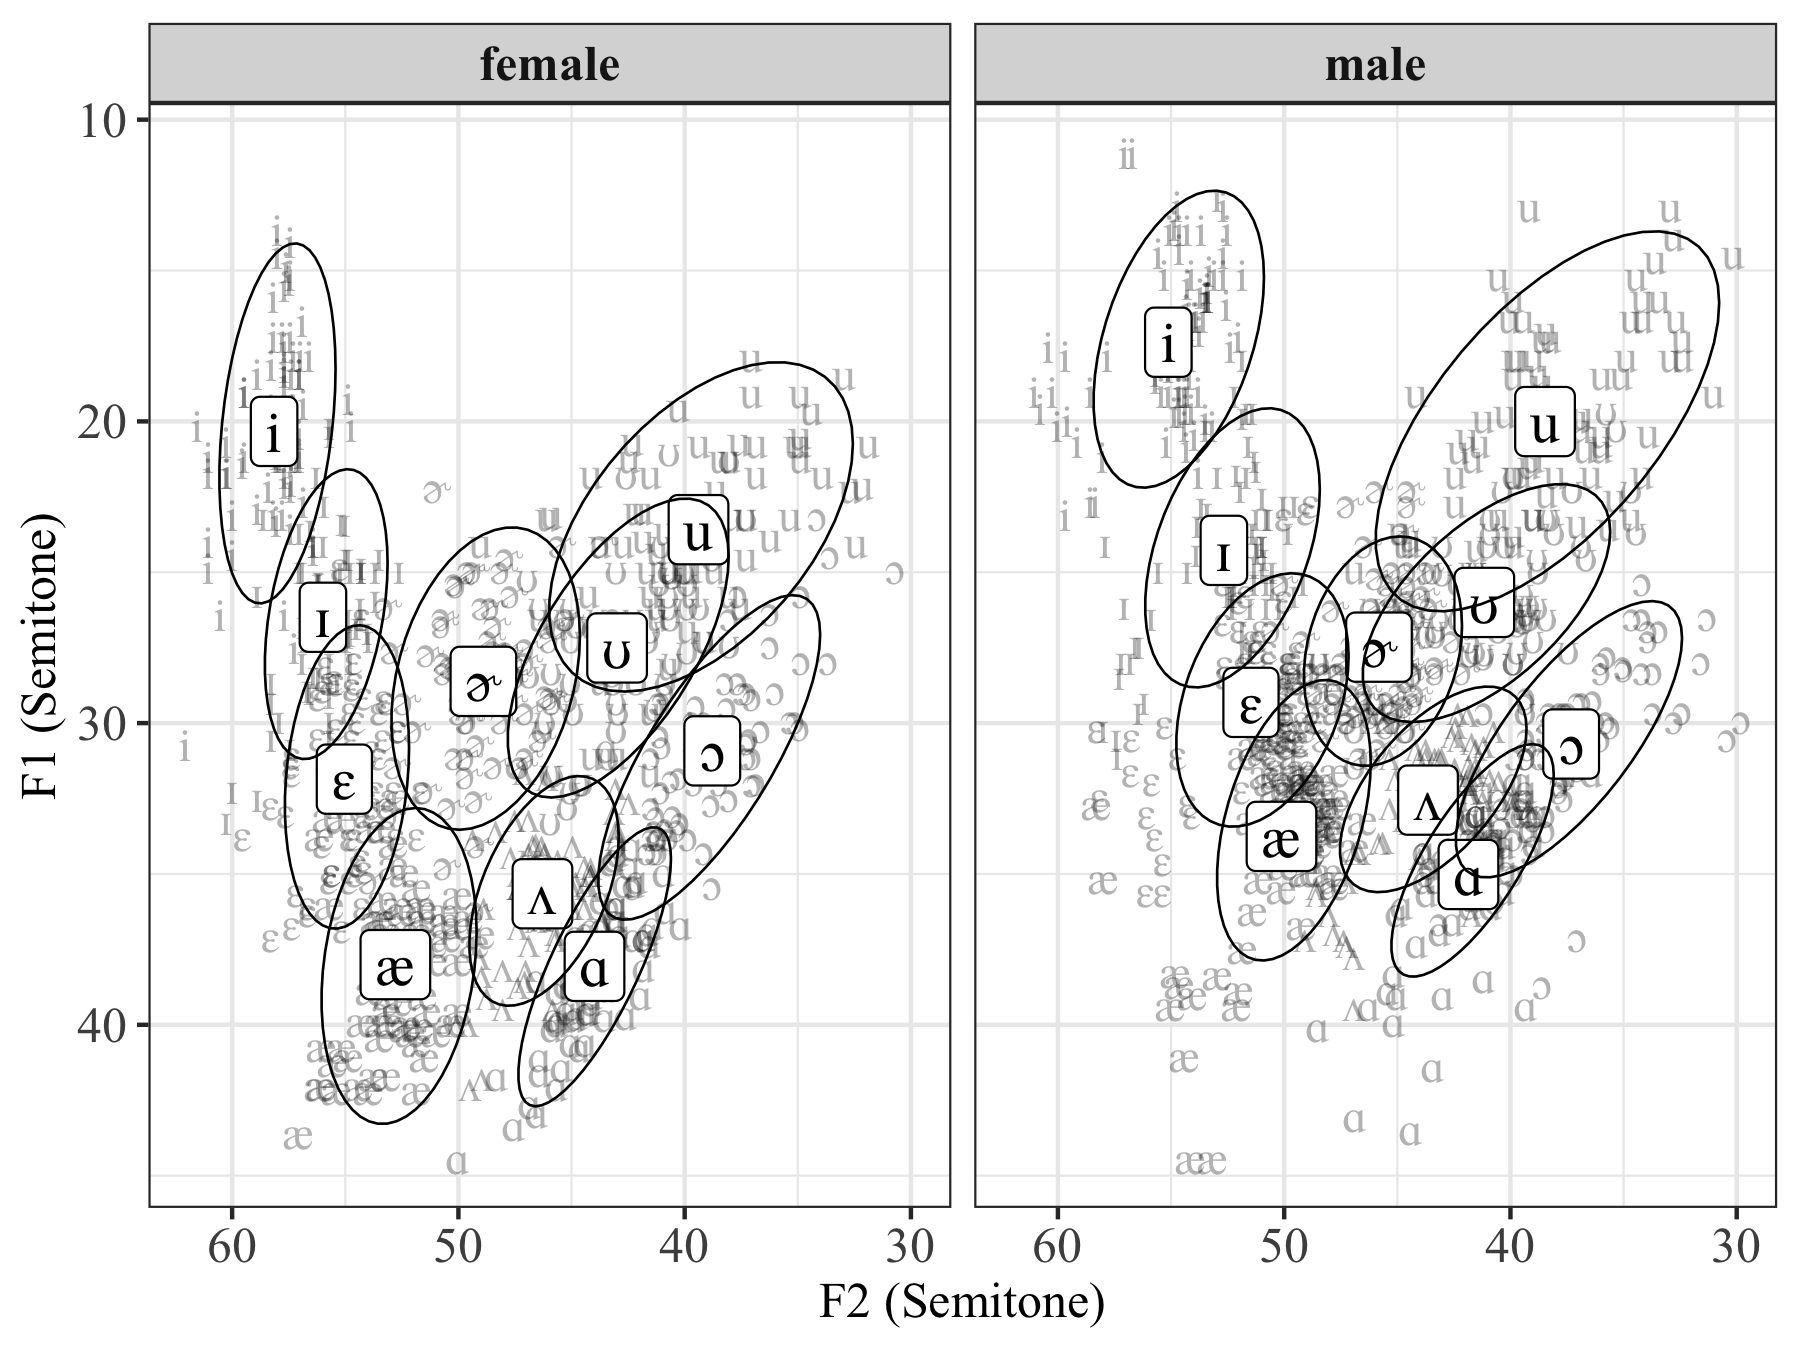
\includegraphics[width=0.75\textwidth]{figures/nativeVowel.png}
    \caption{Vowel Space of 10 American English Vowel Phonemes}
    \label{fig:nativeVowel}
  \figSpace
\end{figure}

As shown in Figure 2.1, F1-F2 spaces of some vowels encroach on the spaces of other vowels. This phenomenon makes it possible for some vowel productions to be considered allophonic variants of more than one vowel phoneme. It is, thus, possible that the encroachment of vowel space on the F1-F2 plane could potentially obfuscate the perceptual categorization of vowels. Such a claim was supported by Ladefoged (1989) who showed that the same test pronunciation /bɪt/ could be perceived as “bit” by some L1 English listeners, but as “bet” by other L1 English listeners.

The current study investigates the effect of categorizability on accentedness judgment.  If accentedness perception depends on how easily an L2 speech sound can be categorized into its target L1 sound category, then consonant changes (e.g., using [ʃ] instead of [tʃ]) might be more accented than vowel changes (e.g., using [ʌ] instead of [æ]), because consonants are more categorizable. Given the relatively higher categorizability of consonants, it is expected that listeners will more likely agree on which consonant phoneme they hear in an utterance. Disagreements might emerge when vowels are concerned. If the categorizability of speech sounds participates in accentedness judgment, then judgments on consonants produced by L2 speakers could be more consistent than judgments on vowels produced by L2 speakers.  

\section{Lexical Identification}

Another possible difference between consonant and vowels lies in their respective role in lexical identification. Previous research often claims that consonants are more important than vowels in lexical identification \citep{Nespor_2003}. Studies in lexical identification often attributes the difference between consonants and vowels to their phonological-distributional properties \citep{Nespor_2003}. They claim that vowels are more variable than consonants in continuous speech. Listeners who are accustomed to contextual variabilities of vowels would therefore choose to rely on consonants to identify words \citep{Cutler_2000}. If lexical identification participates in one’s judgment of accentedness, then perhaps consonant changes would be considered more accented, because lexical identification depends more on consonants than vowels. 

Since vowels are generally longer and louder than consonants \citep{Ladefoged_1996}, one would intuitively assume that vowels are more salient to listeners and should consequently be more reliable in lexical identification. However, results from previous empirical studies have shown just the opposite. For example, participants of \citep{Bonatti_2005} preferred identifying words in continuous speech using the transitional probability (TP) between consonants, rather than TP between vowels. TPs of speech sounds are defined as the conditional probabilities of sound B, given A. Intuitively, the TP between A and B could be interpreted as the probability for B to follow A in the same word (e.g., how probable it is for /s/ to follow /k/ in the same word). 

In \citet{Bonatti_2005}, participants first listened to nonce words of an artificial language (e.g., /mulitɛ̃/, /mylɔ̃ta/, /budikɛ̃/, /bydɔ̃ka/). The words were designed to keep TPs between consonants and TPs between vowels of a word constant (e.g., consonants /m, l, t/ and /b,d, k/ always occurring in the same order in a word, vowels /u, i, ɛ̃/ and /y, ɔ̃, a/a row in a word).

After being exposed to the nonce words, participants heard two more types of nonce words. The first type, called the CT words, changed vowel sequences, but kept consonant sequences the same as the words heard during the exposure phase (e.g., /mɔ̃latɑ̃/, /bidɛ̃ky/). The second type, called the VT words, kept vowel sequences the same as before but changed consonant sequences (e.g., /dukimɛ̃/, /ʀyɡɔ̃ma/). Participants judged the CT words to be more similar to words they heard during the exposure phase, suggesting that consonant information was more salient than vowel information to the participants. 

 In van Ooijen (1996)’s word reconstruction test, participants were asked to change a nonce word (e.g., \textit{kebra}, \textit{eltimate}) to a real word by changing either the first consonant (e.g., turn \textit{kebra} to \textit{zebra}, turn \textit{eltimate} to \textit{estimate}) or the first vowel (e.g., turn \textit{kebra} to \textit{cobra}, turn \textit{eltimate} to \textit{ultimate}). Participants overwhelmingly preferred changing the vowels, rather than changing the consonants. When specifically asked to change only the consonant or only the vowel, participants were significantly better at performing vowel changes than consonant changes. These results were replicated by \citep{Cutler_2000}, who performed experiments on Dutch and Spanish speakers, using Dutch or Spanish words as stimuli. \citet{Cutler_2000} further showed that the preference for vowel alternations was unrelated to the consonant-to-vowel ratio in a specific language. Results from these studies show that listeners, regardless of their linguistic background, tend to tolerate vowel changes more so than consonant changes.

\citet{Bonatti_2005, Van_Ooijen_1996}’s results have significant implications in foreign accent research. Thus, if consonant information is truly more important than vowels in lexical identification, then consonant change in L2 speech would be considered a more severe departure from its L1 target, which could potentially lead to a higher degree of foreign accentedness. However, if accentedness judgment does not concern lexical information, then consonant and vowel changes might not differ in their accentedness. To evaluate whether lexical identification participates in accentedness judgment, lexical information of an L2 utterance needs to be taken into consideration, in addition to phonetic and phonological information. Chapter \ref{ch:6} discusses this issue in detail.

\section{Summary}

Previous studies have suggested that both the temporal (e.g., VOTs of plosives) and spectral (e.g., formants of liquids) aspects of consonants have an effect on accentedness ratings. The findings on vow- els were mixed, with some studies showing the effects of both temporal (e.g., vowel duration) and spectral aspects (e.g., F1 and F2) of vowels \citep{McCullough_2013}, while others showing only the spectral effects \citep{Chan_2016}. Among the studies that show spectral effects, some claim that the degree of spectral deviation from native speaker norms can predict accentedness \citep{McCullough_2013, Wayland_1997}, whereas others argue that the spectral overlapping of vowel categories is the key in foreign accent perception \citep{Chan_2016, Sidaras_2009}. Despite the disagreement, previous literature show that accentedness is affected by some phonetic feature of vowels, be it spectral overlapping of vowel categories or spectral deviation from a native speaker’s norm. Among the research on foreign accent perception, the perception of L2 syllables has not been well studied. Although there is some evidence of the relative importance of segment epenthesis, questions remain as to whether segment deletion correlates with accentedness.

The current study aims to address the potential problems in previous research by obtaining stimuli that are both natural and representative of L2 speakers from various language backgrounds. Instead of acoustic manipulation, the current study opted to pick stimuli that were already identified as containing phonetic features that are common to L2 English speakers. The current study also controls for prosody in the least intrusive manner by employing a Dynamic Time Warping method. Details of stimuli selection and this Dynamic Time Warping method are discussed in Chapter \ref{ch:4}.


Many previous studies have focused on only a few types of phonetic patterns in L2 speech The current study investigates the perceptual accentedness with a larger variety of phonetic patterns. The results provide a more detailed understanding of how different types of phonetic patterns are weighted in accentedness perception. The results are discussed in Chapters \ref{ch:4} and \ref{ch:5}.

The current study hypothesizes that consonants and vowels do not contribute to accentedness to the same degree. Since consonants and vowels differ in their perceptual categorizability, it is possible that phonemic alternations of consonants and vowels are perceived differently, which could in turn affect their perceptual accentedness. Since consonants and vowels were often observed by previous literature to function differently in lexical identification, it is possible that consonant and vowel changes exhibit different degrees of foreign accentedness. Based on previous research on L2 syllable structures, the current study hypothesizes that segment epenthesis is perceptually more accented than segment deletion because segment deletion is sometimes allowed in L1 speech, while segment epenthesis rarely occurs. The current study empirically examines these hypotheses in Chapters \ref{ch:4} and \ref{ch:5}.












